\documentclass[11pt,a4paper]{report}
\usepackage{a4wide}                     % Iets meer tekst op een bladzijde
\usepackage[dutch]{babel}               % Voor nederlandstalige hyphenatie (woordsplitsing)
\usepackage[utf8x]{inputenc}
\usepackage{hyperref}
\usepackage{listings}
\usepackage{color}
\usepackage{amsmath}
\usepackage{amssymb}
\usepackage{parskip}
\usepackage{graphicx}
\usepackage{float}
\usepackage{caption}
\usepackage{enumitem}

\lstset{
  frame=tb,
  language=Perl,
  aboveskip=3mm,
  belowskip=3mm,
  showstringspaces=false,
  columns=flexible,
  basicstyle={\small\ttfamily},
  numbers=none,
  %numberstyle=\tiny\color{gray},
  %keywordstyle=\color{blue},
  %commentstyle=\color{dkgreen},
  %stringstyle=\color{mauve},
  breaklines=true,
  breakatwhitespace=true,
  tabsize=3
}
\graphicspath{afbeeldingen}
\setcounter{secnumdepth}{3} % how many sectioning levels to assign numbers to
\setcounter{tocdepth}{3}    % how many sectioning levels to show in ToC

\title{Besturingssystemen III \\ \Large{OLE Automation, Excel \& WMI scripting}}

\author{Bjorn Vandenbussche}
\date{2015-2016}

\begin{document}
\maketitle
\tableofcontents
\chapter{COM programmatie, Scripting Hosts en Engines}
\section{COM componenten en objecten}
Het is de bedoeling van de Windows labo's om te leren hoe de meeste taken, die op een of andere manier verband houden met het operating systeem, kunnen geautomatiseerd worden met behulp van eenvoudige scripts. Deze scripts steunen in eerste instantie op de mogelijkheid om externe \textbf{Common Object Model (COM)} objecten aan te spreken. 
\par Dankzij het COM model beschikt om het even welke toepassing (of operating systeem component) over een standaard manier om haar functionaliteit ter beschikking te stellen aan om het even welke andere toepassing. De toepassing die COM objecten ter beschikking stelt wordt een \textbf{COM server} genoemd, terwijl een toepassing die deze COM objecten gebruikt een \textbf{COM cliënt} noemt. Zowel COM servers als COM cliënts zijn \textit{taal-onafhankelijk}: je kan zowel een met VBScript ontwikkelde COM cliënt hebben die een met C++ ontwikkelde COM server aanspreekt, als omgekeerd. Bovendien kunnen COM servers en COM cliënt op verschillende machines uitgevoerd worden.
\par Een monolithische toepassing kan de aangeboden functionaliteit opsplitsen in diverse logische eenheden, die we \textbf{COM componenten} noemen. Een COM component is een container van één of meerdere COM klassen. Deze opsplitsing laat toe om de belasting te spreiden. De functionaliteit van elke COM component wordt hetzij door een Dynamic Link Library (.dll), hetzij door een executable programma (.exe) geïmplementeerd.
\newpage
\section{COM-klassen registratie}
Wanneer men op een toestel een COM server installeert, worden in de HKEY\_CLASSES\_ROOT  hive van het register de verschillende klassen die hij aanbiedt, geregistreerd. De registratie-procedure van een COM component is afhankelijk van de gekozen implementatie-methode:
\begin{itemize}
\item{dll} (Dynamic Link Library): gebruik regsvr32.exe met als parameter de $.dll$ bestandsnaam.
\item {exe} (executable programma): roep de executable op met parameter /regserver
\end{itemize}
\par De registratie slaat uiteenlopende informatie op in verband met de COM klassen, waarvan het grootste gedeelte gebruikt wordt om COM objecten te activeren. Van zodra een COM server geregistreerd is kan om het even welke COM cliënt gebruik maken van de aangeboden objecten.
\par Wanneer een COM cliënt een COM object van een bepaalde klasse aanmaakt, wordt nagegaan of de bijhorende .exe of .dll reeds geladen is. Indien dit nog niet is geladen, roept de COM api de noodzakelijke procedures op van de COM server om het object te creëren, afhankelijk van de gekozen implementatie-methode:
\begin{itemize}
\item{dll} : het laden van de .dll gebeurt in de context van het huidige proces. De corresponderende objecten noemt men \textit{in-process of in-proc servers}.
\item{exe} : indien de toepassing nog niet geladen is, wordt ze geladen in een nieuw proces, men noemt dit een \textit{out-of-process server}. Dit gebeurt echter in een speciale mode, de Embedded of Server mode, die geen vensters op de desktop creëert, en bijgevolg onzichtbaar is voor de gebruiker. Wanneer het object correct verwijderd wordt, wordt in dit geval ook de COM server afgesloten. Indien een fout optreedt in het script, wordt het proces meestal niet correct afgesloten!
\end{itemize}

\section{Type Libraries}

Een \textbf{COM type library} is een databank met de beschrijving van een of meerdere COM objecten. Zowel de beschikbare interfaces, attributen en methodes (en hun argumenten en terugkeerwaarde), als data types en symbolische constanten kunnen in de type library opgenomen worden. Type libraries kunnen zowel in de binaire code van de COM server zelf embedded worden (als resource), als opgenomen worden in stand-alone bestanden, met .tlb of .olb extentie. Type libraries worden uniek geïdentificeerd met een GUID.
\par Verschillende ontwikkelingsomgevingen laten toe om, op basis van de informatie vervat in de type libraries, te browsen door alle componenten en objecten die op een computersysteem geïnstalleerd zijn, en om informatie te bekomen over hun GUID, IID's, attributen en methodes. In Visual Basic en Office kun je bijvoorbeeld gebruik maken van de \textit{Object Browser}. Een alternatief is de \textit{OLE/COM Object Viewer}, die je kan oproepen met oleview.exe (geïnstalleerd op de labo-toestellen), thuis te downloaden .

\par Open Oleview - in de sectie Type Libraries staan alle beschikbare bibliotheken geordend op naam, er is geen zoekfunctie. Zoek de type-library van Excel - je vindt de naam van de bibliotheek (eventueel van meerdere versies) en ook de unieke GUID. Indien je nu dubbelklikt - in de linkerkolom - op de gevonden type library dan kan je de interfaces en de symbolische constanten doorbladeren. Zoek de groep symbolische constanten "XlVAlign" die 5 constanten bevat die we in reeks 2 zullen nodig hebben.

\section{Object hiërarchieën}

Praktisch de volledige Windows Server functionaliteit, en ook zeer veel commerciële toepassingen, volgen het COM model. Uiteraard is het de COM server die de naamgeving van zijn klassen, en de methoden en attributen die ze vervatten, bepaalt. Om met een COM model te kunnen werken (welke klassen, attributen, methodes ? ...) is het belangrijk dat je documentatie kan raadplegen. 
\par Uiteraard kan je op het internet heel veel informatie bekomen, maar de COM modellen die in deze labo's aan bod komen worden allemaal gedocumenteerd in de \textit{MSDN Library van Visual Studio 2008}. Op de labo-toestellen staat deze reeds geïnstalleerd. Deze documentatie, die off-line is, mag je ook gebruiken tijdens de oefeningentesten. Leer dus om informatie snel op te zoeken !! Er is ook een on-line versie (o.a. geïntegreerd in Visual Studio 2010), maar die is anders gestructureerd en kan je niet gebruiken op de testen. Interessante takken met informatie zullen regelmatig vermeld worden, en worden samengevat in een overzicht, dat je mag gebruiken bij de testen.
\par De meeste COM objecten bevatten methoden of attributen die andere objecten of collecties (=verzameling van objecten) creëren. De methodes en attributen van deze nieuwe objecten kunnen op hun beurt weer andere objecten creëren, ..., en zo verder. Door een COM object te initialiseren beschikt men dus over een hele structuur van verwante objecten. Het geheel van objecten noemt men een \textbf{object hiërarchie}. Een object hiërarchie start doorgaans met een object op basisniveau, en omvat objecten die meer specifieke aspecten van de toepassing of van het operating systeem omschrijven. Op elk niveau van de hiërarchie bevatten de objecten zowel attributen en methodes om de koppeling te maken met objecten lager in de hiërarchie, als attributen en methodes om de specifieke informatie op dat niveau aan te spreken.

\section{Object Interfaces}

Alle objecten hebben één of meer interfaces. Een COM interface wordt geconstrueerd als een pointer naar een tabel, de virtual function table of vtable, van pointers, die elk verwijzen naar een functie in de implementatie van een attribuut of van een methode. Voor elk attribuut van een klasse zijn er meestal twee functies in de vtable: één die de waarde ervan weergeeft (bijvoorbeeld $get\_attribuut$), en één die de waarde kan wijzigen (bijvoorbeeld $put\_attribuut$). 
\par De gezamenlijke interfaces definiëren de mogelijke communicatie tussen COM cliënt en COM object: een interface definieert een aantal attributen en methodes, hun parameters en terugkeerwaarden. Elke interface is gekenmerkt door een Global Unique Identifier (GUID), die men de \textit{Interface Identifier (IID)} noemt. COM gebruikt GUID's om conflicten te vermijden tussen interfaces met eenzelfde naam. 
\par Om de backward compatibiliteit van COM componenten te verzekeren, mogen de specificaties van interfaces niet gewijzigd worden, eens de component verspreid is. Indien men toch de parameters van een bestaande method, of aanvullende attributen en methodes wil invoeren, moet dit gebeuren door de oude interface te behouden, en de nieuwe functionaliteit te implementeren in een aanvullende interface. 
\par Veel ProgID's bevatten dan ook een versienummer. Klassen met ProgID's, die enkel in het versienummer verschillen, vertonen meestal wel hetzelfde CLSID, wat erop wijst dat ze door dezelfde COM server geïmplementeerd worden. Indien ProgID's voorkomen met versienummers, is er ook steeds een corresponderend ProgID zonder vermelding van het versienummer. In de registertak van dit ProgID staat er dan een CurVer registersleutel, die verwijst naar de meest recente ProgID. Vanuit applicaties hoef je bijgevolg zelden te refereren naar klassen met een expliciete versie specificatie.
\par Een interface heeft traditioneel een naam die start met de hoofdletter I. Elk COM object moet een IUnknown interface voorzien. In diagramma's die een COM object symboliseren, tekent men deze interface traditioneel aan de bovenzijde van het COM object. IUnknown implementeert drie methodes:
\begin{itemize} 
	\item \textit{QueryInterface} wordt gebruikt om uit te vissen of het object ook andere interfaces bezit,
\item telkens één of andere COM cliënt een referentie naar een specifiek object verkrijgt, wordt voor dit object een referentieteller verhoogd door middel van de \textit{AddRef method},
\item wanneer de referentieteller, na eventueel herhaalde oproepen van de \textit{Release method}, uiteindelijk weer de waarde nul bereikt (en er bijgevolg geen enkele COM cliënt nog langer naar refereert), verwijdert het object zichzelf uit het geheugen.

\end{itemize}

\section{OLE Automation en Binding}
\par Opdat een COM cliënt een object zou kunnen gebruiken, moet de toepassing eerst intern informatie over het object opslaan. Men noemt dit het \textit{binden van het object}. De meest efficiënte manier hiervoor wordt \textit{tijdens compilatie van de COM cliënt uitgevoerd} en daarom \textbf{early binding of vtable binding} genoemd. 
\par Early binding is zeer snel: tijdens compilatie wordt eenmalig het adres van de implementerende functie uit de vtable gehaald, en in de binaire programmacode opgeslagen. Tijdens uitvoering wordt er hierdoor nagenoeg geen verschil gemerkt tussen uitvoering van een gewone functie, en een functie die een attribuut of methode van een COM object verwezenlijkt. 
\par Early binding laat, dankzij type libraries (zie reeks 2), ook \textit{syntax checking} van de argumenten toe. Anderzijds reserveert early binding sowieso geheugen voor de structuur van het object, onafhankelijk of het object tijdens effectieve uitvoering gebruikt wordt of niet. 
\par Early binding is \textit{niet beschikbaar in geïnterpreteerde omgevingen}. Het ontwikkelen van een eenvoudige COM cliënt, die van early binding gebruik moet maken, bijvoorbeeld in C++, is niet voor iedereen triviaal ! Om een nieuw object te creëren moet het programma zelf, via de CoCreateInstance COM functie, verwijzen naar de CLSID van de COM klasse en de IID van de specifieke interface. Om te refereren naar een bestaand object kan een C++ programma gebruik maken van de CoGetObject COM functie. Het programma moet bovendien zelf de Release functie van de interface oproepen, om ervoor te zorgen dat het object zichzelf na gebruik opruimt. De geïnteresseerden in de Microsoft Agent Control COM server, waarvan het voorbeeld gebruik maakt, kunnen best de msagent.chm en msagent.chi helpbestanden downloaden om het overeenkomstige object model te bestuderen. Dit wordt niet verder behandeld in deze labo's.

\par We beperken ons tot de \textbf{late binding}, waarbij de binding tussen de COM cliënt en het object slechts wordt verwezenlijkt tijdens uitvoering van de COM cliënt. De binding gebeurt \textit{op basis van de ProgID}, andere details van het object moeten hierdoor niet a priori gekend zijn. 
\par De COM cliënt moet zich niets aantrekken van het bestaan van (diverse) interfaces. Hierdoor is het programmeren van een script versie van een COM cliënt een stuk eenvoudiger.
Maar... \textit{late binding is enkel mogelijk indien voor het COM object ook de optionele interface IDispatch aanwezig is}. Deze moet vier methodes implementeren:
\begin{itemize}
\item \textit{GetTypeInfo} en \textit{GetTypeInfoCount} kunnen gebruikt worden om de methodes en attributen van een object af te scannen,
\item de \textit{GetIDsOfNames} methode wordt gebruikt om op basis van de naam van een attribuut of methode een numerieke identificatie, de dispatch ID of DispID, van de implementerende functie te bekomen, 
\item de \textit{Invoke} methode voert een implementerende functie uit op basis van de dispatch ID.
\end{itemize}
\par Objecten met de IDispatch interface worden \textbf{automation objecten} genoemd en laten late binding toe. Late binding is echter traag: telkens bij uitvoering een attribuut of methode van het object aangesproken wordt, moet eerst de GetIDsOfNames en vervolgens de Invoke functie van de IDispatch interface uitgevoerd worden. Indien methodes van objecten foutief aangesproken worden, kan dit bovendien enkel bij uitvoering gedetecteerd worden.
\par Geïnterpreteerde talen ondersteunen enkel late binding, en bijgevolg enkel COM objecten met een automation interface. De meeste COM objecten ondersteunen een duale interface en stellen hun functies zowel onrechtstreeks via de IDispatch interface als rechtstreeks via de vtable ter beschikking. Hierdoor kunnen deze zowel op een snelle manier aangesproken worden door toepassingen die early binding ondersteunen, als door geïnterpreteerde omgevingen.

\section{COM technologieën met een automation interface}

Componenten met een automation interface kunnen vanuit geïnterpreteerde omgevingen gemanipuleerd worden. Ten opzichte van gecompileerde programma's vertonen scripts belangrijke \textbf{nadelen}:
\begin{itemize}
\item de uitvoering van scripts is veel \textit{trager}.
\item scripts zijn \textit{minder goed beschermd} tegen piraterij. Ze kunnen (meestal) gekopieerd en gewijzigd worden door iedereen die de scripts moeten kunnen uitvoeren. Recente aanvullingen zoals script encoding laten toe om de intellectuele eigendom van de programmeur beter te beschermen.
\item \textit{syntax fouten} worden pas in een veel later stadium ontdekt.
\end{itemize}
Toch zijn er ook heel wat \textbf{voordelen}:
\begin{itemize}
\item scriptomgevingen vormen voor veel mensen (zelfs voor professionele programmeurs) een \textit{minder hoge moeilijkheidsdrempel}, waardoor ook voor hen het volledige beheer van COM objecten met automation interface uitvoerbaar wordt
\item het ontwikkelen van scripts vergt \textit{geen complexe ontwikkelingsomgeving}, die reeds op zich dikwijls moeilijk te configureren en aan te leren is
\item scripts zijn uitermate geschikt voor een snelle, geautomatiseerde oplossing van \textit{kleine problemen} en taken
\item dankzij markup talen zoals HTML en XML is men \textit{niet aangewezen op één enkele programmeertaal}, maar kunnen scripts in verschillende talen gecombineerd worden tot een oplossing in tekst formaat, die bovendien het voordeel biedt om door om het even welke web browser gedownload te kunnen worden
\end{itemize}
\par De meeste objectmodellen van Microsoft software (zowel van operating systeem componenten, als van toepassingen), voorzien in een \textbf{automation interface}. Hieronder wordt een sumier overzicht gegeven van de huidige technologieën met een automation interface. Een aantal onder hen komen in de volgende reeksen meer uitgebreid aan bod:
\begin{itemize}
\item De Windows Management Instrumentation (WMI) technologie is een implementatie van een ruimere standaard, \textbf{Web Based Enterprise Management (WBEM)} genoemd. WMI kan nagenoeg alle resources van een Windows Server computer beheren: het operating systeem zelf, hardware en device drivers, de BIOS, het register, security informatie en het bestandssysteem. Met een paar lijnen WMI code kun je bijvoorbeeld een overzicht bekomen van alle processen, en hun Process Identifier. We bespreken het object model van WMI in deze labo's (reeksen 3 en 4). Dit model kan zelfs programmatisch uitgebreid worden, maar dit aspect zal niet aan bod komen in de labo's.
\item De \textbf{ActiveX Data Objects (ADO)} specificatie voorziet in een verzameling objecten die generieke toegang mogelijk maken tot een hele reeks locale en remote databanken (ondermeer e-mail repositories en relationele databank omgevingen zoals Access, Oracle en SQL Server)
\item Het \textbf{Collaboration Data Objects (CDO)} object model laat scripts toe te interageren met mail servers, zoals Exchange. Hierdoor kan men bijvoorbeeld programmatisch mailboxen aanmaken en e-mail versturen. We zullen in de volgende reeks een eerste voorbeeld met dit COM - model uitwerken.
\item Alle componenten van recente Office suites (Office 97, Office 20xx) kunnen volledig door scripts gestuurd worden. In reeks 2 zullen we ter illustratie hiervan een oefening maken gebaseerd op het Excel  object model.
\item Internet Explorer is volledig beheersbaar vanuit scripts, en laat ondermeer toe om actieve pagina's te ontwikkelen waarin cliënt-side scripts uitgevoerd worden. Cliënt-side scripts genereren de output dynamisch en interageren met de gebruiker.
\item De \textbf{Active Directory Services Interface (ADSI)} biedt COM toegang, zowel tot de volledige Active Directory van een Windows Server domein, als tot de gebruikersdatabank van een NT domein of de lokale gebruikersdatabanken van individuele NT en Windows toestellen. ADSI wordt in deze labo's uitvoerig behandeld in reeksen 6-8.
\end{itemize}

\section{ActiveX Scripting}

Om toe te laten deze verschillende technologieën zowel vanuit verschillende toepassingen als met behulp van diverse scripttalen aan te kunnen spreken, voorziet de ActiveX Scripting architectuur in een \textit{stricte scheiding tussen script hosts en script engines}. De script engines ondersteunen de feitelijke programmeertaal, terwijl de script hosts de interface vormen tussen deze taal en een willekeurige toepassing die ervan gebruik wil maken. De script host zorgt ervoor dat een script instructie per instructie gelezen en uitgevoerd wordt. De ActiveX Scripting architectuur maakt het mogelijk dat om het even welke script host kan gecombineerd worden met om het even welke script engine.
\par Voorbeelden van populaire script engines zijn VBScript, JScript, PerlScript, Python en Tcl. In deze labo's wordt geopteerd voor PerlScript. PerlScript, geïmplementeerd door perlSE.dll, is een goed voorbeeld van een ActiveX scripting engine, die kan gebruikt worden in combinatie met om het even welke andere ActiveX scripting host. Omdat de meeste voorbeelden in de MSDN Library geschreven zijn in VBScript, zal ook de syntax van VBScript kort besproken worden.

Om het even welke script host kan optreden als COM cliënt. Voorbeelden van belangrijke scripting hosts zijn:
\begin{itemize}
\item de Windows Scripting Host (WSH)
\item Perl kan als host fungeren, maar dan wel enkel met Perlscript als engine,
\item de Active Server Pages (ASP) technologie, die hetzij Internet Information Server (IIS), hetzij een Personal Web Server (PWS) vereist, 
\item de Internet Explorer web browser,
\item Microsoft Office toepassingen,
\item zelf ontwikkelde Windows Script Components.
\end{itemize}
In de labo's gebruiken we hoofdzakelijk de mogelijkheid om COM-objecten te gebruiken vanuit perl. Hierbij is perl.exe eigenlijk terzelfdertijd (monolitisch) de host en de engine. 
Er wordt ook een inleiding gegeven op PowerShell.
\section{Voorbeelden}
\begin{enumerate}
	\item Bekijk het register met de commando's \textit{regedit} of \textit{regedt32} (vanaf Windows Server 2003 roepen deze hetzelfde programma op). In de HKEY\_CLASSES\_ROOT hive vind je een alfabetisch overzicht van alle klassen. Voor elke klasse wordt een afzonderlijke subtak in het register gecreëerd, met als identificatie de Programmatic Identifier, afgekort ProgID. De ProgID vervult een belangrijke rol als brug naar de buitenwereld: een COM cliënt vraagt een COM object door het opgeven van het ProgID.
	\par Zoek in het register \textit{de klassen die Excel aanbieden}, waaronder de klasse \textit{Excel.Sheet} (in meer dan 1 versie). Zoek ook ook de klassen \textit{CDO.Message} en \textit{Scripting.FileSystemObject}. 
	\par De registertak van elke klasse bevat een subtak CLSID, die een element bevat met als waarde de GUID, een 16-byte hexadecimale string die de klasse uniek identificeert. Zoek de GUID op van de klassen \textit{Excel.Sheet} , \textit{CDO.Message} en \textit{Scripting.FileSystemObject}.
	\par De CLSID tak van de HKEY\_CLASSES\_ROOT hive bevat een subtak voor elke GUID.
	Bij een 64bit systeem, is de situatie wat complexer. Er is namelijk een tweede CLSID tak, onder de tak WOW6432Node, daar vind je een subtak voor elke GUID die als 32bit werd geïnstalleerd.
	
	In die GUID-subtak staat verschillende informatie. De subtak ProgID bevat het juiste ProgID van de klasse. Bepaalde informatie is afhankelijk van de gekozen implementatie-methode:
	\begin{itemize}
	\item dll : InprocServer32 verwijst naar de bijhorende .dll, zoals bij de klassen CDO.Message en Scripting.FileSystemObject
	\item exe : LocalServer32 verwijst naar de bijhorende .exe, zoals bij de klasse Excel.Sheet
	\end{itemize}	
	Zoek deze informatie op in het register.
	\\
\begin{lstlisting}
GUID van Scripting.FileSystemObject is 0D43FE01-F093-11CF-8940-00A0C9054228, met ProgID "Scripting.FileSystemObject" 
en is geimplementeerd als dynamic link library (srcrun.dll)

GUID van CDO.Message is CD000001-8B95-11D1-82DB-00C04FB1625D, met ProgID "CDO.Message" 
en is geimplementeerd als dynamic link library (cdosys.dll)

GUID van Excel.Sheet.5  is 00020810-0000-0000-C000-000000000046, met ProgID "Excel.Sheet.5"
GUID van Excel.Sheet.8  is 00020820-0000-0000-C000-000000000046, met ProgID "Excel.Sheet.8"
GUID van Excel.Sheet.12 is 00020830-0000-0000-C000-000000000046, met ProgID "Excel.Sheet.12"
GUID van Excel.Sheet    is 00020830-0000-0000-C000-000000000046  en verwijst dus naar de laatste versie
Enkel de recentste versie is geimplementeerd als executable (excel.exe).
\end{lstlisting}
\newpage
	\item In het register vind je voor bepaalde COM-klassen ook de bijhorende Type Library. Zoek of je in de CLSID subtab een verwijzing vindt naar TypeLib. Soms word je doorverwezen naar een andere COM-klasse voor deze informatie. Soms ontbreekt deze subtak, maar is er wel een Type Lybrary bij die COM-klasse.
	\par Zoek de GUID op van de Type Libraries die horen bij de COM-klassen \textit{Excel.Sheet.5} en \textit{CDO.Message}. Je vindt hier, jammer genoeg, niet de naam van de bibliotheek...
	\\
\begin{lstlisting}
"Excel.Sheet.5" met CLSID 00020810-0000-0000-C000-000000000046, 
verwijst (AutoConvertTo) door naar het COM-object met CLSID 00020820-0000-0000-C000-000000000046 ("Excel.Sheet.8").

Daar vind je de Type Library met GUID 00020813-0000-0000-C000-000000000046. 
De naam zoek je op in "Oleview" en is "Microsoft Excel 12.0 Object Library".

"Scripting.FileSystemObject" met CLSID 0D43FE01-F093-11CF-8940-00A0C9054228 bevat een "Type-Library" met GUID 420B2830-E718-11CF-893D-00A0C9054228
Deze vind je waarschijnlijk niet terug in "Oleview" - indien wel graag even melden.

"CDO.Message" met CLSID CD000001-8B95-11D1-82DB-00C204FB1625D bevat geen tak met "Type Library" en verwijst niet door.
Nochtans is er een bijhorende bibliotheek die je terugvindt in  "Oleview". 
Deze is namelijk "Microsoft CDO for Windows 2000 Library"  met GUID CD000000-8B95-11D1-82DB-00C04FB1625D.

\end{lstlisting}
\end{enumerate}
\chapter{COM programmatie in de praktijk}
We bespreken in deze reeks de basisprincipes van COM programmatie met scripts. //
Een Windows script is een tekstfile, geschreven in een scripttaal (Script Engine). Een Windows script wordt niet gecompileerd in .exe vorm, maar is volledig aangewezen op een Scripting Host om zijn code at runtime uit te voeren.
\par Elke scripting host biedt een omgeving aan die zorgt voor de correcte uitvoering van elk script, geschreven in een taal waarvoor de ActiveX script engine geïnstalleerd is. De meeste scripting hosts zijn toepassingen (zoals Internet Explorer zie hoofdstuk 5).
\par De volgende Scripting Hosts, die vanuit een Command Prompt console worden opgestart, zijn uitermate geschikt voor operating systeem verwante taken:
\begin{itemize}
\item WSH: Window Scripting Host  , gecombineerd met VBScript, JavaScript of Perlscript als scripting Engine.
\item Perl: enkel in combinatie met engine PerlScript
\end{itemize}
In deze labo's beperken we ons tot het gebruik van Perl als scripting Host.

\section{Scripting engines : VBScript / PerlScript}
De meeste voorbeelden in de MSDN Library zijn geschreven in VBScript. Deze voorbeelden kan je \textit{niet} uittesten met perl als host. We geven toch een korte vergelijking tussen VBScript en PerlScript, zodat je de voorbeelden kan omzetten naar Perlscript.
\par Hieronder een kort overzicht met belangrijke verschillen:\\
\begin{tabular}{|l|l|l|}
	\hline  & \textbf{VBScript} & \textbf{PerlScript} \\ 
	\hline  Case-sensitive & nee & ja \\ 
	\hline  Commentaar & ' comment & \# comment \\ 
	\hline  Afsluiten statement & nieuwe regel & ; toevoegen \\ 
	\hline  Declaratie verplicht maken & Option explicit & use strict; \\ 
	\hline  Variabele declareren & Dim varnaam & my \$varnaam \\ 
	\hline  COM-object toekennen & Set varnaam = & \$varnaam= \\ 
	\hline  Attribuut opvragen van object & varnaam.attribuutnaam & \$varnaam$\rightarrow$\{attribuutnaam\} \\ 
	\hline  Methode uitvoeren van object & \parbox[t]{5cm}{\$varnaam.\\methodenaam(argumenten)} &
	\parbox[t]{5cm}{\$varnaam$\rightarrow$\\methodenaam(argumenten)} \\
	\hline 
\end{tabular} 
\par \textbf{Merk op:}
\begin{itemize} 
	\item In een scripttaal heeft een variabele geen specifiek type en moet dus niet gedeclareerd worden. Het grote nadeel hiervan is dat domme typfouten in een variabelenaam niet gemakkelijk opgespoord worden. Je kan declaratie toch verplicht maken.
	\item In VBScript moet je de Set instructie gebruiken om een COM-object toe te kennen aan een variabele, in PerlScript is dit een gewone toekenning.
	\item In PerlScript wordt een referentie naar het object opgeslaan in de variabele, waardoor de attributen en methodes met -> worden opgevraagd en dus niet met de punt-notatie.
\end{itemize}
Uiteraard heeft elke taal zijn eigen functies, statements en bijzonderheden, waarvoor je best de documentatie raadpleegt. 

\section{Modules gebruiken in PerlScript}
Perl(Script) stelt een enorme hoeveelheid extra functionaliteit ter beschikking met behulp van modules. Je kan een overzicht raadplegen en ook PerlScript modules downloaden op CPAN, of met de ppm opdracht.
\begin{enumerate}
	\item Informatie over de ingeladen modules vind je in de hash \%INC, zoals in onderstaand voorbeeld wordt geïllustreerd. Je krijgt hierdoor toegang tot de geëxporteerde functies uit de module.
	In de inleiding werd de module strict reeds vermeld. Als je deze module inlaadt worden declaraties verplicht gemaakt. Welke submodules worden hierdoor ingeladen? (Je moet nu wel alle variabelen ook declareren.)
\begin{lstlisting}
while (($key,$value)=each %INC) {
	print "\$INC{$key} = $value\n";
} 
\end{lstlisting}
\end{enumerate}

\par Met Perl als host kan je niet automatisch COM-objecten initialiseren. In de Perl-documentatie, de sectie Using OLE with Perl, staat beschreven dat je hiervoor de OLE-module inlaadt met:
\par use Win32::OLE qw(in  with);
\par Onderzoek welke sub-modules nu worden ingeladen.
Deze module bevat een aantal interessante/noodzakelijke functies en methodes om COM objecten te initialiseren en te gebruiken vanuit Perlscript. De beschrijving van alle beschikbare functies en methodes zoek je op in dezelfde Perl-documentatie in de sectie Modules / Win32 / OLE (in de linkerkolom bijna helemaal naar beneden scrollen).
Een korte bespreking van de interessantste functies:
\begin{enumerate}[resume]
\item Initialiseren van COM-objecten met het ProgID
De VBScript-engine beschikt over de functie \textit{Createobject(ProgID)} waarmee je een COM-object kan initialiseren.
\par set cdo = CreateObject("CDO.Message")
\par In PerlScript gebruik je hiervoor de functie \textit{new(ProgID)} van de Win32::OLE module.
\begin{lstlisting}
use Win32::OLE;            #inladen module zonder "in" en "with" functie volstaat
$cdo = Win32::OLE->new("CDO.Message"); #functie new correct gebruiken
print ref $cdo;            #controleren of het gelukt is    
\end{lstlisting}
\end{enumerate}
\begin{enumerate}[resume]
	\item Met \textit{QueryObjectType} bekom je extra informatie over het type van een COM object. Vergelijk dit met de informatie die je met ref kon opvragen.
	\begin{lstlisting}
use Win32::OLE;

$cdo = Win32::OLE->new("CDO.Message");
printf "CDO.Message: %s  -- %s\n", ref($cdo),join(" / ", Win32::OLE->QueryObjectType($cdo));

$fso = Win32::OLE->new("Scripting.FileSystemObject");
printf "Scripting.FileSystemObject:  %s  -- %s\n", ref($fso),join(" /", Win32::OLE->QueryObjectType($fso));

$excel = Win32::OLE->new("Excel.Sheet");
printf "Excel.Sheet:  %s  -- %s\n", ref($excel),join(" / ", Win32::OLE->QueryObjectType($excel));
	\end{lstlisting}
	\item Met \textit{EnumAllObjects} kan je een lijst maken van alle OLE-objecten die geladen zijn. Dit kan handig zijn bij debuggen.
\begin{lstlisting}
use Win32::OLE qw(in);

$excel = Win32::OLE->new("Excel.Sheet");
$fso = Win32::OLE->new("Scripting.FileSystemObject");
$cdo = Win32::OLE->new("CDO.Message");

$Count = Win32::OLE->EnumAllObjects(
	sub {
		my $Object = shift;
		printf "\n%-30s : %s",ref($Object),join(" / ", Win32::OLE->QueryObjectType($Object));
	}
);
print "\n$Count OLE-objecten geladen\n";
\end{lstlisting}
\newpage
	\item Indien een fout optreedt zal het perlScript niet stoppen. Je kan echter met behulp van \textit{LastError()} de foutmelding opvragen. Probeer dit zelf uit door een fout ProgId in te geven.
\begin{lstlisting}
use Win32::OLE;
$foutobject = Win32::OLE->new("CDO.Mesage");
print "\nlast error= ",Win32::OLE->LastError();
\end{lstlisting}
	\item Een interessante mogelijkheid is de class variabele \textit{Warn instellen op 3}. Hierdoor zal bij elke fout het script wel stoppen en ook de foutmelding uitschrijven, zonder dat je dit zelf expliciet vraagt. In de Perl documentatie vind je informatie over deze variabele en de betekenis van de waarden bij Modules / WIN32 / OLE.
\begin{lstlisting}
use Win32::OLE;
$Win32::OLE::Warn = 3;
# of
# Win32::OLE->Option(Warn => 3);

$foutobject = Win32::OLE->new("CDO.Mesage");
\end{lstlisting}
\end{enumerate}

\section{De Type Library gebruiken}
Geïnterpreteerde omgevingen (zoals scripts) kunnen een beroep doen op \textit{type libraries}, maar enkel om gebruik te maken van de erin gedefiniëerde symbolische constanten. In de documentatie worden constanten regelmatig gebruikt, maar het is niet altijd duidelijk wat hun waarde is. In plaats van de waarden op te zoeken in de documentatie of in de bijhorende Type Library (met Oleview) is het handiger om de bibliotheek zelf in te laden.
\par Gebruik hiervoor de module Win32::OLE::Const Naam\_bibliotheek. In de Perl documentatie vind je uitgebreide informatie over de mogelijkheden van deze module.
\par Het argument Naam-bibliotheek wordt \textit{geïnterpreteerd als reguliere expressie}. Enkel indien een unieke typelibrary aan de naamgeving voldoet zal ze ook worden ingeladen. Om het opzoeken van de bibliotheek in het register te versnellen wordt deze reguliere expressie best vooraan \textit{impliciet uitgebreid met }\^{}. Voeg daarom \textit{ook een .*} toe indien de naam van de typelibrary niet begint met het opgegeven argument. Er treedt geen fout op indien er geen enkele bibliotheek aan de reguliere expressie voldoet !!

\begin{enumerate}[resume]
	\item In de vorige reeks heb je, in Oleview, de type libraries gevonden die horen bij de COM-klassen \textit{Excel.Sheet} en \textit{CDO.Message}. Laad nu beide libraries in, en schrijf een willekeurig gekozen constante uit (zoek de naam van een constante op met Oleview). Experimenteer met de reguliere expressie en kijk wat er gebeurt indien de bibliotheeknaam niet uniek is, of indien je een foute naam opgeeft.
	De typelibrary die hoort bij \textit{"Scripting.FileSystemObject"} kunnen we niet inladen met deze methode.
\begin{lstlisting}
use Win32::OLE::Const "^Microsoft CDO for Windows 2000 Library";
#use Win32::OLE::Const ".*CDO"; #volstaat om de bibliotheek te vinden
print "\ncdoSendUsingPort : ",cdoSendUsingPort; #toont de waarde

use Win32::OLE::Const "^Microsoft Excel";      
#use Win32::OLE::Const ".*Excel"; #volstaat om de bibliotheek te vinden
print "\nxlHorizontaal    : ",xlHorizontal;
print "\nniet bestaand    : ",xlHorizontaal;   #geeft de naam zelf terug
\end{lstlisting}
	\item In de module Win32::OLE::Const beschik je over de interessante methode \textit{Load} waarmee alle constanten van een typelibrary in (een referentie naar) een hash worden inladen. Toon alle constanten van een bibliotheek, waarvan je de naam als argument meegeeft met je script.
	Nu kan je snel achterhalen welke constanten in die bibliotheek zitten.
\begin{lstlisting}
#Geef als argument bijvoorbeeld "Microsoft CDO for Windows 2000 Library"
use Win32::OLE::Const;

$bibnaam=$ARGV[0];

$wd = Win32::OLE::Const->Load($bibnaam);
while ( ( $key, $value ) = each %{$wd} ) {
	print "$key :$value\n";
}
\end{lstlisting}
	\item De \textit{Load} methode kan ook een OLE object als argument hebben. In Perl(Script) beschik je dus heel eenvoudig over alle constanten van een typelibrary die hoort bij een specifiek COM-object, ook al ken je de juiste naam niet.
	Gebruik deze methode om een overzicht te tonen van alle constanten van de drie COM-object die we tot nu toe gezien hebben. Orden nu ook dit overzicht op de constantennaam.
\begin{lstlisting}
use Win32::OLE::Const;

@ARGV=("Excel.Sheet","Scripting.FileSystemObject","CDO.Message"); #lukt altijd.

for $comObjectNaam (@ARGV) {
	print  "\n**********",$comObjectNaam,"***********\n";
	$object = Win32::OLE->new($comObjectNaam);
	%wd = %{Win32::OLE::Const->Load($object)}; #direct in een hash stoppen
	
	foreach (sort {$a cmp $b} keys %wd) {
		printf ("%30s : %s\n",$_,$wd{$_});
	}  
}
\end{lstlisting}
\end{enumerate}
\section{FileSystemObject model}
Om bestanden, folders, drives,... te bewerken/beheren in een script gebruik je het run-time object \textbf{FileSystemObject (FSO)}.
Een overzicht hiervan vind je in de MSDN Library in Web Development / Scripting / Windows Script Technologies / Script Runtime / FileSystemObject Object.
\par Het FSO object model is een hiërarchie met objecten en collecties (die allen non-exposed zijn). Zoek de methode waarmee je een Folder, File, Drive kan ophalen. Een aantal eigenschappen van een bestand, map of drive kan je direct ophalen met een methode van het FSO object. Je kan die eigenschappen ook terugvinden in het object dat gekoppeld kan worden aan het bestand, folder of drive. Dat object heeft nog meer eigenschappen en methodes ter beschikking.
\begin{enumerate}[resume]
	\item Maak een script waarbij je een bestandsnaam opgeeft. Controleer of dit bestand gevonden wordt (in de huidige directory), en geef de volledige padnaam (kan op twee manieren) en het type van het bestand.
\begin{lstlisting}
use Win32::OLE::Const;
@ARGV=("punten.xls");
$fso = Win32::OLE->new("Scripting.FileSystemObject");
$naam=$ARGV[0];

if ($fso->FileExists($naam))
{
	$absoluutPad = $fso->GetAbsolutePathName($naam); 
	$file = $fso->getFile($naam); #absoluut of relatief
	print $absoluutPad, " bestaat en heeft type " , $file->{Type};
}
#absoluut pad kan je ook aan het File-object vragen:    
$absoluutPad = $file->{path};
\end{lstlisting}
\end{enumerate}
\section{Collections}
Een COM-hiërarchie bevat dikwijls \textbf{Collection objects}. Dit is een verzameling van objecten die individueel kunnen aangesproken worden vanuit de collectie. Meestal is de naam van een collectie object een \textit{meervoud} (bijvoorbeeld Files). Gebruik voor de variabelen die refereren naar collecties ook altijd een naam in het meervoud, om duidelijk te maken dat deze objecten diverse data elementen bevatten. 
\par De meeste collecties hebben een Count attribuut, dat weergeeft hoeveel objecten de collectie bevat. Individuele elementen van een collectie worden meestal aangesproken met behulp van de \textit{Item(index)} methode. Doorgaans is deze methode de default methode van het object, waardoor men de ->Item notatie kan weglaten, en men de indruk krijgt dat index een attribuut zou zijn. Hierdoor wordt de syntax om individuele elementen van collections aan te spreken identiek aan die om hashelementen aan te spreken.
\par De \textit{indexering} van collections moet niet altijd numeriek. Soms kan je voor dezelfde collectie, zowel numeriek als met een string indexeren. De methode van indexering wordt bepaald door de klasse van het object. Om onafhankelijk te zijn van de specifieke indexering, worden \textit{collections dikwijls afgelopen met behulp van de foreach ... (in ...)} instructie in PerlScript. Daarbij gebruik je de functie in, die door de module Win32::OLE wordt geïmplementeerd, om collections om te vormen in arrays van individuele objecten. Vergeet niet om deze functie expliciet te vermelden bij het inladen van de module.
\newpage
\begin{enumerate}[resume]
	\item Geef een lijst van alle Excel-bestanden in de werkdirectory.
\begin{lstlisting}
use Win32::OLE qw (in);
$fso = Win32::OLE->new("Scripting.FileSystemObject");
$folder = $fso->getFolder(".");
print $folder->{path};
for $file (in $folder->Files)
{
	printf "\n%s",$file->{name} if ($file->{Type} =~/Excel/);
}
\end{lstlisting}
\end{enumerate}
\section{Collaboration Data Objects (CDO) : mail versturen}
In deze paragraaf versturen we de mail door enkel gebruik te maken van COM-objecten. We gebruiken nog steeds perl als "host", en perlScript als "scripttaal", maar ook met een andere host of engine blijft deze oplossing correct werken. We beperken ons tot het versturen van een eenvoudige tekstboodschap naar één mail-adres, met behulp van het SMTP-protocol.
De hoofdbedoeling van deze oefening is dat je leert werken met COM-objecten, leert opzoeken in de documentatie en de mogelijkheden van de module Win32::OLE begrijpt.
\par Alle noodzakelijke informatie over de COM-objecten die we hiervoor nodig hebben, vind je in de MSDN Library terug in de tak WIN32 and COM Development / Messaging and Collaboration / Collaboration Data Objects (CDO) / CDO for Windows 2000.
De subtak About CDO for Windows 2000 / CDO for Windows 2000 Object Model toont de volledige hiërarchie.
\par De verdere beschrijving van alle klassen vind je terug in de subtak Reference / COM Classes. Voor onze eenvoudige mail gebruik je twee COM-klassen:
\begin{itemize}
	\item Message (progID=CDO.Message)
	\item Configuration (progID=CDO.Configuration)
\end{itemize}
\par Voor de "Message" klasse beperken we ons tot de interface IMessage. De beschikbare attributen/methodes kan je ook direct terugvinden in de tak Reference / Interfaces.
\begin{enumerate}[resume]
	\item Een eerste stap is het initialiseren van een mail-object met een Message Object - zie hiervoor. Vul gegevens in voor de afzender, de bestemmeling, het onderwerp en de inhoud. Zoek de juiste attribuutnamen op in de interface IMessage. In PerlScript bevat de variabele een referentie naar het Message Object, en moet je ->{attributeName} gebruiken.
\begin{lstlisting}
use Win32::OLE;
$mail = Win32::OLE->new("CDO.Message");
$mail->{TextBody} = 'Hallo Bjorn!';
$mail->{Subject}  = 'COM testje' ;
$mail->{From}     = 'bjorn.vandenbussche@ugent.be';
$mail->{To}       = 'bjorn.vandenbussche@ugent.be';  
\end{lstlisting}
\end{enumerate}
De methode \textit{Send()} uit de interface IMessage is verantwoordelijk voor het verzenden van de mail. Als je dit uitprobeert, dan zal de mail waarschijnlijk niet toekomen: je hebt immers niet opgegeven hoe dit moet gebeuren. (Indien Outlook Express correct geconfigureerd is via smtp, kan dit wel werken.) Toon de foutmelding voor extra informatie.
\par De Configuration-klasse is verantwoordelijk voor de instellingen. Voor deze klasse bestaat enkel de interface IConfiguration, met als enige attribuut de Fields collectie, die de "configuration settings" instelt. We bespreken eerst algemeen wat collecties zijn.
\begin{enumerate}[resume]
	\item Je kan het Configuration object initialiseren als onafhankelijk object, met zijn eigen ProgId, maar je kan dit object ook ophalen met het Configuration - attribuut van een "Message" object.
	\par Initialiseer het Configuration object en bepaal het objecttype van de objecten uit de Fields collectie. Bepaal ook het aantal objecten in deze collectie.
\begin{lstlisting}
use Win32::OLE qw(in); #vermeld expliciet de in-functie

$conf = Win32::OLE->new("CDO.Configuration");
print $conf->{Fields}->{Count}," objecten\n";

$object = $conf->{Fields}->Item(0);
print "\n",join(" / ",Win32::OLE->QueryObjectType($object));

OF

use Win32::OLE qw(in);
$mail = Win32::OLE->new("CDO.Message");
print $mail->{Configuration}->{Fields}->{Count}," objecten\n";

#Alle objecten overlopen uit de Fields-collectie
foreach (in $mail->{Configuration}->{Fields}){
	print "\n",join(" / ",Win32::OLE->QueryObjectType($_));
}
\end{lstlisting}
	\item Elk element uit de \textit{Fields collectie} is zelf een \textit{Field object}. Een Field object is eigenlijk een basisobject, dat ook in andere COM-modellen terugkomt. In de tak WIN32 and COM Development / Messaging and Collaboration / CDO 1.2.1 / CDO Library / CDO Reference vind je een uitgebreide beschrijving van o.a. dit Field object en bijhorende attributen en methoden. De belangrijkste attributen van dit Field object zijn: name, value. Geef een overzicht van de velden die standaard ingesteld zijn voor een configuration object. Bevat dit de waarden (values) die je had verwacht?
\begin{lstlisting}
use Win32::OLE qw(in);
$conf = Win32::OLE->new("CDO.Configuration");

foreach (in $conf->{Fields}){
	printf "%s = %s\n",$_->{Name},$_->{Value};
}
\end{lstlisting}
\end{enumerate}
\newpage
Waarschijnlijk bevat dit configuratie object geen informatie over de uitgaande server. In de paragraaf CDO for Windows 2000 / Messaging / Messaging Programming Tasks / Configuring the Message Object / Sending or Posting Using the Network wordt beschreven welke instellingen noodzakelijk zijn om een mail te versturen over het netwerk met het SMTP-protocol: \textit{sendusing} en \textit{smtpserver}. Bekijk ook het voorbeeldje onderaan (in VbScript).
\par Omdat het Configuration object zijn informatie haalt bij het mail-programma Outlook Express, kan je de instellingen gewoon instellen door dit programma te initialiseren met een juiste account. Het belangrijkste is het instellen van de uitgaande server.
Dit kan je thuis gemakkelijk uitproberen. Nu bevat het configuratie object veel meer velden, en zal het verzenden van de mail wel lukken.
\subsection{Hoe stel je zelf de configuratie in?}
Voeg de volgende initialisaties toe:
\begin{lstlisting}
$conf->Fields("http://schemas.microsoft.com/cdo/configuration/smtpserver")->{Value}     = "smtp.hogent.be"; #thuis aanpassen
$conf->Fields("http://schemas.microsoft.com/cdo/configuration/smtpserverport")->{Value} = 25;               #niet noodzakelijk
$conf->Fields("http://schemas.microsoft.com/cdo/configuration/sendusing")->{Value}      = 2;
$conf->{Fields}->Update();      #is noodzakelijk
\end{lstlisting}
Tot slot moet je deze configuratie instellen op het Message Object :
\begin{lstlisting}
$mail->{Configuration}=$conf;  #moet ingevuld worden
\end{lstlisting}
Nu zal het verzenden van de mail met send() altijd lukken, ook als Outlook Express niet is ingesteld.
\begin{enumerate}[resume]
	\item Je kan zelf een aantal andere mogelijkheden uitproberen, zoals een attachment toevoegen. Zoek de nodige attributen en methodes op in de documentatie.
\begin{lstlisting}
use Win32::OLE qw(in);

my $mail = Win32::OLE->new('CDO.Message');
my $conf = Win32::OLE->new('CDO.Configuration');

#configuratie aanpassen
$conf->Fields("http://schemas.microsoft.com/cdo/configuration/smtpserver")->{Value}     = "smtp.hogent.be"; #thuis aanpassen
$conf->Fields("http://schemas.microsoft.com/cdo/configuration/smtpserverport")->{Value} = 25;                  #niet noodzakelijk
$conf->Fields("http://schemas.microsoft.com/cdo/configuration/sendusing")->{Value}      = 2;

$conf->{Fields}->Update();


#bericht aanpassen
$mail->{Configuration} = $conf;
$mail->{To}            = "bjorn.vandenbussche\@ugent.be";
$mail->{From}          = "bjorn.vandenbussche\@ugent.be";
$mail->{Subject}       = 'Test mail met attachment uit COM';
$mail->{TextBody}      = 'Zet hier een tekst naar keuze';
$mail->AddAttachment('padnaam'); #geef hier een juiste padnaam in

$mail->Send();
\end{lstlisting}
\end{enumerate}
\subsection{Mag het iets meer zijn?}
In deze laatste sectie leggen we uit hoe je meer informatie kan vinden in de Type Library om beter te begrijpen wat hiervoor is gebeurd.\\
De namen van de velden die je moest instellen zijn eerder complex.
\begin{enumerate}[resume]
	\item Pas oefening 10 aan zodat alle constanten getoond worden van de type library die hoort bij de configuration class. Vind je bovenstaande namen terug?.
	\par Toon nu enkel de constanten uit de type library waarvoor de \$key iets te maken heeft met \textit{sendusing} of \textit{smtpserver}. Je toont dus enkel die constanten waarvoor de naam een deelstring \textit{} of SMTPServer bevat. Je vindt de constanten \textit{cdoSMTPServer}, \textit{cdoSendUsingPort} en \textit{cdoSendUsingMethod} die je nodig hebt voor de configuratie. De inhoud van deze constanten bevat de namen van de velden die je moest initialiseren in het Configuration object.
\begin{lstlisting}
use Win32::OLE::Const;
$conf =  Win32::OLE->new("CDO.Configuration");

%wd = %{Win32::OLE::Const->Load($conf)}; #als hash opslaan

foreach (sort {$b cmp $a} keys %wd){
	printf ("%30s : %s\n",$_,$wd{$_}) if ($_=~/SendUsing/ ||$_=~/SMTPServer/);;
} 
\end{lstlisting}
	\item Om het configuratie-object correct in te vullen, moet je enkel nog de identificatie van de smtp-server kennen (voor de Hogeschool is dit smtp.hogent.be).\\
	Onderstaand voorbeeld gebruikt de constanten uit de type library om het configuration object juist in te stellen. Merk op dat je de namespace "http://schemas.microsoft.com/cdo/configuration" niet meer hard-codeert.
\begin{lstlisting}
use Win32::OLE qw(in);
use Win32::OLE::Const;

$conf=Win32::OLE->new("CDO.Configuration");
$wd  =Win32::OLE::Const->Load($conf);

$sendMethode = $wd->{cdoSendUsingMethod}; 
$sendPort    = $wd->{cdoSendUsingPort};
$smtpServer  = $wd->{cdoSMTPServer};
$conf->Fields($sendMethode)->{value} = $sendPort;
$conf->Fields($smtpServer)->{value}  = "smtp.hogent.be"; 

foreach (in $conf->{Fields}){
	print "\n\nName  : ",$_->{Name};
	print "\n\tValue : ",$_->{Value};
}
\end{lstlisting}
	\item Na een update van het configuratie-object, kan je voor het Message object de referentie naar dit configuratie-object instellen. Met \textit{send()} wordt de mail nu effectief verstuurd.
\begin{lstlisting}
use Win32::OLE qw(in);
use Win32::OLE::Const;

$mail = Win32::OLE->new("CDO.Message");
$mail->{TextBody} = 'Hallo uit perlScript';
$mail->{Subject}  = 'COM' ;
$mail->{From}     = 'bjorn.vandenbussche@ugent.be' ;
$mail->{To}       = 'bjorn.vandenbussche@ugent.be';
$conf=Win32::OLE->new("CDO.Configuration");
$wd  =Win32::OLE::Const->Load($conf);

#instellen van de SPTMserver
#volledige notatie
$conf->{Fields}->Item($wd->{cdoSMTPServer})->{value} ="smtp.hogent.be"; 

#instellen van de poort 
#Item is weggelaten
$conf->Fields($wd->{cdoSendUsingMethod})->{value} = $wd->{cdoSendUsingPort};

#instellen van timeout - niet noodzakelijk
#superkorte notatie 
#$conf->{$wd->{cdoSMTPConnectionTimeout}}=25;

#aanpassingen doorvoeren
$conf->{Fields}->Update();      #is noodzakelijk

$mail->{Configuration}=$conf;  #moet ingevuld worden
$mail->Send();
\end{lstlisting}
\end{enumerate}
\chapter{Het Excel object model}
\section{Aan de slag met Excel}
Uiteraard kan je deze oefeningen enkel maken als Excel geïnstalleerd is. De versie maakt niet echt veel uit. Je kan ook gebruik maken van Athena. Start een Command Shell om je perl-scripts te runnen. Excel is daar beschikbaar.
\par De tak Office Solutions Development / 2007 Microsoft Office System van de MSDN Library bevat uitgebreide documentatie over diverse Office-toepassingen (versie 2003 en versie 2007).
\par We beperken ons in deze labo's tot Excel en behandelen in deze sessie enkel een paar elementaire aspecten van het Excel object model, zonder formules of grafieken. Documentatie zoek je op in de sectie Office Solutions Development / 2007 Microsoft Office System / Excel 2007 / Excel 2007 Developer Reference , die we in deze notas de Excel 2007 Documentatie zullen noemen. In de subtak Excel Object Model Reference / Excel Object Model Map / Object Model Map vind je de volledige hiërarchie van Excel. We beperken ons tot het Application object, en gebruiken enkel sub-objecten/collecties die non-exposed zijn, dit wil zeggen dat ze geen eigen ProgID hebben, maar via een attribuut worden geïnitialiseerd. De objecten en collecties zijn Win32::OLE objecten. Je kan dus informatie bekomen over het object met de methode testConnectie uit vorig labo.
\par In het register zijn er meerdere COM-componenten die elk een deel van de functionaliteit van Excel implementeren. De component \textit{Excel.Application} stelt een volledige Excel-applicatie voor. Zoek de GUID en ProgId op in het register. Bekijk verder de informatie in de bijhorende CLSID-tak. Je vindt geen subtak Typelib. Om de Type Library terug te vinden bekijk je in het register de component "Excel.Sheet". Daar vind je in de subtak Typelib de GUID van de Excel Type Library. De naam van deze Type Library is Microsoft Excel 12 Object Library (versie-afhankelijk), en kan je terugvinden in Oleview. Om de constanten uit de voorbeelden te kunnen gebruiken kan je dus best naar deze Type Library refereren, zie reeks1.
\par Initialiseer met het Application object een nieuwe Excel-applicatie. Hierdoor wordt Excel opgestart in embedded mode. Dit betekent dat je niet ziet dat Excel opgestart is. Bij het beëindigen van je script wordt de applicatie niet steeds automatisch afgesloten: je moet hiervoor expliciet de OLE-methode \textit{quit} oproepen. Vooral indien een fout optreedt tijdens het uitvoeren van een script, kan het gebeuren dat het Excel proces in embedded mode niet correct afgesloten wordt. Sluit in die gevallen dan zelf Excel af, met behulp van de Task Manager.
\par In PerlScript zijn er drie interessante mogelijkheden voor het initialiseren van een referentie naar Excel. Meer informatie hierover vind je in de Perl-documentatie die hiervoor werd opgegeven:
\begin{itemize}
	\item  een OLE-methode opgeven, die moet worden uitgevoerd als het object wordt vernietigd:
\begin{lstlisting}
$excelAppl = Win32::OLE->new('Excel.Application','quit');
\end{lstlisting}
	\item een referentie maken naar een Excel proces dat reeds is opgestart (hierdoor vermijd je dat er meerdere Excel-processen ingeladen worden):
	\begin{lstlisting}
$excelAppl = Win32::OLE->GetActiveObject('Excel.Application');
\end{lstlisting}
	\item een combinatie van beiden:
	\begin{lstlisting}
$excelAppl = Win32::OLE->GetActiveObject('Excel.Application') || Win32::OLE->new('Excel.Application', 'Quit');
\end{lstlisting}
\end{itemize}
In de Perl-documentatie vind je onder de tak ActivePerl FAQ / Windows Specific FAQ / Using OLE with Perl een voorbeeldje dat bovenstaande code bevat.
\textit{Een handig hulpmiddel bij het ontwikkelen van scripts is het attribuut visible instellen op 1 (true).} Nu wordt Excel ook op het scherm getoond, en kan je eenvoudig Excel terug afsluiten als er iets fout gaat.
\begin{enumerate}
	\item Werkboek en werkblad: In Excel wordt elk excel-bestand gekoppeld aan een werkboek. Elk werkboek bevat één of meerdere werkbladen. Bekijk onderstaand voorbeeld en merk op:
	\begin{itemize} 
	\item de collectie \textbf{Workbooks} bevat alle werkboeken (alle geopende Excelbestanden). In embedded mode wordt er niet automatisch een werkbook geopend, zodat deze collectie voorlopig leeg is.
	\item de collectie Workbooks heeft methodes \textit{Add}, \textit{Open}, \textit{Save}, \textit{SaveAs}, ... om een nieuw werkboek toe te voegen, een bestaand werkboek te openen, een werkboek op te slaan.
	\item het \textit{workbook} object (één Excelbestand) beschikt over een collectie van alle Worksheets in dit workbook. Een nieuw werkboek bevat bij een standaard configuratie telkens drie werkbladen.
	\item Elke individuele Worksheet heeft een naam.
	\item De collectie Worksheets bevat een methode \textit{Add}, die (vooraan) een nieuwe worksheet toevoegt.
	\end{itemize}
	Bij afsluiten van Excel zal een foutmelding getoond worden omdat dit werkboek niet werd opgeslagen. Met het attribuut \textit{DisplayAlerts} kan je aangeven dat Excel geen foutmeldingen moet tonen.
\begin{lstlisting}
use Win32::OLE qw(in); 
#gebruik bestaand process of start een nieuw proces in embedded mode

$excelAppl = Win32::OLE->GetActiveObject('Excel.Application') || Win32::OLE->new('Excel.Application', 'Quit');

#$excelAppl->{visible}=1;  #naar keuze
print "\naantal werkboeken in excel : ", $excelAppl->{Workbooks}->{Count};
print "\n-----------------------------------------\n";

#werkbook toevoegen
my $book=$excelAppl->{Workbooks}->Add();
print "\naantal werkboeken in excel : ", $excelAppl->{Workbooks}->{Count};
print "\naantal werksheets in het toegevoegd boek:", $book->{Worksheets}->{Count};
print "\n\t$_->{name}" foreach in $book->{Worksheets};
print "\n-----------------------------------------\n";

#Werkblad toevoegen
$book->{Worksheets}->add();
print "\nNa add : aantal werksheets in het toegevoegd boek:", $book->{Worksheets}->{Count};
print "\n\t$_->{name}" foreach in $book->{Worksheets};
print "\n-----------------------------------------\n";

$excelAppl->{DisplayAlerts}=0; #geen foutboodschappen tonen 
\end{lstlisting}
	\item Openen van een Excel-bestand. 
	\par Schrijf een script dat als enige parameter de naam van een (excel-) bestand meekrijgt. Indien dit bestand niet bestaat in de huidige directory wordt een nieuw werkboek aangemaakt die onder die naam wordt opgeslagen. Toon in beide gevallen het aantalwerkbladen (sheets) van het bestand.
	\par Je zal ondervinden dat de Excel-toepassing het bestand niet gaat zoeken in de directory van waaruit je het script aanroept, maar wel in de ingestelde default-directory van Excel. Gebruik het FSO-object om de absolute padnaam te bepalen.
\begin{lstlisting}
use Win32::OLE::Const;
my $excelAppl = Win32::OLE->GetActiveObject('Excel.Application') || Win32::OLE->new('Excel.Application', 'Quit');

#ophalen van argumenten
@ARGV or die "Geef een argument nl. de filenaam van het excel-bestand\n";

my $fso = Win32::OLE->new("Scripting.FileSystemObject");
my $naam=$ARGV[0];

my $book;


if ($fso->FileExists($naam)) {
	my $padnaam = $fso->GetAbsolutePathName($naam);
	$book=$excelAppl->{Workbooks}->Open($padnaam); #volledige padnaam
}
else
{
	my $map = $fso->GetAbsolutePathName("."); #de huidige directory
	my $padnaam = $map."\\".$naam;            #bouw de absolute naam
	$book = $excelAppl->{Workbooks}->Add();   #voeg een werkboek toe
	$book->SaveAs($padnaam);                  #bewaar onder de juiste naam
}
print "\naantal werksheets: $book->{Worksheets}->{Count}\n";
\end{lstlisting}
\end{enumerate}
Een worksheet kan in de Worksheets-collectie zowel door zijn \textit{naam}, als \textit{numeriek} (startend vanaf 1, niet vanaf 0 !) aangesproken worden, en bevat de uiteindelijke informatie die we willen verwerken.
\par Elk Worksheet object heeft een heleboel subobjecten (o.a. ChartsObjects, PageSetup Object, ...) die we niet verder zullen bespreken. Ook de verschillende methods die je hierop kan toepassen, worden niet verder behandeld. Belangrijk voor ons is de eigenlijke inhoud van dit object: deze bestaat uit cellen. Je kan deze cellen individueel aanspreken, maar je kan ook een geheel van cellen groeperen. Het begrip \textit{Range-object} staat voor een geheel van cellen in zo'n Worksheet, en je kan deze toekennen met diverse attributen van het Worksheet-object : \textit{Cells}, \textit{Range}, \textit{Columns}, \textit{Rows}, \textit{UsedRange}, ...
\par Overzichtelijke informatie en voorbeelden (in Visual Basic) hierover vind je in de Excel 2007 Documentatie terug in de subtakken Concepts en How do I ... in Excel 2007 .

De eenvoudigste manier, om informatie van een bestaand Excel-bestand in bekomen, gebruikt het attribuut \textit{UsedRange} om alle gegevens van een bepaalde Worksheet aan een Range object toe te kennen. Je moet echter de Range niet activeren om te kunnen verwerken (alhoewel dit in veel voorbeelden in de MSDN-library wel gebeurt).
\par Een \textit{Range object} beschikt altijd over de collectie-objecten \textit{rows} en \textit{columns}. Elk element van deze collectie is zelf ook een \textit{range-object}. Met het attribuut \textit{Count} kan je weten hoeveel rijen (resp. kolommen) de range heeft.
\begin{enumerate}[resume]
	\item Aantal rijen en kolommen van elk werkblad. 
	\par Schrijf een script dat als enige parameter de naam van een (excel-) bestand meekrijgt. Geef voor elke werkblad het aantal rijen en het aantal kolommen getoond dat ingevuld is in elk werkblad. Je mag veronderstellen dat het bestand een leesbaar excel-bestand is. 	Merk op dat een "leeg" werkblad niet herkend wordt. Er is altijd 1 rij en 1 kolom.
\begin{lstlisting}
#voeg toe in vorige oplossing

foreach $nsheet (in $book->{Worksheets}){
	$range=$nsheet->{UsedRange};
	printf "\n\t%-30s heeft %3d kolommen en %3d rijen\n", $nsheet->{name}, $range->{columns}->{count}, $range->{rows}->{count};
}
\end{lstlisting}
	\item Inhoud van een werkblad. 
	\par Om de inhoud van een werkblad te manipuleren, initialiseer je een Range object, en je vraagt de waarde van het default attribuut Value op. Dit is geen object maar een gewone variabele! Meestal is het een array (éen- of twee- dimensionaal) maar het kan ook leeg zijn of slechts 1 getal bevatten! 
	\par In Perl(Script) bekom je eigenlijk een referentie en kan je met ref nagaan of het een referentie naar een array betreft.
	\par Pas het script aan zodat nu ook de inhoud getoond wordt (in matrix-vorm) van elk werkblad.
	\par Zoek uit hoe je kan herkennen dat een werkblad leeg is, en controleer of je oplossing altijd correct werkt.
	\par Tip: In de Perl-documentatie vind je een goed voorbeeld in de tak ActivePerl FAQ / Windows Specific FAQ / Using OLE with Perl, onder How do I extract a series of cells from Microsoft Excel?
\begin{lstlisting}
#de foreach-lus uit vorige oefening wordt aangepast:

foreach $nsheet (in $book->{Worksheets}){
	print "\n$nsheet->{name}\n";
	$range=$nsheet->{UsedRange};
	$mat = $range->{Value};
	if (ref $mat) {   #controleren op leeg werkblad
		print "matrix met $range->{rows}->{Count} rijen en $range->{columns}->{Count} kolommen\n";
		print join("  \t",@{$_}),"\n" foreach @{$mat};
	}
	else {
		($mat ? print "1 inhoud : $mat\n": print "leeg werkblad\n");
	}
	print "\n-----------------------------------------\n";
}
\end{lstlisting}
	\item Delen van een worksheet ophalen. Hieronder een paar voorbeelden die een beperkter deel van een worksheet ophalen.
\begin{lstlisting}
$range=$nsheet->Range("A1:D10");
$range=$nsheet->Cells(4,1);
$range=$nsheet->Range($nsheet->Cells(1,1),$nsheet->Cells(4,3));
\end{lstlisting}
	Schrijf de inhoud van deze range-objecten uit.
\begin{lstlisting}
#zie hiervoor om $book te initialiseren.

$nsheet=$book->{Worksheets}->Item(1);
$range=$nsheet->Range("A1:D10");
$mat = $range->{Value};
print "Inhoud van Range(A1:D10)\n";
print join("  \t",@{$_}),"\n" foreach @{$mat};
print "-----------------\n";
$range=$nsheet->Cells(4,1);
$waarde = $range->{Value};  #maar 1 getal
print "Inhoud van Cells(4,1)=",$waarde,"\n";
print "-----------------\n";
$range=$nsheet->Range($nsheet->Cells(1,1),$nsheet->Cells(4,3));
$mat = $range->{Value};
print "Inhoud van Range(Cells(1,1),Cells(4,3))\n";
print join("  \t",@{$_}),"\n" foreach @{$mat};
\end{lstlisting}
	\item Range-objecten : wijzigen inhoud en opmaak
	\par De inhoud van een range-object kan worden gewijzigd door de Value te wijzigen. Hierbij moet je wel letten op de afmetingen van beiden. Experimenteer hiermee om de inhoud van een deel van een sheet te wijzigen.
	\par Houd er rekening mee dat WSH scripts geïnterpreteerd worden: probeer het aantal COM interacties tot een minimum te beperken. Schrijf dus de ganse range in één keer naar het Excel-bestand.
	\par Vergeet niet om het werkboek op te slaan! Let op! Als het Excel-bestand geopend is door Excel, zal het niet lukken om dit bestand aan te passen...
\begin{lstlisting}
#zie hiervoor om $book te initialiseren.
#een waarde wijzigen
$nsheet=$book->{Worksheets}->Item(1);
$range=$nsheet->Cells(4,1);
$range->{Value}=20;

for ($i=0;$i<4;$i++){
	for ($j=0; $j < 3; $j++) {
		$mat->[$i][$j]="***";  #zero-based in perl
	}
}
#Value van de juiste range wijzigen
$nsheet->Range($nsheet->Cells(1,1),$nsheet->Cells(4,3))->{Value}=$mat;
$book->Save();
\end{lstlisting}
	\item Om de opmaak te wijzigen beschik je onder andere over:
	\begin{itemize}
		\item de methode \textit{Autofit}, die echter niet op elk Range object kan worden toegepast (zie documentatie).
		\item het attribuut \textit{font}, dat een object instelt die de volledige formattering van deze range bevat. Zoek zelf de attributen van dit object op.
		\item de attributen \textit{HorizontalAlignment} en \textit{VerticalAlignment}, waarmee je de alignatie (uitlijning) van alle cellen in de range kan manipuleren.
		\item het attribuut Borders, dat een collectie-object instelt die de randen van deze range beschrijft.
	\end{itemize}
	Voor de twee laatste attributen moet je ook de numerieke waarden kennen van een aantal excel constanten. Je kan deze constanten opzoeken in de tak Excel Object Model Reference / Enumerations van de Excel 2007 Documentatie (en overtypen). Een betere oplossing is het inladen van de Type Library Microsoft Excel 12.0 Object Library (zie reeks 1).
	\par Merk op: Voor sommige versies van Excel wordt gemeld door studenten dat het niet lukt om de Type Library rechtstreeks in te laden via '.*Excel'. Gebruik dan het alternatief (zie reeks  1 - oef 10).
	\par Heel handig om de opmaak te achterhalen is eerst een macro op te nemen in Microsoft Office. Pas onderstaand regeltje toe om de macro object.method(argument).property = value (in VBA) te converteren naar Perl:
\begin{lstlisting}
$object->method(argument)->{property} = value;
\end{lstlisting}
	Maak een nieuw excel-bestand, voud.xlsx, waarvan je 9 kolommen in het eerste werkblad invult. De eerste kolom bevat alle tweevouden kleiner dan 100, de tweede kolom alle drievouden kleiner dan honderd,...  Op de eerste rij staan de waarden 2,3,4,...,10 in vet. Plaats ook border-lijnen, zowel vertikaal tussen de kolommen, als horizontaal onder de eerste regel.
	\par De gewenste opmaak laat je best in Excel genereren door een macro op te nemen met de gewenste opmaak. Het bespaart je wel veel opzoekwerk over de naam van de methodes en constanten. De VBA-code van de macro gebruikt namelijk dezelfde methodes en attributen. De Type Library van Excel moet wel ingeladen worden om de constanten te kunnen gebruiken.
	\par Het belangrijkste verschil is dat in de macro steeds een range "geselecteerd" wordt - je vervangt dus Selection door het range-object.
\begin{lstlisting}
use Win32::OLE qw(in);
use Win32::OLE::Const ".*Excel"; #kan problemen geven thuis

my $excelAppl = Win32::OLE->GetActiveObject('Excel.Application') || Win32::OLE->new('Excel.Application', 'Quit');

$excelAppl->{DisplayAlerts}=0;
$excelAppl->{Visible}=1;

my $book = $excelAppl->{Workbooks}->Add();   #voeg een werkboek toe

$sheet=$book->WorkSheets(1);
$sheet->{name}="veelvouden van 2 tot 10" ;
#$range=$sheet->Range("A1:I50"); #beter vervangen door onderstaande regel
$range=$sheet->Range($sheet->Cells(1,1),$sheet->Cells(50,9)); 





$mat = $range->{Value};
$i=1;
foreach my $rij (@$mat) {
	$j=2;
	foreach (@$rij){
		$_=$i*$j if ($i*$j<=100);
		$j++;
	}
	$i++;
}
$range->{Value}=$mat; #Niet cel per cel wegschrijven

$range->Rows(1)->{font}->{bold}=1;


$range->Borders(xlInsideVertical)->{LineStyle} = xlContinuous;
$range->Borders(xlEdgeRight)->{LineStyle} = xlContinuous;
$range->Borders(xlEdgeLeft)->{LineStyle} = xlContinuous;
$range->rows(1)->Borders(xlEdgeBottom)->{LineStyle} = xlContinuous;

#opslaan in voud.xlsx
my $fso = Win32::OLE->new("Scripting.FileSystemObject");
my $map = $fso->GetAbsolutePathName("."); #de huidige directory
my $padnaam = $map."\\voud.xlsx";            #bouw de absolute naam
$book->SaveAs($padnaam);                  #bewaar onder de juiste naam

#Andere oplossing voor de matrix-bewerkingen :
for ($i=1;$i<=100;$i++){
	for ($j=2; $i*$j <= 100; $j++) {
		$mat->[$i-1][$j-2]=$i*$j;
	}
}
\end{lstlisting}
	\item Herhalingsoefening
	\par Het Excel bestand punten.xls bevat één enkele worksheet. Kolom A van deze worksheet bevat de namen van een aantal (fictieve) studenten, gesorteerd op naam, terwijl kolom B de overeenkomstige (fictieve) punten, behaald op vak1 van een opleidingsonderdeel bevat. Het bestand punten2.xls is volledig gelijkaardig gestructureerd, maar bevat nu de punten, behaald op vak2 van hetzelfde opleidingsonderdeel. Dit bestand is niet gesorteerd op naam. 
	\par Schrijf een script dat:
	\begin{itemize}
		\item de worksheet van punten.xls aanvult met twee kolommen: kolom C moet de overeenkomstige punten, behaald op vak2 tonen, terwijl kolom D de score op het opleidingsonderdeel (het gemiddelde van beide punten, afgerond op volledige punten) moet bevatten
		\item punten.xls aanvult met een tweede worksheet, die de ad valvas resultaten voor het opleidingsonderdeel toont. De stijl van deze worksheet moet gelijkaardig zijn aan volgende layout: voor elke quotering A, B, C en D wordt een blok getoond bestaande uit vijf kolommen, waarin de namen van de studenten worden getoond die deze score behaalden. Elke blok wordt kolom per kolom ingevuld (de laatste kolom of de laatste rij kan hierdoor een kleiner aantal studenten bevatten dan de andere kolommen), en voorafgegaan door een lege lijn, een lijn waarvan enkel de derde cel is ingevuld (met de indicatie van de quotering, horizontaal gecentreerd), en nogmaals een lege lijn.
	\end{itemize}	
	Haal de juiste worksheet op, door de naam van het werkblad op te geven (zoek dit op). Dan heb je geen problemen indien je het script een tweede keer uitvoert.
\begin{lstlisting}
use Win32::OLE::Const ".*Excel";
use Win32::OLE qw(in);

my $excelAppl = Win32::OLE->GetActiveObject('Excel.Application')
|| Win32::OLE->new('Excel.Application', 'Quit');

$excelAppl->{DisplayAlerts}=0;

my $fso = Win32::OLE->new("Scripting.FileSystemObject");
$padnaam1=$fso->GetAbsolutePathName("punten.xls");
$padnaam2=$fso->GetAbsolutePathName("punten2.xls");

$book=$excelAppl->{Workbooks}->Open($padnaam1);

ref $book or die "bestand $padnaam kan niet geopend worden met excel\n";

$sheet=$book->WorkSheets("punten");
$k1Mat=$sheet->{UsedRange}->{value};
$ns=$sheet->{UsedRange}->{Rows}->{Count};
$range=$sheet->Range("A1:D".$ns);
$mat=$range->{value};
for ($i=0;$i<=$ns;$i++){
	$naam=$k1Mat->[$i][0];
	$lijst{$naam}=$i;
}

$book2=$excelAppl->{Workbooks}->Open($padnaam2);
$sheet2=$book2->WorkSheets("punten");
$k2Mat=$sheet2->{UsedRange}->{value};
$book2->Close();
for ($i=0;$i<=$ns;$i++){
	$naam=$k2Mat->[$i][0];
	$rij=$lijst{$naam};
	$mat->[$rij][2]=$k2Mat->[$i][1];
	$mat->[$rij][3]=int(0.5+($mat->[$rij][1]+$mat->[$rij][2])/2);
}

$range->{Value}=$mat;
$range->{Columns}->Autofit();

$nsheet=$book->{WorkSheets}->Add();
$nsheet->{Name}="ad valvas";

$cr=1;
$nk=5;
advalvas ("A",12 ,20  );
advalvas ("B",10 , 11.5);
advalvas ("C",7.5, 9.5);
advalvas ("D",0 , 7  );
$nsheet->{Columns}->Autofit();

$book->Save();
$book->Close();

sub advalvas {
	my ($header,$min,$max)=@_;
	# array met alle studenten in de opgegeven range
	my @studenten = map {$_->[0]} grep {$_->[3]>=$min && $_->[3]<=$max} @{$mat};
	
	$nr=int($#studenten/$nk)+1;
	$range=$nsheet->Range($nsheet->Cells($cr,1),$nsheet->Cells($cr+$nr,$nk));
	$cr=$cr+$nr+2;                                      #voor volgende range
	$res=$range->{Value};
	$res->[0][2]=$header;
	$i=1;$j=0;
	foreach (@studenten){
		$res->[$i][$j]=$_;
		$i++;
		if ($i>$nr-($j>$#studenten%$nk)){ # enkel lege cellen in laatste rij
			$i=1;
			$j++;
		}
	}

	$range->{Value}=$res;
	$range->rows(1)->{Font}->{bold}=1;
	$range->cells(1,3)->{HorizontalAlignment}=xlHAlignCenter;
	
	$range->Borders(xlEdgeTop)->{LineStyle} = xlContinuous;
	$range->Borders(xlEdgeBottom)->{LineStyle} = xlContinuous;
	$range->Borders(xlEdgeRight)->{LineStyle} = xlContinuous;
	$range->Borders(xlEdgeLeft)->{LineStyle} = xlContinuous;
}
\end{lstlisting}
\newpage
Alternatieve oplossing voor sub advalvas:
\begin{lstlisting}
sub advalvas {
	my ($header,$min,$max)=@_;
	
	$nb=0;
	for my $rij (@{$mat}) {
		$punt=$rij->[3];
		$nb++ if $punt>=$min && $punt<$max;
	}
	
	$nr=int (($nb-1) /$nk)+1;
	$rangezone="A".$cr.":".chr(65-1+$nk).($cr+$nr);
	$cr=$cr+$nr+2; #voor volgende range
	$range=$nsheet->Range($rangezone);
	$res=$range->{Value};
	$res->[0][2]=$header;
	$i=1;
	$j=0;
	for my $rij (@{$mat}) {
		$punt=$rij->[3];
		if ($punt>=$min && $punt<$max){
			$res->[$i][$j]=$rij->[0]; # naam staat in kolom 0
			$j++;
			if ($j==$nk){
				$j=0;
				$i++;
			}
		}
	}
	
	$range->{Value}=$res;
	$range->rows(1)->{Font}->{bold}=1;
	$range->cells(1,3)->{HorizontalAlignment}=xlHAlignCenter;
	
	$range->Borders(xlEdgeTop)->{LineStyle} = xlContinuous;
	$range->Borders(xlEdgeBottom)->{LineStyle} = xlContinuous;
	$range->Borders(xlEdgeRight)->{LineStyle} = xlContinuous;
	$range->Borders(xlEdgeLeft)->{LineStyle} = xlContinuous;
}
\end{lstlisting}
\end{enumerate}
\chapter{WMI concepten}
In de cursus Computernetwerken III werd aangetoond dat SNMP een nuttig hulpmiddel kan zijn bij het beheer van de diverse componenten van een grote netwerkomgeving. Alhoewel SNMP, ondermeer via de host MIB, ook kan aangewend worden voor het beheer van besturingssystemen, servers en werkposten, blijven de mogelijkheden in dat kader eerder beperkt. Belangrijke leveranciers (HP, SUN, Novell, Microsoft, …), gegroepeerd in de \textbf{Distributed Management Tast Force (DMTF)} hebben hierop dan ook gereageerd met een generische beheersomgeving, \textbf{WBEM (Web-Based Enterprise Management)}, die zich precies op dit domein toespitst. 
\par WBEM wordt ondermeer ondersteund op de belangrijkste UNIX systemen voor productieomgevingen (HP Unix, Solaris). Ook voor Linux zijn er een aantal recente open source initiatieven, zoals OpenWBEM en OpenPegasus. Microsoft heeft zijn implementatie voor Windows \textbf{WMI (Windows Management Instrumentation)} genoemd. WMI is vanaf NT 5.0 (Windows 2000) standaard geïnstalleerd (maar niet op de Home edities).
\par Deze labo's richten zich op WMI. In deze reeks worden de belangrijkste basisaspekten en mogelijkheden van WMI bestudeerd. In de volgende reeks ligt de focus op het gebruik van WMI via programmatische toegang. Zoals dikwijls wordt het begrijpen van een reeds tamelijk complexe omgeving bemoeilijkt door een overvloedige nomenclatuur en redundante detailaspecten. De theoretische beschrijving hier wordt daarom eerder gesimplificeerd en tot een strikt minimum herleid. 
\par Het is dan ook de bedoeling om de WMI omgeving zo vlug mogelijk experimenteel te benaderen. Hiervoor kan men best een beroep doen op twee GUI programma's: \textit{WbemTest} en \textit{WMI CIM Studio}. Doorgaans zullen we WMI CIM Studio gebruiken, aangezien dit over een meer gebruiksvriendelijke interface beschikt. Beide programma's zijn op de labotoestellen beschikbaar via een shortcut op de desktop.
\par Gedetailleerde WMI documentatie vind je terug in de Win32 and COM Development / Administration and Management /Windows Management Instrumentation (WMI) / SDK Documentation / Windows Management Instrumentation  subtak van de MSDN Library, die we kortweg WMI-documentatie zullen noemen. Deze documentatie mag je ook gebruiken in de testen.
De on-line MSDN Library toont kleine verschillen en gebruik je dus beter niet!
\section{WMI klassen en objecten}
In tegenstelling tot SNMP (meer bepaald versie 1 ervan) is de WMI benadering consequent \textit{objectgeöriënteerd}. Elke WMI klasse vertegenwoordigt een elementair deelaspect van het systeembeheer. Zo zijn er bijvoorbeeld telkens één of meerdere klassen om diskpartities, bestandsystemen, bestanden, directories, gedeelde mappen, eventlogs, geheugen, processoren, processen, threads, harde schijven, netwerkinterfaces, printers en andere randapparatuur gedetailleerd te beschrijven. De corresponderende attributen en methoden beschrijven de toestand en het gedrag van specifieke hardware- of softwarecomponenten.
\par Om de operationele toestand, de performantie en de configuratie van het toestel en zijn besturingssysteem te beschrijven en te manipuleren, worden duizenden WMI objecten aangemaakt. Het geheel van de WMI objecten vormt een interface om de Windows API op een objectgeoriënteerde manier aan te spreken.
\par De \textit{CIM repository} (CIM staat voor Common Information Model) bevat de specificaties van alle WMI klassen. De WMI objecten worden niet in de repository bewaard, op een aantal uitzonderingen na (zogenaamde statische klassen, zoals \_\_NAMESPACE en \_\_Win32Provider).

\section{De architectuur van WMI}
De basisarchitectuur van WMI vertoont heel wat gelijkenissen met deze van SNMP. De Windows Management Instrumentation service van elk NT besturingssysteem (in de WBEM terminologie Common Information Model Object Manager, CIMOM, genoemd) vervult de rol van master agent. Beheersapplicaties, consumers genoemd, moeten voor elke interactie met WMI een beroep doen op de WMI service, en kunnen dit vanuit om het even welk toestel dat tot hetzelfde internetwerk behoort. WMI consumers kunnen in diverse programmeertalen ontwikkeld worden: C++ biedt de minste beperkingen, in deze labo's zullen we het meer eenvoudige Perl(Script) gebruiken.
\par De WMI agent functionaliteit wordt niet monolitisch geïmplementeerd: de interactie met de verschillende deelaspecten van de hardware en de software van het systeem worden gerealiseerd door diverse WMI providers. De functionaliteit van deze providers is gelijkaardig aan deze van subagenten in het SNMP model. Elke provider is dus verantwoordelijk voor een aantal WMI-klassen. In de CIM repository wordt voor elke WMI klasse ook bijgehouden door welke provider de WMI klasse gerealiseerd wordt. Enkel de provider is op de hoogte hoe (met welke API's, ...) specifieke systeemcomponenten moeten benaderd worden.
\par De WMI service heeft een \textbf{drie functies}:
\begin{enumerate}
	\item Ze interageert met de WMI consumers op een uniforme manier, onafhankelijk van de te beheren component.
	\item De WMI service is verantwoordelijk voor alle interacties met de providers waardoor de gehele WMI omgeving zich als één enkele entiteit gedraagt, met een uniforme interface. Naar consumers toe is de verzameling van providers transparant.
	\item De CIM repository is enkel toegankelijk via de WMI service.
\end{enumerate}
\par Telkens een consumer de waarde van een attribuut wil raadplegen, of een methode wil uitvoeren, doet de WMI service dynamisch een beroep op de juiste provider om de informatie te bekomen of de handeling te realiseren (de WMI service raadpleegt eerst de CIM repository om te weten welke provider moet aangesproken worden). Om de performantie te verbeteren, worden objectgegevens na een eerste raadpleging wel tijdelijk in de \textit{geheugencache} van de WMI service bijgehouden. De informatie die een WMI consumer krijgt van de WMI service kan dan ook afwijken van de actuele toestand van de component. Gelukkig kan de WMI service expliciet gevraagd worden om zijn cachegegevens in verband met een specifiek object op te frissen.
\par Tijdens een basisinstallatie van Windows NT worden reeds een aantal providers geactiveerd. Enkele typische voorbeelden hiervan zijn de Win32, Security, System Registry, Event Log en Performance Counter providers. Installatie van aanvullende componenten (bijvoorbeeld DNS Server, IIS, SQL Server, Exchange Server, ...) leidt dikwijls tot de automatische integratie van extra providers.
\section{Namespaces en hun WMI klassen/objecten}
De diverse WMI klassen worden in de CIM repository logisch gegroepeerd in namespaces. Het aantal namespaces in een repository is afhankelijk van de geïnstalleerde hardware en software. Meestal stelt men een paar tientallen namespaces vast. Alhoewel namespaces entiteiten zijn die volledig onafhankelijk van elkaar zijn, is de naamgeving hiërarchisch: root, root/default, root/msapps12 (Office 2007 toepassingen), root/cimv2 (de in deze labo's meest geraadpleegde namespace), root/ cimv2/applications, root/cimv2/applications/MicrosoftIE zijn enkele voorbeelden.
\par Namespaces kunnen onafhankelijk van elkaar specifiek beveiligd worden. Doorgaans beperkt een WMI consumer zich tot de manipulatie van objecten die tot dezelfde namespace behoren. Een consumer moet zich connecteren aan een namespace vooraleer objecten/klassen die tot de namespace behoren, kunnen geraadpleegd of gemanipuleerd worden. Tijdens deze connectiefase wordt op basis van de gebruikersnaam en het bijbehorende paswoord gecontroleerd welke handelingen toegelaten worden. Interacties tussen een WMI consumer en de WMI service op een zelfde toestel kunnen enkel uitgevoerd worden in de gebruikerscontext van de ingelogde gebruiker (of in de procescontext waarin de consumer uitgevoerd wordt).
\begin{enumerate} 
	\item Bij het gebruik van WbemTest of WMI CIM Studio is het connecteren aan een namespace een eerste noodzakelijke stap. Connecteer je in WMI CIM Studio achtereenvolgens:
	\begin{itemize}
		\item aan de root/cimv2 namespace van het toestel waarop je ingelogd bent, in je eigen gebruikerscontext
		\begin{lstlisting}
WMI CIM Studio opstarten via snelkoppeling of Start / Programs /...
		\end{lstlisting}
		\item aan de root/cimv2 namespace van een ander labotoestel (dan het toestel waarop je ingelogd bent), in de gebruikerscontext van de (lokale) administrator van dat toestel
		(lukt enkel indien het andere toestel ook WMI services ondersteunt - geen Home-edition...).
		\begin{lstlisting}
WMI CIM Studio opstarten (mag in eigen gebruikerscontext). 
* In het "Connect to namespace" venster de "Browse For Namespace" knop indrukken, machinenaam of ip-adres intikken VAN EEN ANDERE COMPUTER na dubbele backslashes, en vervolgens de "Connect" knop indrukken. 
* De optie "Login as current user" uitvinken, en als usernaam ingeven  "computernaam\administrator" en het juiste paswoord intikken, en dan pas op OK drukken.
		\end{lstlisting}
		\item aan de root/cimv2 namespace van het toestel waarop je ingelogd bent, in de gebruikerscontext van de (lokale) administrator van het toestel (een dergelijke connectie heeft heel wat minder beperkingen !)
		\begin{lstlisting}
Op je eigen toestel kan je enkel connecteren met je eigen credentials. 
Start dus eerst een "Command Prompt" op in de gebruikerscontext van de lokale administrator: 

runas /user:computernaam\administrator cmd.exe

alle programma's en scripts die je vanuit een dergelijke command prompt opstart, worden uitgevoerd in de gebruikerscontext van de lokale administrator.

om WMI CIM Studio op te starten geef je als opdracht (inclusief aanhalingstekens): "\Program Files\WMI Tools\studio.htm"
		\end{lstlisting}
	\end{itemize}
\end{enumerate}
Na connecteren met een namespace bevat de grijze titelbalk van WMI CIM Studio rechts drie iconen. Mogelijks zijn deze iconen niet 'zichtbaar', maar vind je ze wel terug na een muisklik. Het uiterst rechtse icoon is het Help-boek waarmee je het WMI Help-bestand opent, die de functionaliteit van WMI CIM Studio verder toelicht. We verwijzen naar deze help met Help WMI CIM Studio. 
\par In de tak Help WMI CIM Studio / WMI CIM Studio / WMI CIM Studio User Interface extra toelichting bij de GUI, die uit twee panelen bestaat:
\begin{itemize}
	\item Het linkerpaneel, de \textbf{Class Explorer}, toont de klassehiërarchie in de namespace. De uitklapbare structuur visualiseert hoe elke klasse is afgeleid van de bovenliggende klasse(n). Het ingekleurde vierkante icoontje bepaalt het type van de klasse. Zoek de zes types op in Help WMI CIM Studio / WMI CIM Studio / WMI CIM Studio User Interface / Class Explorer. De kleine werkbalk van dit paneel bevat twee handige mogelijkheden:
	\begin{itemize}
		\item met de \textit{Browse For Namespace} knop kan je een andere namespace, eventueel op een ander toestel connecteren.
		\item met de\textit{ Search for Class} knop kun je klassen opzoeken op basis van een deel van de klassenaam, de klassebeschrijving of een beschikbaar attribuut. Dit is geen overbodige luxe want het achterhalen van de juiste klasse is misschien wel de grootste hinderpaal bij het gebruik van WMI.
	\end{itemize}
	\item Het detailpaneel (rechts), ook \textbf{Class Viewer} genoemd, bevat initieel detailinformatie in verband met de klasse die geselecteerd is in het linkerpaneel. Dit venster bestaat steeds uit \textit{drie tabpagina's}.
	We bespreken voorlopig enkel de eerste twee tabpagina's:
	\begin{itemize}
		\item \textbf{Properties}:
		\begin{itemize}
			\item elke klasse heeft tien systeemattributen, waarvan de naam met een dubbele underscore begint, zoals \_\_CLASS, \_\_SUPERCLASS, \_\_SERVER,.... De systeemattributen zijn voor alle klassen gelijk en geven zeer algemene informatie voor elke klasse, bijvoorbeeld de klassehiërarchie (\_\_DERIVATION).
			\item Het \textit{\_\_PROPERTY\_COUNT} systeemattribuut bevat het aantal (reguliere) attributen.
			\item De lijst met \textit{reguliere attributen} is uiteraard afhankelijk van de klasse die je geselecteerd hebt. Deze reguliere attributen bevatten extra informatie die zinvol is voor elke instantie van een bepaalde klasse. Initiëel zijn de meeste reguliere attributen niet ingevuld.
			\item In dit overzicht wordt ook getoond welke reguliere attributen overgeërfd zijn, welke wijzigbaar zijn, en welke behoren tot de sleutel van de klasse (zie ook Help WMI CIM Studio / WMI CMI Studio Functions / Displaying the definition of an Existing Class / Displaying Class Properties ).
		\end{itemize}
		\item \textbf{Methods}: Indien er methodes beschikbaar zijn voor de klasse kan je via dubbelklik of het Edit Method Parameters snelmenu nagaan welke invoerparameters en uitvoerparameters mogelijk zijn.
	\end{itemize}
	De kleine werkbalk van dit paneel bevat extra mogelijkheden, onder andere:
	\begin{itemize}
		\item de \textit{Help for class} knop waarmee je de beschrijving krijgt van de klasse, zijn attributen en methodes. Deze informatie kan je ook, uitgebreider, terugvinden in de WMI-documentatie.
		\item de \textit{Instances knop} waarmee je alle instanties(=objecten) opvraagt van de geselecteerde klasse. Vraag dit niet indien de klasse heel veel instanties heeft, want dan loopt het vast.
		\par Het detailpaneel toont nu andere informatie. Er verschijnt een overzichtslijst van de objectinstanties van de geselecteerde klasse: één rij per object, één kolom per attribuut, zie ook Help WMI CIM Studio / WMI CIM Studio / WMI CMI Studio Functions / Displaying Instances of an Existing Class / Displaying an Instance Table . \\
		Dubbelklikken op een objectinstantie produceert opnieuw het beeld met drie tabpagina's, nu echter niet corresponderend met de klasse, maar met een specifieke objectinstantie. Het Properties-tabblad bevat nu de informatie van de gekozen objectinstantie. De meeste reguliere attributen zijn nu wel ingevuld.
	\end{itemize}
	Het detailpaneel kan dus informatie bevatten van een klasse of van een gekozen objectinstantie. De naam bovenaan dit detailpaneel bevat de beschrijving van de geselecteerde klasse, eventueel aangevuld met de name van de geselecteerde objectinstantie.
\end{itemize}
\newpage
\begin{enumerate}[resume]
	\item Zoek in de namespace root/CIMV2 de klasse \textit{Win32\_VideoController}. Bepaal op twee manieren van welke klassen deze klasse is afgeleid.
\begin{lstlisting}
In de boomstructuur zien we dat de klasse achtereenvolgens afgeleid is van de (abstracte) klassen CIM_PCVideoController, CIM_VideoController, CIM_Controller, CIM_LogicalDevice, CIM_LogicalElement en CIM_ManagedSystemElement.
Dit kan je ook terugvinden in het systeemattribuut <i>__DERIVATION</i>
\end{lstlisting}
	Klassenamen met prefix CIM\_ duiden op een implementatieonafhankelijke WBEM standaard klasse (een zogenaamde Core and Common klasse), terwijl klassen met Win32\_ prefix Microsoft specifieke extentieklassen zijn.
	Deze klasse erft alle attributen en methodes van de bovenliggende klassen, ze heeft ook een aantal nieuwe attributen, hoe herken je die? Hoe kan je snel - zonder te tellen - achterhalen hoeveel nieuwe attributen er zijn?
\begin{lstlisting}
Nieuwe attributen herken je aan het icoon in de tweede kolom.
De klasse "Win32_VideoController" heeft 59 attributen (af te lezen in __PROPERTY_COUNT)
De bovenliggende klasse "CIM_PCVideoController" heeft 41 attributen. Er zijn dus 18 nieuwe attributen
\end{lstlisting}
	Bepaal voor de klasse Win32\_VideoController het sleutel-attribuut, en bepaal in welke bovenliggende klasse dit attribuut reeds werd toegevoegd. Merk op dat de 'sleutel'-functie van dit attribuut enkel in de klasse Win32\_VideoController is ingesteld.
\begin{lstlisting}
Het sleutelattribuut is "DeviceID", en het werd toegevoegd in de klasse "CIM_LogicalDevice".
\end{lstlisting}
	\item Elke namespace bevat telkens opnieuw dezelfde systeemklassen, die je kan herkennen aan een naam met een dubbele underscore als prefix (in de root namespace zijn er enkel systeemklassen). Deze systeemklassen zijn vooral bedoeld om WMI zelf te configureren en te manipuleren. In elke namespace heeft de \_\_NAMESPACE klasse als instanties de namespaces die qua naamgeving onmiddellijke kinderen zijn.
	Hoe kan je in het rechter detail-paneel een overzicht krijgen van alle namespaces die kinderen zijn van de root namespace.
\begin{lstlisting}
Connecteer in WMI CIM Studio aan de "root" namespace. Zoek de klasse "__NAMESPACE" en bepaal alle instanties van deze klasse.

Met de "Browse for NameSpace" -knop kan je deze informatie uiteraard ook aflezen, maar dat was niet de vraag...
\end{lstlisting}
	\newpage
	\item Ga in WMI CIM Studio (in de root/cimv2 namespace van het toestel waarop je ingelogd bent) achtereenvolgens op zoek naar de Win32-klasse die informatie bijhoudt in verband met:
	\begin{itemize}
		\item de vrije ruimte (freespace) van de schijfpartities (C: D: ...),
\begin{lstlisting}
Zoek een klasse met attribuut "freespace": je vindt de klasse "CIM_LogicalDisk", met als onderliggende Win32-klasse "Win32_LogicalDisk". Het attribuut "FreeSpace" bevat de vrije ruimte van elke partitie
\end{lstlisting}
		\item de naam van de netwerkverbindingen (eth0, ...) en de MAC adressen van de netwerkkaarten
\begin{lstlisting}
Zoek de klasse die iets te maken heeft met "NetConnection" of "Network" 
-> de klasse "Win32_NetworkAdapter"
Deze klasse heeft de attributen "NetConnectionID" (b), "MACAddress" (c) 
\end{lstlisting}
		\item de IP adressen van de netwerkkaarten
\begin{lstlisting}
Zoek een klasse met attribuut "IpAddress": 
-> "IPAddress" is attribuut van "Win32_NetworkAdapterConfiguration"
\end{lstlisting}
		\item het laatst geïnstalleerd service pack van Windows Server 2003
\begin{lstlisting}
Zoek een klasse met attribuut "servicepack": 
-> "ServicePackMajorVersion" is attribuut van "Win32_OperatingSystem"
\end{lstlisting}
	\end{itemize}
	\item Je kan soms ook de waarde van attributen wijzigen. Als eenvoudig voorbeeld zoek je de wijzigbare attributen op van de klasse Win32\_Environment. De waarde van het attribuut VariableValue kan je wijzigen. Vraag nu alle instanties van deze klasse, en selecteer een klasse die het Path beschrijft.
	Noteer vooraf wat de huidige inhoud is.
	\par Voeg een extra padnaam toe en bewaar deze aanpassing (druk op het Save-icon in de rechtse toolbar). Je kan dit controleren met c://windows/system32/sysdm.cpl\\
	Vergeet niet om de waarde terug te herstellen!
\end{enumerate}
Klassen en instanties worden gekenmerkt door een absolute padnaam. Deze informatie wordt opgeslaan in het systeemattribuut \textbf{\_\_PATH}. Er zijn ook systeemattributen die een deel van deze informatie bevatten. Controleer dat de \textbf{absolute padnaam} is opgebouwd uit de \textit{computernaam (\_\_SERVER)}, de \textit{namespace-identificatie (\_\_NAMESPACE)} en de \textit{relatieve padnaam (\_\_RELPATH)}. De opbouw van de relatieve padnaam is iets complexer:
\begin{itemize}
	\item Voor een \textit{klasse} is de relatieve padnaam identiek met de klassenaam (\_\_CLASS)
	\item Voor klassen die meerdere instanties kunnen hebben, wordt \textit{elke instantie} gekenmerkt door een sleutel. Dit is een verzameling van sleutel-attributen die samen een unieke waarde garanderen voor elke instantie. De sleutel van de Win32\_BIOS klasse bijvoorbeeld is samengesteld uit vijf sleutel-attributen. De relatieve padnaam van een WMI object is samengesteld uit de naam van de klasse en de opsomming van alle sleutelattributen en hun waarden (let op de " "-tekens voor waarden van het type string), vb.
	\begin{lstlisting}
Win32\_BIOS.Name="Phoenix ROM BIOS PLUS Version 1.10 A14",
SoftwareElementID="Phoenix ROM BIOS PLUS Version 1.10 A14",
SoftwareElementState=3,
TargetOperatingSystem=0,
Version="DELL   - 27d40907"
	\end{lstlisting}
	\item Er zijn ook klassen die maximaal één enkele instantie kunnen opleveren, de zogenaamde \textit{singleton klassen}. Deze klassen hebben geen sleutel-attributen. ( Ook abstracte klassen hebben dikwijls geen sleutel-attribuut, maar zijn daarom nog geen singleton klassen.) Het relatieve objectpad van de (eventuele) enige instantie van een singletonklasse bevat de naam van de klasse, aangevuld met de \textit{=@ suffix}.
\end{itemize}
\begin{enumerate}[resume]
	\item Welke van onderstaande klassen zijn singletonklassen? Bepaal ook de \_\_RELPATH van de (unieke) instantie.
	\begin{lstlisting}
Win32_WMISetting, Win32_OperatingSystem, Win32_ComputerSystem,
CIM_LogicalDevice, Win32_LocalTime , Win32_CurrentTime
	\end{lstlisting}
	\begin{lstlisting}
Singleton-klassen:
Win32_WMISetting      -> __RELPATH: Win32_WMISetting=@
Win32_LocalTime       -> __RELPATH: Win32_LocalTime=@
Win32_OperatingSystem -> __RELPATH: Win32_OperatingSystem=@

Win32_CurrentTime is eigenlijk een abstacte klasse zonder sleutelattribuut, bovendien zijn alle afgeleide klassen singleton-klassen.
In de volgende oefening zullen we zien dat ook deze abstracte klasse al een singleton klasse is. 

Geen singleton-klassen
CIM_LogicalDevice is abstracte klasse zonder sleutelattribuut, maar ze bevat afgeleide klassen die wel een sleutel hebben. 
Het kan dus zelf geen singleton klasse zijn (zie volgende oefening) 

Win32_ComputerSystem heeft maar 1 instantie, maar is geen singletonklasse. Ze heeft het sleutelattribuut "Name".
Het __RELPATH van de uniek instantie bevat dan ook de waarde voor dit sleutelattribuut.
	\end{lstlisting}
\end{enumerate}
\section{Qualifiers}

Behalve de beschrijving van attributen en methoden bevat de klassedefinitie in de CIM repository ook \textit{optionele qualifiers}. Elke qualifier bestaat uit een (naam,waarde)-koppel. Met een qualifier kan een extra eigenschap/informatie worden toegevoegd. De waarde van een qualifier is afhankelijk van de taalinstelling.
\par Er zijn \textit{vier groepen qualifiers}, die meer gedetailleerde informatie bevatten over de klasse (klassequalifiers), hun attributen (attribuutqualifiers), hun methoden (methodequalifiers) of de methodeparameters (methodeparameterqualifiers).
\par Elk van de vier varianten kan met WMI CIM Studio geanalyseerd worden. In de WMI documentatie vind je informatie hierover in de tak WMI Reference / WMI Infrastructure Objects and Values / WMI Qualifiers. 
\par In de Help WMI CIM Studio kan je in WMI CIM Studio / WMI CIM Studio Functions / Displaying the Definition of an Existing Class kan je terugvinden hoe je de drie eerste soorten qualifiers kan opvragen in WMI CIM Studio. Een paar opmerkingen:
\begin{itemize}
	\item \textbf{Klassequalifiers} (worden in WMI CIM Studio Object qualifiers genoemd, maar behoren intrinsiek tot de klasse):
	\begin{itemize}
		\item \textit{Description} geeft een informatie tekst over de klasse, die je ook kan terugvinden in alternatieve documentatie.
		\item De \textit{Abstract}, \textit{Dynamic} en \textit{Singleton} qualifiers geven, indien ingevuld op true, respectievelijk aan dat de klasse abstract, dynamisch, en/of een singleton klasse is.
		\item \textit{Provider} helpt de WMI service bepalen welke provider moet aangesproken worden om instanties van die klasse te manipuleren.
	\end{itemize}
	
	\item \textbf{Attribuutqualifiers} (ook Property qualifiers genoemd):
	\begin{itemize}
		\item De \textit{Description} attribuutqualifier heeft een analoge functie als de corresponderende klassequalifier, maar voor het geselecteerde attribuut.
		\item \textit{CIMType} geeft het type van het attribuut weer, zoals string, boolean, datetime, diverse real, signed of unsigned int (8, 16, 32 of 64 bits) types of referenties naar absolute objectpaden.
		\item Een op true ingestelde \textit{Write} qualifier kenmerkt rechtstreeks wijzigbare attributen, zonder hiervoor methodes te moeten aanspreken. Deze informatie is meestal niet betrouwbaar.
		\item \textit{Keys} geeft aan dat het attribuut deel uitmaakt van de sleutel van de klasse, en bijgevolg opgenomen moet worden in het objectpad van een instantie.
		\item \textit{ValueMap} geeft in een ééndimensionale tabel het domein weer van het attribuut: een expliciete opsomming van de toegelaten waarden.
		\item \textit{Values} geeft een meer informatieve interpretatie van de toegelaten waarden. Indien ook de ValueMap qualifier aanwezig is, kunnen ValueMap en Values best beschouwd worden als respectievelijk de keys en de values van een Perl hash. Indien een ValueMap ontbreekt, dan impliceert Values een ValueMap met oplopende gehele getallen, startend vanaf 0. Values kan dan geïnterpreteerd worden als een Perl array.
	\end{itemize}
	\newpage
	\item \textbf{Methodequalifiers}:
	\begin{itemize}
		\item \textit{Description} geeft terug een beschrijving van de methode.
		\item De \textit{CIMType}, \textit{Values} en \textit{ValueMap} methodequalifiers hebben een analoge functie als de corresponderende attribuutqualifiers, maar hebben nu betrekking op de terugkeerwaarde van de methode (de ReturnValue uitvoerparameter). Indien de CIMType qualifier ontbreekt, is het type van de ReturnValue een geheel getal.
		\item \textit{Privileges} legt vast dat de methode enkel kan uitgevoerd worden indien de consumer over de vermelde lijst van rechten beschikt.
	\end{itemize}
	
	\item \textbf{Methodeparameterqualifiers}: (staat niet bescheven in de Help WMI CIM Studio). In het tabblad Methods vraag je voor een methode naar keuze het overzicht van de parameters met Edit Method Parameters snelmenu. Elke parameter beschikt over eigen methodeparameterqualifiers:
	\begin{itemize}
		\item De \textit{Description}, \textit{CIMType}, \textit{Values} en \textit{ValueMap} qualifiers hebben een analoge functie als de corresponderende attribuut- en methodequalifiers, nu toegepast op een individuele parameter van een methode.
		\item \textit{In/Out} geeft aan dat deze parameter een invoer- (resp. uitvoer-) parameter is. Een parameter kan ook invoer/uitvoer parameter zijn. Dit wordt ook gevisialiseerd met een pijltje (naar links, naar rechts of dubbele pijl).
		\item \textit{Optional}, indien ingevuld op true, geeft aan dat, indien voor de parameter bij de methodeaanroep geen waarde opgegeven wordt, een default waarde geldt.
		\item \textit{ID} geeft de volgorde aan (startend met de waarde 0) waarin de parameters als argumenten bij de methodeaanroep moeten opgegeven worden. In WMI CIM Studio wordt de overzichtlijst van de methodeparameters (Edit Method Parameters snelmenu) gesorteerd volgens deze ID qualifier.
	\end{itemize}
\end{itemize}
De \textit{Help for class} knop in het detailpanneel van WMI CIM Studio doet niets anders dan een overzichtlijst produceren van de klasse, zijn attributen en methoden (en parameters), telkens aangevuld met de corresponderende Description qualifiers.
\begin{enumerate}[resume]
	\item Verifiëer voor de vorige vraag dat de Singleton klassequalifier ingesteld is.
	\begin{lstlisting}
Nu kan je nagaan dat deze klassequalifier wel is ingesteld voor de abstracte klasse 
"Win32_CurrentTime", maar NIET voor de abstracte klasse "CIM_LogicalDevice"
	\end{lstlisting}
	\item Voor welke van de attributen Acces, BlockSize, Availability, DriveType en StatusInfo van de Win32\_LogicalDisk klasse is in de CIM repository een tekstuele interpretatie opgeslagen ? Wat betekent voor elk van deze attributen de waarde 4 ?
	\begin{lstlisting}
Access                      4 => "Write Once"  (5de waarde)
BlockSize                   geen tekstuele interpretatie
Availability                4 => "Power Save - Unknown"  (4de waarde)
DriveType                   4 => "Network Drive" (5de waarde)
StatusInfo                  4 => "Disabled"      (4de waarde - zie ValueMap)
	\end{lstlisting}
	\item Welke van de methoden BackupEventlog, ChangeSecurityPermissions, ClearEventlog , GetEffectivePermission van de Win32\_NTEventlogFile klasse vereisen specifieke consumerrechten ?
	\begin{lstlisting}
BackupEventlog:                  SeSecurityPrivilege en SeBackupPrivilege
ChangeSecurityPermissions:       geen specifieke consumerrechten
ClearEventlog:                   SeSecurityPrivilege en SeBackupPrivilege
GetEffectivePermission:          SeSecurityPrivilege
	\end{lstlisting}
	\item Welke methode van de Win32\_USBHub klasse heeft zowel invoer-, uitvoer- als invoer/uitvoer parameters ?
	\begin{lstlisting}
De methode "GetDescriptor" heeft 3 invoerparameters, 1 invoer/uitvoer parameter en 1 uitvoerparameter.
	\end{lstlisting}
	\item Bepaal voor de methode Create van de Win32\_Share klasse welke parameters verplicht en welke optioneel zijn. In welke volgorde moeten deze parameters opgeroepen worden? Geef de signatuur van deze methode.
	\begin{lstlisting}
Create(Path, Name, Type,                              # verplicht
MaximumAllowed, Description, Password, Access)        # optioneel

Deze informatie moet je kunnen terugvinden in de Methodeparameterqualifiers.
	\end{lstlisting}
\end{enumerate}
\section{Associatorklassen}

Tussen de WMI-klassen zijn associaties / verbindingen die binaire logische verbanden beschrijven, en deze eventueel van extra attributen voorzien. \textit{Elke verbinding wordt gerepresenteerd door een associatorklasse}.
\par Associatorklassen worden in WMI CIM Studio met een aangepast icoon voorgesteld (zoek het icoon op in de Help WMI CIM Studio). Je kan ook van een willekeurige klasse nagaan of ze een associatorklasse is of niet door de Association klassequalifier te raadplegen.
Zo heb je bijvoorbeeld een associatorklasse om directories en hun submappen te koppelen. Een andere associatorklasse koppelt partities aan de diskschijf. 
\par In de terminologie van relationele databanken vervult een associatorklasse de rol van een \textit{doorsnedetabel}. Veel-op-veel verbindingen kunnen bijgevolg zonder probleem gerepresenteerd worden: elke verbinding tussen twee specifieke instanties wordt gerepresenteerd door één instantie van de corresponderende associatorklasse. Ook verbindingen tussen objecten van dezelfde klasse (recursieve verbindingen, bijvoorbeeld tussen directories en hun subdirectories) zijn op deze manier eenvoudig mogelijk.
\par Voor elke klasse kan je in de derde tabpagina (Associations) van het detailpaneel alle associaties met deze klasse opzoeken. Neem als voorbeeld de klasse Win32\_LogicalDisk. In het detailpaneel van een klassedefinitie worden enkel de "nieuwe" associatorklassen getoond, zoals in:

\begin{figure}[h]
	\caption{Associatorklasse}
	\centering
	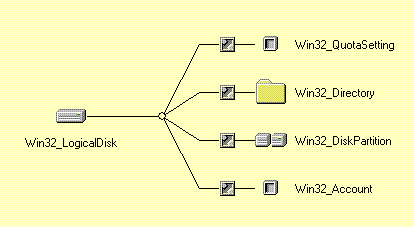
\includegraphics[width=0.8\textwidth]{afbeeldingen/Logical_Disk_association.png}
\end{figure}

Er wordt dus geen rekening gehouden met de associatorklassen die via overerving beschikbaar zijn (via superklassen van hetzij de eindpuntklassen, hetzij de associatorklassen). Er zijn voor de klasse Win32\_LogicalDisk een zestigtal associatorklassen beschikbaar!
\par Als je voor een instantie van een klasse de derde tabpagina (Associations) aanklikt krijg je een volledig overzicht van alle instanties waaraan deze instantie geassocieerd is (ook via overerving). Bekijk dit voor een instantie van de klasse Win32\_LogicalDisk.
\par Om de grafische uitvoer te simplificeren, wordt enkel van de eindpunten van de associatie de naam of het objectpad getoond. Toch kan ook de naam van de associatorklasse, en zelfs de attribuutnamen van de verwijzende sleutel, selectief getoond worden, door de muis respectievelijk over het icoontje van de associatorklasse of over een verbindingslijn met dat icoontje te schuiven. Dubbelklikken op het icoon van de associatorklasse of van een willekeurig eindpunt verschuift de focus naar de corresponderende klasse of instantie. Dit laat toe om doorheen een volledig kluwen van via associaties naar elkaar verwijzende klassen en objecten te navigeren.
\begin{enumerate}[resume]
	\item Vertrek van de Win32-klasse die een directory beschijft. Zoek de associatorklasse die directories en hun submappen koppelt. Wat is de sleutel van die associatorklasse?
	Zoek ook de associatorklasse die directories koppelt aan een logische drive. Bepaal alle instanties van de laatste associatorklasse. Wat is de betekenis van de waarde voor de sleutelattributen voor die instanties?
	\begin{lstlisting}
De Win32-klasse voor een directory is "Win32_Directory". 
De associatorklasse "Win32_SubDirectory" koppelt een directory aan een 
subdirectory. De sleutel is samengesteld uit 2 attributen "GroupComponent" en
"PartComponent". 

De associatorklasse "Win32_LogicalDiskRootDirectory" koppelt een directory aan 
een logische drive. Deze klasse heeft dezelfde sleutelattributen en een 
beperkt aantal instanties. De waarde van de sleutelattributen van een 
instantie stelt het absolute objectpad voor van het object waarnaar 
gerefereerd wordt.
	\end{lstlisting}
\end{enumerate}
Alle associatorklassen hebben een \textit{samengestelde sleutel}, opgebouwd uit twee attributen. Elk attribuut verwijst naar het absolute objectpad van het object waarnaar gerefereerd wordt. Hoe de sleutelattributen genoemd worden is niet aan voorwaarden onderworpen: toch hanteert men dikwijls duidelijke generische identifiers als GroupComponent/PartComponent en Antecedent/Dependent.
\begin{enumerate}[resume]
	\item Wat is er bijzonder aan de verbinding gerealiseerd door de associatorklasse Win32\_DependentService? Wat stelt de verbinding voor ? Wat is de betekenis van het extra attribuut? Is dit ingevuld voor bepaalde instanties?
	\begin{lstlisting}
Dit is een "recursieve verbinding": 
-> de "Antecedent" en "Dependent" attributen verwijzen naar dezelfde soort 
klassen "Win32_BaseService".  

Het bepaalt de volgorde waarin bepaalde NT services of systeemdrivers moeten 
opgestart worden.

Het extra attribuut "TypeOfDependency" bepaalt de soort afhankelijkheid tussen 
services. Ze beschrijft dat de verbonden Service moet zijn voltooid (waarde=2), 
gestart (3) of niet gestart (4) om de service te laten werken.
Dit attribuut is echter nooit ingesteld.
	\end{lstlisting}
	\item Er zijn meerdere WMI klassen die de belangrijkste logische en fysieke eigenschappen in verband met schijfpartities  beschrijven. Ze zijn ook onderling verbonden met associatorklassen.\\
	Zoek deze klassen en de associatorklassen op en bepaal enkele belangrijke attributen van elke WMI klasse.
	\begin{lstlisting}
Zoek op "partition" en je vindt de WMI klasse "Win32_DiskPartition". 
In het tabblad "Associations" vind je de figuur:

Hierin vind je alle antwoorden op de vraag:
"Win32_LogicalDisk"    (DeviceID, FileSystem, Size, FreeSpace, MediaType, Compressed,... )
      \ Dependent
       |  "Win32_LogicalDiskToPartition"
      / Antecedent
"Win32_DiskPartition"  (DeviceID, PrimaryPartition, StartingOffset, ... )
      \ Dependent
       | "Win32_DiskDriveToDiskPartition"
      / Antecedent
"Win32_DiskDrive"    (DeviceID, Model, InterfaceType, TotalCylinders, TracksPerCylinder, SectorsPerTrack, ... )
	\end{lstlisting}
	\item Zoek in WMI CIM Studio de Win32-klasse die een netwerkverbinding representeert (zoek alle klassen die in hun naam network bevatten). Elke instantie komt overeen met een mogelijke netwerkverbinding.
	\par Open (met c://windows/system32/ncpa.cpl) de grafische interface voor netwerkverbindingen. Dit lukt enkel als je ingelogd bent als administrator op je PC. Met Properties/Eigenschappen kan je de details van een netwerkverbinding (bijvoorbeeld van eth0) verder bekijken. Via welke attributen van de corresponderende WMI-object wordt deze informatie ter beschikking gesteld ? Zoek in de WMI-klasse de Status van een bepaalde netwerkverbinding.
	\par Welke associaties zijn er? Zoek de associatorklassen en de corresponderende sleutelattributen op.\\
	Bekijk in het bijzonder de informatie op het Resources/Bronnen tabpagina (bekomen na indrukken van de Configure ) en de Internet Protocol (TCP/IP) Properties. Deze informatie vind je terug in een geassocieerde klasse.
	Zoek zoveel mogelijk informatie hierover op in WMI CIM Studio.
	\begin{lstlisting}
De WMI klasse "Win32_NetworkAdapter" stelt een netwerkverbinding voor.
Het attribuut "NetConnectionStatus" bevat de "Status" van een 
netwerkverbinding. Zoek in "Property Qualifiers" de betekenis op van de 
numerieke waarden.

Deze klasse is o.a. geassocieerd met de configuratie-klasse, met volgende 
informatie:

"Win32_NetworkAdapterConfiguration" (Index, IPAddress, DHCPEnabled, DNSServerSearchOrder, ...)
     \ Setting
      | "Win32_NetworkAdapterSetting"
     / Element
"Win32_NetworkAdapter" (DeviceID, NetConnectionID, NetConnectionStatus,AdapterType, MACAddress, ... )


De informatie uit het "Resources"-tabblad is iets gecompliceerder, omdat ze 
overgeerfd wordt van de klasse "CIM_LogicalDevice". Vraag eerst alle 
instanties van de klasse "Win32_NetworkAdapter", en zoek de instantie die de 
netverbinding ("eth0)" voorstelt. Nu kan je voor die instantie alle 
geassocieerde klassen bekijken. 
Je vindt er meerdere koppelingen over de associatieklasse 
"Win32_AllocatedResource" die de informatie bevat van het "Resources"-tabblad. 

Je kan ook nagaan dat de klasse "Win32_NetworkAdapter", als subklasse van 
"CIM_LogicalDevice", gekoppeld is aan de klasse "CIM_SystemResource" via de 
associatorklasse is "Win32_AllocatedResource".


"Win32_NetworkAdapter" (-> subklasse van "CIM_LogicalDevice")
     \ Dependent
      | "Win32_AllocatedResource"
     / Antecedent
Win32-subklassen van "CIM_SystemResource":
"Win32_DeviceMemoryAddress" (StartingAddress, EndingAddress, Name, ....)
"Win32_PortResource"        (StartingAddress, EndingAddress, Name, ....)
"Win32_DMAChannel"          (DMAChannel attribuut)
"Win32_IRQResource"         (IRQNumber attribuut)	
	\end{lstlisting}
	\item Selecteer in WMI CIM Studio het object dat met de C: partitie van de harde schijf overeenstemt. Navigeer via Associations tabpagina's naar het object dat de eigenaar van het bestand c:/perl/bin/perl.exe representeert. Vermeld hierbij via welke associatorklassen (en de corresponderende sleutelattributen hiervan) je telkens gebruik maakt. Soms kan het vrij lang duren voor je de associaties te zien krijgt. Welke van die associatorklassen representeren recursieve verbindingen ?
	\begin{lstlisting}

Win32_LogicalDisk.DeviceID="C:"
     \ GroupComponent
      | Win32_LogicalDiskRootDirectory
     / PartComponent
Win32_Directory.Name="c:\\"
     \ GroupComponent
      | Win32_SubDirectory (recursief !)
     / PartComponent
Win32_Directory.Name="c:\\perl"
     \ GroupComponent
      | Win32_SubDirectory (recursief !)
     / PartComponent
Win32_Directory.Name="c:\\perl\\bin"
     \ GroupComponent
      | CIM_DirectoryContainsFile
     / PartComponent
CIM_DataFile.Name="c:\\perl\\bin\\perl.exe"
     \ Element
      | Win32_SecuritySettingOfLogicalFile
     / Setting
Win32_LogicalFileSecuritySetting.Path="c:\\perl\\bin\\perl.exe"
     \ SecuritySetting
      | Win32_LogicalFileOwner 
     / Owner
Win32_SID.SID="S-1-5-32-544"
     \ Setting
      | Win32_AccountSID 
     / Element
Win32_Group.Domain="computernaam",Name="Administrators"
	\end{lstlisting}
\end{enumerate}
\section{WMI Query Language (WQL)}

Consumers kunnen een specifiek WMI object/klasse opvragen door het opgeven van het absolute pad. Een consumer kan echter ook alle objecten/klassen opvragen die aan bepaalde criteria voldoen, op een analoge manier als in een relationele databankomgeving. De querytaal die men hierbij moet hanteren, de WMI Query Language (WQL), is gemodelleerd op een gereduceerde vorm van SQL, aangevuld met enkele WMI specifieke clausules. WQL ondersteunt geen join operaties. De syntax van deze beperkte querytaal kan je terugvinden in de subtakken van de WMI-documentatie: WMI Reference / WMI and SQL / WQL (SQL for WMI).
\par Je kan een WQL query opvragen in WMI CIM Studio met de drukknop in de het rechterpaneel. Je kan ook WbemTest gebruiken. Na connectie met de namespace vraag je een Query.
\subsection{Zoek instanties van een bepaalde klasse}
De eenvoudigste WQL query haalt alle instanties op van één klasse, die aan bepaalde voorwaarden voldoen:
\begin{lstlisting}
SELECT * FROM klassenaam [WHERE ...]
\end{lstlisting}
De FROM clausule bevat de klassenaam als enig argument. Zonder WHERE clausule resulteert deze WQL query in een lijst met alle instanties van de opgegeven klasse (of tot een klasse die ervan afgeleid is). In deze WQL query worden alle attributen opgehaald van de objecten die voldoen. Je kan het *-teken vervangen door een lijst van attributen (projectie) maar dat wordt meestal niet gedaan.
\begin{enumerate}[resume]
	\item Bepaal met een WQL query alle instanties van de klasse CIM\_LogicalDisk.
	Bepaal ook alle instanties van Win32\_OperatingSystem. Merk op dat je hier niet moet weten of deze klasse een singleton-klasse is.
	\begin{lstlisting}
SELECT * FROM Win32_CIM_LogicalDisk 
SELECT * FROM Win32_OperatingSystem 
	\end{lstlisting}
\end{enumerate}
Indien er veel objecten voldoen aan de WQL query (vb alle directories), dan krijg je problemen. In WMI CIM Studio blokkeert de applicatie, in WbemTest wordt maar een beperkt aantal objecten opgehaald. Je kan dit best oplossen door met een WHERE predicaat de lijst zelf te verkleinen.
In elementaire WHERE predicaten mogen enkel vergelijkingsoperatoren ($=$,$!=$,$<>$,$<$,$<=$,$>$ of $>=$), de (NOT) LIKE en de IS (NOT) NULL operatoren gebruikt worden. (niet alle types ondersteunen deze vergelijkingsoperatoren !)
\par Net zoals in SQL kan men eenvoudige predicaten willekeurig samenstellen met behulp van de logische operatoren AND, OR en NOT, en met ronde haakjes de evaluatievolgorde van predicaten aanpassen. Als de 'waarden' die je gebruikt in de WHERE predicaten van het type string zijn moet je "" of '' toevoegen. Bovendien moet je in de WHERE clausule alle backslashen backslashen.
\par In de SELECT en WHERE clausules mag men ook systeemattributen opnemen: zo kan men bijvoorbeeld met behulp van \_\_CLASS het resultaat beperken tot objecten die strikt tot de in de FROM clausule opgegeven klasse behoren, en niet tot een klasse die ervan afgeleid is.
Let op! je kan GEEN beperking opleggen op de qualifiers van de klasse, enkel op de attributen.
\begin{enumerate}[resume]
	\item Bepaal alle partities op de computer.
	Bepaal daarna alle opslagelementen (subklassen van CIM\_StorageExtent) die geen partitie voorstellen.
	\begin{lstlisting}
#alle partities
SELECT * FROM Win32_LogicalDisk

#alle opslagelementen, geen partities - let op de ''-tekens
SELECT * FROM CIM_StorageExtent  WHERE  __CLASS != 'Win32_LogicalDisk'
	\end{lstlisting}
	\item De rootdirectory van de C:partitie is een instantie van Win32\_Directory. Het lukt niet om alle instanties van die klasse te vragen! Je kan wel eerst de Win32\_LogicalDisk ophalen die hoort bij de C:-drive, en dan via het Associations tabpagina dit object terugvinden.\\
	Een WQL-query is een zinvol alternatief om toch direct de rootdirectory te connecteren. Stel de WQL-query op die de rootdirectory van de C:partitie direct ophaalt.
	\begin{lstlisting}
De rootdirectory die bij de C:partitie hoort

SELECT * FROM Win32_Directory WHERE name="c:\\"
of
SELECT * FROM Win32_Directory WHERE name='c:\\'

Je gebruikt best het sleutelattribuut om de instantie te beschrijven. 
Je mag de ' ' of " "-tekens niet weglaten, en backslashen backslashen !

Opmerking: Beide WMI-objecten zijn aan elkaar geassocieerd via de 
associatorklasse Win32_LogicalDiskRootDirectory. Deze associatorklasse 
direct ophalen lukt niet omdat de enige attributen een reference-type 
hebben.
	\end{lstlisting}
	\item Zoek met een WQL-query alle processen die ofwel minimaal 10 MB geheugenruimte innemen, ofwel voldoen aan de 2 voorwaarden: ze hebben meer schrijf- dan leesbewerkingen uitgevoerd en ze worden door minstens 10 threads ondersteund.
	\begin{lstlisting}
SELECT *
FROM   Win32_Process
WHERE  Workingsetsize > 10000000
OR  (WriteOperationCount > ReadOperationCount
And ThreadCount >= 10)

Je kan ook een lijst met gewenste attributen opgeven, maar dat heeft geen 
effect op de performantie:
SELECT Name,Workingsetsize,WriteOperationCount,ReadOperationCount,ThreadCount ....
	\end{lstlisting}
	\item Zoek eerst in WMI CIM Studio welke WMI klasse kan gebruikt worden om een ping - opdracht uit te voeren. In welk attribuut kan je het ip-adres opgeven, welk attribuut bevat informatie over het antwoord van deze request?\\
	Stel nu een WQL query op die een ping-opdracht aanvraagt naar het adres 'google.com' (in de WHERE clausule). Bekijk het antwoord van deze ping request.
	\begin{lstlisting}
Zoek de WMI-klasse met "Search for Class" waarbij je zoekt naar een klasse of 
attribuut dat "ping" bevat.

Merk op dat je in WMI CIM Studio geen instanties kan vragen van deze klasse. 

WQL-query:
SELECT ResponseTime,StatusCode FROM Win32_PingStatus WHERE Address='google.com'
	\end{lstlisting}
\end{enumerate}
\subsection{Zoek klassen in de CIM repository}
WQL kan ook gebruikt worden om de klassedefinities in de CIM repository op te vragen. Hiermee kan je klassen opzoeken die aan bepaalde criteria voldoen. Dergelijke queries worden \textbf{schemaqueries} genoemd.
Een schemaquery haalt enkel klassen op uit de namespace waaraan je geconnecteerd bent:
\begin{lstlisting}
SELECT * FROM meta_class [WHERE ...]
\end{lstlisting}
Zonder WHERE clausule haal je dus álle klassen op uit de namespace waaraan je geconnecteerd bent.
Als je een schemaquery uitvoert in WbemTest wordt de bovenliggende klasse ook getoond in het resultscherm.
\begin{enumerate}[resume]
	\item Is het mogelijk om met één WQL query alle abstracte klassen op te halen ? Is het mogelijk om met één WQL query alle associatorklassen op te halen ?
	\begin{lstlisting}
Je kan in de WHERE clausule geen qualifiers gebruiken, en deze informatie is 
enkel opgeslagen in de klassequalifier abstract
Ook de eigenschap of een klasse een associatorklasse is wordt in een 
klassequalifier opgeslagen, en kan dus niet worden gespecifieerd in een 
WQL query.
	\end{lstlisting}
	\item Stel telkens een WQL query op voor volgende resultaatset:
	\begin{itemize}
		\item enkel de CIM\_Service klasse,
		\begin{lstlisting}
SELECT * FROM meta_class
WHERE __CLASS = 'CIM_Service'
		\end{lstlisting}
		\item alle klassen die onmiddellijk van CIM\_Service afgeleid zijn (zoek eerst het systeemattribuut dat de bovenliggende klasse bevat),
		\begin{lstlisting}
SELECT * FROM meta_class
WHERE __SUPERCLASS = "CIM_Service"
		\end{lstlisting}
		\item alle klassen die niet van een andere klasse afgeleid zijn (lukt enkel in WbemTest)
		\begin{lstlisting}
SELECT * FROM meta_class
WHERE __SUPERCLASS IS null
		\end{lstlisting}
	\end{itemize}	
\end{enumerate}
In schemaqueries kan je in de WHERE clausule gebruik maken van het sleutelwoord \_\_THIS (verwijst naar één klasse in de resultaatset), in combinatie met de ISA operator:
\begin{lstlisting}
WHERE __THIS ISA 'klassenaam'
\end{lstlisting}
Dit beperkt de lijst tot alle klassen die afgeleid zijn van de opgegeven klasse. Ook hier zijn de ' '-tekens noodzakelijk.
\begin{enumerate}[resume]
	\item Bepaal alle klassen die rechtstreeks of onrechtstreeks van CIM\_Service afgeleid zijn, met uitzondering van zichzelf.
	\begin{lstlisting}
SELECT * FROM meta_class
WHERE __THIS ISA 'CIM_Service'
AND __CLASS != 'CIM_Service'
	\end{lstlisting}
\end{enumerate}
\subsection{Extra mogelijkheden met WQL}
Omdat WQL geen join-operaties ondersteunt is het niet evident om alle objecten op te halen die via associatorklassen aan een specifieke objectinstantie gelinkt zijn.
Er is wel voorzien in een oplossing hiervoor: vervang de SELECT * FROM opdracht door een \textbf{REFERENCES OF {…}} of een \textbf{ASSOCIATORS OF {…}} opdracht. Tussen de akkolades moet een relatief objectpad van een doelobject worden opgegeven - zoek het juiste relatief pad vooraf op zodat je geen fout krijgt.
\begin{itemize}
	\item REFERENCES OF {…} achterhaalt alle instanties van associatorklassen die direct of indirect verbonden zijn met het doelobject
	\item ASSOCIATORS OF {…} bepaalt alle instanties van reguliere klassen die gelinkt zijn aan het doelobject, dus alle eindpunten van de associaties.
\end{itemize}

Let op! Aangezien hier enkel instanties worden opgehaald zal de resultset leeg zijn indien je voor het doelobject een klasse opgeeft.
Vooral de laatste clausule is interessant. We beperken de oefeningen dan ook tot deze clausule.
\par Zonder WHERE clausule (zie verder) levert een ASSOCIATORS OF opdracht alle objecten op, van om het even welke klasse, die via om het even welke associatorklasse met het doelobject verbonden zijn. Dit geeft een analoog resultaat als de output verkregen met WMI CIM Studio in de Associations tabpagina van het detailpaneel van het doelobject.
\par Let op! De syntax van dit soort WQL-query's is niet helemaal dezelfde als voor de SELECT-clausule. Als het objectpad (van het type string) een backslash en " bevat dan moet je de backslash backslashen, tenzij je " vervangt door ', dan behoud je de enkele backslash (zie volgende voorbeeld)
\begin{enumerate}[resume]
	\item Alle objecten die geassocieerd zijn met de rootdirectory van de C:partitie kan je opvragen in het tabblad Associations van het bijhorend object Stel een WQL query op die hetzelfde overzicht geeft.
	\begin{lstlisting}
ASSOCIATORS OF {Win32_Directory.Name="c:\\"}   #het relatief objectpad dat je in CIM Studio terugvindt

Let op, je MOET "" gebruiken dus onderstaande WQL-query resulteert in een foutmelding:
ASSOCIATORS OF {Win32_Directory.Name='c:\\'}

Lukt wel:
ASSOCIATORS OF {Win32_Directory.Name='c:\'}
	\end{lstlisting}
\end{enumerate}
Er kan ook een \textit{WHERE clausule} worden toegevoegd, maar deze heeft een \textit{compleet andere bedoeling, en ook een andere syntax}! Meer informatie in de WMI-documentatie.
\par In de WHERE clausule kan je één of meerdere "predicaten" toevoegen, die telkens een \textit{beperking opleggen aan de resultaten}. Alle predicaten moeten hierbij simultaan vervuld worden (de AND operator wordt impliciet verondersteld, en mag men niet vermelden). Hieronder de meest interessante predicaten.
\par Volgende predicaten leggen een extra voorwaarde op aan de objecten die opgehaald worden:
\begin{itemize}
\item \textbf{AssocClass} = klassenaam: enkel objecten die via de vermelde associatorklasse met het doelobject verbonden zijn,
\item \textbf{ResultClass} = klassenaam: enkel objecten die behoren tot de vermelde klasse,
\item \textbf{ResultRole} = sleutelattribuutnaam (van een associatorklasse): enkel objecten die via associaties zijn bekomen waarbij in het vermelde sleutelattribuut verwezen wordt naar een objectpad van het eindpunt,
\item \textbf{Role} = sleutelattribuutnaam (van een associatorklasse): enkel objecten die via associaties zijn bekomen waarbij in het vermelde sleutelattribuut verwezen wordt naar een objectpad van het doelobject.
\end{itemize}
De laatste twee predicaten zijn in het bijzonder nuttig bij recursieve associaties.
\par Er zijn twee predicaten waarmee je klasse-definities vraagt, en geen instanties.
\begin{itemize}
\item \textbf{SchemaOnly}: gebruik je als het doelobject zelf een klasse is (dit predicaat ontbreekt bij de beschrijving van ASSOCIATORS OF in de MSDN Library)
\item \textbf{ClassDefsOnly}: gebruik je als het doelobject een instantie is.
\end{itemize} 
\begin{enumerate}[resume]
	\item Pas vorig overzicht aan zodat enkel de geassocieerde klassen getoond worden in plaats van alle instanties.
	\begin{lstlisting}
ASSOCIATORS OF {Win32_Directory.Name="c:\\"} WHERE ClassDefsOnly 
	\end{lstlisting}
	\item Bepaal in 3 stappen, met opeenvolgende WQL queries, het totaal aantal sectoren van de schijf van C:\verb+\+ partitie.
	Vertrek hierbij van de rootdirectory C:\verb+\+\verb+\+ van deze partitie, en gebruik onderstaande associaties om tot de gewenste attribuut Totalsectors te gaan.
	\begin{lstlisting}
Win32_Directory   (Name="C:\\")
      \ 
       | Win32_LogicalDiskRootDirectory
      / 
Win32_LogicalDisk   
      \ 
       | Win32_LogicalDiskToPartition
      / 
Win32_DiskPartition 
      \ 
       | Win32_DiskDriveToDiskPartition
      / 
Win32_DiskDrive      (TotalSectors)
	\end{lstlisting}
	\begin{lstlisting}
We vertrekken van het WMI-object Win32_Directory.Name="c:\\"

ASSOCIATORS OF {Win32_Directory.Name="c:\\"} 
WHERE ResultClass=Win32_LogicalDisk

-> WMI-object: Win32_LogicalDisk.DeviceID="C:"

ASSOCIATORS OF {Win32_LogicalDisk.DeviceID="C:"}
WHERE ResultClass = Win32_DiskPartition

-> WMI-object: Win32_DiskPartition.DeviceID="Disk #0, Partition #1"

ASSOCIATORS OF {Win32_DiskPartition.DeviceID="Disk #0, Partition #1"}
WHERE ResultClass = Win32_DiskDrive

->bevat het attribute TotalSectors
	\end{lstlisting}
	\item epaal door opeenvolgende WQL queries het MAC-adres, het IP-adres en het interruptnummer dat aan de eth0 kaart is gekoppeld. Zoek zelf de WMI-klassen die deze informatie bevatten
	\begin{lstlisting}
SELECT DeviceID,MACAddress FROM Win32_NetworkAdapter          
WHERE NetConnectionID="eth0"                               //MAC-adres

ASSOCIATORS OF {Win32_NetworkAdapter.DeviceID="9"}
WHERE ResultClass = Win32_NetworkAdapterConfiguration      //IP-adres

ASSOCIATORS OF {Win32_NetworkAdapter.DeviceID="9"}       
WHERE ResultClass = Win32_IRQResource                      //interruptnumber 
	\end{lstlisting}
	\item Beschouw de map c:/perl/lib. Aan welke klassen is dit object geassocieerd ? Bepaal via WQL queries achtereenvolgens:
	\begin{itemize}
		\item alle bestanden in deze map,
		\begin{lstlisting}
ASSOCIATORS OF {Win32_Directory.Name='c:\perl\lib'}  WHERE ResultClass = CIM_DataFile
		\end{lstlisting}
		\item alle submappen van deze map,
		\begin{lstlisting}
twee mogelijkheden:

ASSOCIATORS OF {Win32_Directory.Name='c:\perl\lib'}  WHERE ResultClass = Win32_Directory
Role = GroupComponent

ASSOCIATORS OF {Win32_Directory.Name='c:\perl\lib'}  WHERE ResultRole = PartComponent
		\end{lstlisting}
		\newpage
		\item de map waarvan c:/perl/lib een submap is.
		\begin{lstlisting}
twee mogelijkheden:

ASSOCIATORS OF {Win32_Directory.Name='c:\perl\lib'}
WHERE ResultRole = GroupComponent

ASSOCIATORS OF {Win32_Directory.Name='c:\perl\lib'}
WHERE ResultClass = Win32_Directory
Role = PartComponent
		\end{lstlisting}
	\end{itemize}	
\end{enumerate}
Enkel met de clausule \textit{WHERE schemaonly}, kan je voor het argument een klassenaam opgeven in plaats van een objectpad van een instantie. Men krijgt dan precies hetzelfde resultaat als verkregen met WMI CIM Studio in de Associations tabpagina van het detailpaneel van de klasse.
\begin{enumerate}[resume]
	\item Bepaal alle klassen die kunnen geassociëerd worden aan een Directory, zonder rekening te houden met overerving.
	\begin{lstlisting}
ASSOCIATORS OF {Win32_Directory} WHERE schemaonly 
	\end{lstlisting}
\end{enumerate}
\subsection{Notification queries}
Voor deze oefeningen moet je \textit{inloggen als administrator}, met volledige rechten.
Net zoals SNMP ondersteunt WMI niet alleen externe polling, waarbij de consumer telkens opnieuw het initiatief moet nemen, maar ook het \textit{equivalent van een trap mechanisme}: event notification. Het ideale scenario hier is dat de provider zelf meldt dat een gebeurtenis is opgetreden waarin één of andere consumer zich heeft geregistreerd (a priori gemeld heeft geïnteresseerd te zijn). Dit gebeurt door het creëren van een objectinstantie in één van de subklassen van de \_\_Event systeemklasse. Enkel wanneer de corresponderende voorwaarden vervuld zijn, wordt de consumer geactiveerd om te reageren op het event. Zolang het event niet optreedt, hoeven noch de consumers, noch de WMI service processortijd te besteden aan het monitoren van de voorwaarden.

De registratie van een event gebeurt met behulp van WQL syntax, en wordt een \textit{Notification Query} genoemd. Informatie in verband met Notification Queries kan je terugvinden in de Using WMI / Supporting Tasks for WMI / Querying with WQL / Receiving Event Notification subtak van de WMI-documentatie. Het uittesten ervan kan niet in WMI CIM Studio, maar lukt wel in het WbemTest hulpprogramma: na connectie met een namespace, vink je Asynchronous aan in het Method Invocation Options vak, druk je op de knop Notification Query. Het is nu belangrijk dat je een WQL query opgeeft, die een \_\_Event-klasse analyseert. Als je een gewone WQL query opgeeft dan resulteert dit in een fout. De notification query heeft als basis-syntax
\begin{lstlisting}
SELECT * FROM Eventklasse 
\end{lstlisting}
In WbemTest worden alle instanties getoond van de gevraagde Eventklasse. In een volgend labo zullen we dan zelf een gewenste 'actie' toevoegen.

\begin{enumerate}[resume]
	\item Er zijn meerdere Eventklassen (subklassen van de \_\_Event klasse) waarin events kunnen gegenereerd worden. Zoek deze klassen op in WMI CIM Studio.
	Met welke gewone WQL query vraag je alle \_\_Event klassen van de geconnecteerde namespace op.\\
	Let op! Dit is een gewone query, en nog geen notification query.
	\begin{lstlisting}
select * from meta_class  where __THIS ISA '__Event'
	\end{lstlisting}
	\item Eenvoudig voorbeeld met \textbf{periodieke events}: De klasse \_\_TimerEvent wordt gebruikt om periodieke taken te initialiseren. Je kan periodiek \_\_TimerEvent objecten laten aanmaken met behulp van een \_\_TimerInstruction object. Creeer in WMI CIM Studio, een \_\_IntervalTimerInstruction object dat elke minuut een \_\_TimerEvent aanmaakt (opgelet: het IntervalBetweenEvents attribuut wordt uitgedrukt in milliseconden !) (enkel voor administrator).\\
	Maak nu in WbemTest een notificaton query die reageert op events van de eventklasse \_\_TimerEvent.\\
	Van zodra een \_\_TimerEvent optreedt, verschijnt een popup venster waarin je de oorzaak van het event kan analyseren.
	\begin{lstlisting}
SELECT * FROM __TimerEvent
	\end{lstlisting}
	\item Construeer een notification query die een event genereert telkens de notepad toepassing opgestart of afgesloten wordt. Zoek eerst op welk soort object wordt aangemaakt/verwijdert bij het opstarten van notepad ?\\
	Zoek in WMI CIM Studio de juiste subklasse van \_\_ExtrinsicEvent.
	\begin{lstlisting}
SELECT * FROM Win32_ProcessTrace WHERE ProcessName = 'notepad.exe'
	\end{lstlisting}
\end{enumerate}
Alhoewel in de specificaties voor de ontwikkeling van providers aangedrongen wordt op het ondersteunen van deze functionaliteit, zijn er momenteel slechts een b\textit{eperkt aantal }providers (ondermeer de Event Log, provider) die ook deze event provider functie implementeren, en specifieke \_\_EVENT-klassen voorzien.
\par Gelukkig is er hier een generische \textit{tussenoplossing}, die externe polling door de consumers toch kan vermijden. Deze oplossing, die het best als \textbf{interne polling} kan omschreven worden, komt er op neer dat de WMI service periodiek de toestand van specifieke objecten bij de corresponderende providers opvraagt en vergelijkt.
\par Het registreren in, en het verwerken van een event is voor een consumer nagenoeg eender, of het event gecreeerd werd door een event provider, of door interne polling door de WMI service. In de WMI-documentatie vind je ook extra informatie over de eventklassen in de tak WMI Reference / WMI Classes / WMI System Classes.
De meest interessante eventklassen zijn de subklassen van de InstanceOperationEvent klasse. Zoek volgende klassen op, zowel in de WMI-documentatie als in WMI CIM Studio:
\begin{itemize}
	\item \textbf{InstanceCreationEvent} en \textbf{InstanceDeletionEvent}, die respectievelijk gecreeerd worden bij creatie of verwijdering van een specifiek doelobject. Deze klassen hebben twee interessante attributen: \textit{TIME\_CREATED} en \textit{TargetInstance}. Dit laatste attribuut is een embedded object waarvan de attributen precies zijn ingevuld met de gegevens van het doelobject op het ogenblik van de creatie of de verwijdering ervan.
	\item \textbf{InstanceModificationEvent}, het gevolg van specifieke wijzigingen van de attributen van een doelobject. Nu is behalve een \textit{TargetInstance} ook een \textit{PreviousInstance} attribuut beschikbaar. Zowel de attributen voor als na de wijziging van het doelobject kunnen bijgevolg gerecupereerd worden.
\end{itemize}

\par Bij interne polling wordt dus een \textit{snapshot techniek} gehanteerd. De voorlaatste en de laatste snapshots worden, indien beschikbaar, de PreviousInstance en de TargetInstance genoemd. Op basis van de vergelijking van de attributen van beide snapshots wordt dan eventueel een eventobject (een instantie van een subklasse van \_\_Event) gecreëerd.
\par Indien van het interne pollingmechanisme moet gebruik gemaakt worden (in de meeste gevallen !), dan moet \textit{de pollingperiode (uitgedrukt in seconden) met behulp van de WITHIN … extentie aan de FROM clausule toegevoegd worden}. Je kan in WbemTest proefondervinderlijk vaststellen of dit nodig is: ontbreekt een noodzakelijke WITHIN … extentie, dan krijg je een gepaste foutcode (0x80042002).
\par Om overbelasting tegen te gaan zal je best altijd verder specifiëren welke klasse de event veroorzaakt. Hiervoor neem je in de WHERE clausule minstens één predicaat op die verwijst naar de klasse van het doelobject. Welke acties moet je ondernemen om events te laten genereren voor:
\begin{lstlisting}
SELECT * FROM __InstanceModificationEvent Within 5
WHERE TargetInstance ISA 'Win32_Service'
\end{lstlisting}
Met het TargetInstance attribuut beschik je over het doelobject, en kan je met behulp van de ISA operator de klasse van dit doelobject vergelijken met de gewenste klasse (WHERE TargetInstance ISA 'Klassenaam').
\par In andere predikaten van de WHERE clausule wordt meestal ook verwezen naar de attributen van de TargetInstance snapshot, of van de PreviousInstance snapshot. Dit kan door een gequalificeerde syntax (bijvoorbeeld TargetInstance.attribuutnaam) te hanteren.
\par Indien je te weinig beperkingen oplegt aan de WQL-query kan het systeem blokkeren.
\begin{enumerate}[resume]
	\item Construeer een notification query die een event genereert telkens een Windows service zijn Running toestand verliest (of dit veroorzaakt wordt door de service netjes te stoppen, of door het corresponderend proces abrupt af te breken, maakt niet uit).
	\begin{lstlisting}
SELECT * FROM __InstanceModificationEvent Within 5
WHERE TargetInstance ISA 'Win32_Service'
And PreviousInstance.Started = true
And TargetInstance.Started   = false
	\end{lstlisting}
	\newpage
	\item Je kan oefening 33 ook oplossen zonder interne polling, door enkel gebruik te maken van de algemene event-klassen. De voorwaarde wordt wel iets complexer.
	\begin{lstlisting}
#Met interne polling - zonder extrinsic event:

SELECT * FROM __InstanceOperationEvent Within 10
WHERE TargetInstance ISA 'Win32_Process'
And TargetInstance.Name = 'notepad.exe'
And (__CLASS = '__InstanceCreationEvent'
Or __CLASS = '__InstanceDeletionEvent')
	\end{lstlisting}
	\item Construeer een notification query die een event genereert telkens in een specifieke directory (bijvoorbeeld c:/temp) een bestand gecreëerd wordt. Los deze vraag op twee manieren op, telkens vertrekkend van een andere WMI klasse.
	\begin{lstlisting}
Twee oplossingen:

SELECT * FROM __InstanceCreationEvent Within 10
WHERE TargetInstance ISA 'CIM_DirectoryContainsFile'
And TargetInstance.GroupComponent = "Win32_Directory.Name='c:\\temp'" 
#let op het gebruik van "" en '' 

Alternatief: een bestand staat in een bepaalde map als de drive en het pad 
overeenkomen met de directory:

SELECT * FROM __InstanceCreationEvent Within 10
WHERE TargetInstance ISA 'CIM_DataFile'
And TargetInstance.Drive = 'c:'
And TargetInstance.Path = '\\temp'

Lukt ook met:
SELECT * FROM __InstanceCreationEvent Within 10
WHERE TargetInstance ISA 'CIM_DataFile'
And TargetInstance.Drive = "c:"
And TargetInstance.Path = "\\temp"
	\end{lstlisting}
\end{enumerate}
WQL ondersteunt, enkel bij een notification query, de GROUP WITHIN clausule, met een aantal optionele extenties. GROUP WITHIN wordt gevolgd door een tijdsperiode, uitgedrukt in seconden. Indien deze clausule gebruikt wordt, veroorzaakt niet elke gebeurtenis die aan de voorwaarden voldoet een \_\_Event object. In de plaats hiervan wordt per periode hoogstens één \_\_AggregateEvent object gegenereerd. Dit vermijdt dat het systeem overbelast wordt door events die te frequent optreden. De periode van de GROUP WITHIN clausule is typisch een veelvoud van de periode vermeld in de WITHIN … extentie (voor zover die vereist is) van de FROM clausule.
\par Het \textit{NumberOfEvents} attribuut van het \_\_AggregateEvent object telt hoeveel gebeurtenissen er effectief opgetreden zijn. Het Representative attribuut verwijst naar één van deze gebeurtenissen. De informatie in verband met de andere gebeurtenissen uit de periode gaat verloren.
\newpage
\par De optionele \textit{BY} extentie, gevolgd door een attributenlijst, laat toe om in de periode een \_\_AggregateEvent object te genereren voor elke unieke combinatie van de attributen in de lijst. 
\par De optionele \textit{HAVING} NumberOfEvents … extentie laat toe om drempelwaarden op te leggen aan het aantal gebeurtenissen in de periode. Worden deze drempelwaarden niet bereikt, dan wordt ook geen \_\_AggregateEvent object gecreëerd.
\begin{enumerate}[resume]
	\item In een specifieke directory (bijvoorbeeld c:\verb+\+temp) kunnen zowel bestanden als submappen gecreëerd worden. Ontwikkel een notification query die per periode (bijvoorbeeld elke minuut) maximaal twee events genereert: één event groepeert de nieuwe bestanden, een ander event groepeert de nieuwe submappen. Bekijk in WbemTest de attributen van het \_\_AggregateEvent
	\begin{lstlisting}
SELECT * FROM __InstanceCreationEvent WITHIN 5
WHERE TargetInstance.GroupComponent = "Win32_Directory.Name='c:\\temp'"
AND (TargetInstance ISA 'CIM_DirectoryContainsFile'
OR TargetInstance ISA 'Win32_SubDirectory')
GROUP BY TargetInstance.__CLASS WITHIN 60 
	\end{lstlisting}
\end{enumerate}
\subsection{Permanente eventregistratie}
In de voorgaande methode kan je enkel zien dat er een \_\_Event object wordt aangemaakt. In de volgende labo's zal aan een event ook een bepaalde "actie" gekoppeld worden. Er bestaat ook een tweede manier, waarbij \textit{de gewenste actie wordt opgeslaan in een klasse}. Hiervoor beschik je over de \textbf{Eventconsumer-klassen}, die een actie kan beschrijven
Na een standaard WMI installatie worden dikwijls in de belangrijkste namespaces een vijftal configureerbare eventconsumers geregistreerd. Op de labotoestellen is dit reeds gebeurd in de root/cimv2 namespace. Zoek in WMI CIM Studio de volgende klassen op:
\begin{itemize}
\item de \textbf{LogFileEventConsumer} laat toe om detailinformatie van een gebeurtenis te loggen in een tekstbestand. Indien voor een bestand met een maximale grootte gekozen wordt, dan wordt automatisch een systeem toegepast met roterende bestandsnamen (met een numerieke suffix).
\item de \textbf{NTEventLogEventConsumer} doet net hetzelfde, maar gebruikt de EventLog van Windows in plaats van een tekstbestand.
\item de \textbf{SMTPEventConsumer} laat toe om na een specifieke gebeurtenis een volledig configureerbare email te sturen.
\item de \textbf{CommandLineEventConsumer} kan een gebeurtenis laten volgen door de uitvoering van een willekeurig programma, geparametriseerd door detailattributen van de gebeurtenis, die bijvoorbeeld als argumenten bij de uitvoeringsopdracht van het programma kunnen worden meegegeven.
\item de \textbf{ActiveScriptEventConsumer} kan bij een specifieke gebeurtenis een script laten uitvoeren, bijvoorbeeld een WMI consumerscript. In het kader van deze labo's ligt de keuze voor PerlScript als programmeertaal voor de hand.
\end{itemize}
Om eventueel ook thuis deze EventConsumer-klassen te registreren heb je de bestanden scrcons.mof, smtpcons.mof en wbemcons.mof nodig (voer in Vista of Windows Server 2008 eerst een download uit van deze bestanden, ter vervanging van de in de directory\\ \verb+\+WINDOWS\verb+\+system32\verb+\+wbem standaard geïnstalleerde bestanden). Zorg ervoor dat de oude bestanden worden overschrijven - indien dit niet lukt dan moet je de toegangseigenschappen aanpassen (zie theorie). \\Je voert éénmalig de volgende commando's uit (als administrator):
\begin{lstlisting}
mofcomp scrcons.mof
mofcomp smtpcons.mof
mofcomp wbemcons.mof
\end{lstlisting}
Meer gedetailleerde informatie over deze klassen vind je terug in de WMI Reference / WMI Classes / Standard Consumer Classes subtak van de WMI-documentatie. De eerste vier consumers uit de verzameling laten toe om, louter met behulp van WMI CIM Studio, te reageren op interessante gebeurtenissen. Aangezien de configuratie van deze eventconsumers gebeurt op basis van instanties van statische klassen, wordt deze permanent in de CIM repository opgeslagen, en moet ze dan ook maar éénmalig gebeuren. De eventconsumers worden geactiveerd van zodra de WMI service opgestart wordt. Na herbooten van het toestel moet er dan ook geen enkele extra handeling gebeuren. 
\par Deze eenvoudige vorm van permanente eventregistratie kan in de praktijk instaan voor een groot deel van beheersaspecten waarvoor een event mechanisme aangewezen is. In principe is het ook mogelijk om zelf meer specifieke consumers te ontwikkelen, die men vervolgens op een analoge manier kan gebruiken. Het ontwikkelen van een dergelijke consumer kan echter niet in een scripttaal, en heeft een moeilijkgraad die te hoog is voor deze labo's.

\par Om één van de hierboven vermelde standaard eventconsumers in WMI CIM Studio te configureren moeten drie objecten worden gemaakt:
\begin{figure}[h]
	\caption{Associatorklasse}
	\centering
	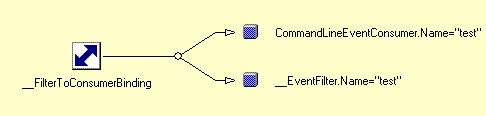
\includegraphics[width=0.8\textwidth]{afbeeldingen/PermanenteEventRegistratie.png}
\end{figure}

Er zijn twee objecten, die aan elkaar gekoppeld worden met een associator:
\begin{itemize}
	
	\item \textbf{\_\_EventFilter object}: hierin formuleer je de oorzaken die tot een event leiden. Naast het sleutelattribuut, moeten twee attributen worden ingesteld: QueryLanguage wordt ingevuld met WQL en Query wordt ingevuld met de WQL code van een notification query. Dit is dus een notification query die permanent wordt opgeslaan in een \_\_EventFilter object. Het is aangeraden om deWQL query voorafgaand uit te testen, bijvoorbeeld met behulp van WbemTest.
	\par Net als bij Notification queries zal automatisch een eventobject (\_\_Event of \_\_AggregateEvent) worden gemaakt telkens als het event optreedt. De attributen (TargetInstance, \_\_SERVER, NumberOfEvents, Representative, ... ) van het eventobject bevatten de relevante informatie van het event.
	\item \textbf{\_\_EventConsumer object} : beschrijft de reactie die je wenst op een event. Dit is een abstracte klasse, je moet verder kiezen : LogFileEventConsumer, NTEventLogEventConsumer, SMTPEventConsumer, CommandLineEventConsumer of ActiveScriptEventConsumer object. Afhankelijk van de specifieke \_\_EventConsumer klasse die gekozen werd, initialiseer je de reactie met behulp van de specifieke attributen. 
	\par Voor een CommandLineEventConsumer bijvoorbeeld is het CommandLineTemplate attribuut (de uit te voeren opdracht, inclusief argument) essentiëel, terwijl men bij een SMTPEventConsumer doorgaans minimaal de ToLine, FromLine, Subject, Message en SMTPServer argumenten invult.
	\item \textbf{\_\_FilterToConsumerBinding associatorobject} : realiseert de koppeling van het \_\_EventFilter object aan het \_\_EventConsumer object. Je vult enkel de 2 sleutelattributen Filter en Consumer in met de juiste referentie naar de objecten die je in de twee eerste stappen hebt aangemaakt. 
	\par Aangezien associatorklassen veel-op-veel verbindingen representeren, kan één event meerdere reacties teweegbrengen. Anderzijds kan men dezelfde consumer configureren als reactie op een aantal diverse bronnen. Handig hierbij is dat, indien een templatestring in de consumerinstantie verwijst naar een attribuut dat voor het optredende event niet van toepassing is, dit geen aanleiding geeft tot een fout. De template wordt in die situatie vervangen door een lege string.
\end{itemize}
Je moet deze drie objecten aanmaken, en ervoor zorgen dat de sleutelattributen de juiste inhoud hebben. Bovendien moet je een aantal attributen instellen die de gewenste actie zinvol maken.
\begin{enumerate}[resume]
	\item De eenvoudigste toepassing van het permanente eventregistratiemechanisme is het uitvoeren van periodieke taken. We vertrekken van het \_\_TimerInstruction object uit oefening 33 en bepalen nu de reactie de we wensen voor events van de klasse \_\_TimerEvent.
	\par De gewenste reactie is dat periodiek (elke minuut dus) de SNMP service opnieuw gestart wordt. Je kan dit realiseren via de commandline-opdracht net start snmp (volledige pad opgeven voor de opdracht). Indien de SNMP service reeds actief is, dan heeft een dergelijke opdracht geen enkel effect (behalve een onnodige belasting). Indien de SNMP service echter om één of andere reden niet actief zou zijn, dan wordt op die manier periodiek gepoogd dit te corrigeren.
	\\De opdracht die je vraagt wordt opgestart in embedded mode, en kan je dus nooit "zien".
	\begin{lstlisting}
Gebruik het  "__IntervalTimerInstruction" object van oefening 30, met TimerId='test'.

1) Oorzaak event koppelen aan voorgaand object : "__EventFilter" object

Name          -> test
QueryLanguage -> WQL
Query         -> SELECT * FROM __TimerEvent WHERE TimerID = 'test'

2) Reacties : creeer een "CommandLineEventConsumer" object

Name                -> test
CommandLineTemplate -> C:\WINDOWS\system32\net.exe start snmp

3) Koppeling : creeer een "__FilterToConsumerBinding" object

Filter   -> //./root/cimv2:__EventFilter.Name="test"
Consumer -> //./root/cimv2:CommandLineEventConsumer.Name="test"
	\end{lstlisting}
	\item Maak de permanente eventregistratie opnieuw ongedaan, van zodra deze met goed gevolg werd uitgetest.
	\begin{lstlisting}
Alle instanties die werden aangemaakt zijn subklassen van de klasse 
__IndicationRelated. Verwijder manueel deze instanties.
	\end{lstlisting}
\end{enumerate}
Om \textit{meer complexe reacties} te beschijven moet het EventConsumerobject kunnen beschikken over de actuele informatie van het eventobject dat aan de oorzaak ligt van het event. Enkel bij de ActiveScriptEventConsumer gebeurt dit op een manier die afwijkend is als voor de andere eventconsumers. Dit zal pas in de volgende reeks besproken worden. Niet alle attributen van een EventConsumerklasse kunnen deze actuele informatie verwerken. Dit kan enkel indien de Template attribuutqualifier op True ingesteld staat. Bij het invullen van die attributen kan je templates toevoegen als deelstring. Deze templates verwijzen, tussen \%-tekens, naar de attributen van het bijhorende eventobject. 
\par Enkele voorbeelden: \%\_\_SERVER\%, \%NumberOfEvents\%, \%TargetInstance.Name\% en \%Representative.TargetInstance.Name\%. Telkens de consumer op een event reageert, wordt de template deelstring vervangen door de relevante informatie.
\chapter{WMI scripting}
De volledige WMI infrastructuur kan, ondermeer vanuit scripttalen, benaderd worden via COM objecten met een automation interface. De verzameling van deze COM objecten wordt de WMI Scripting Library genoemd. Zoek informatie over de COM objecten en hun onderlinge relatie op in de WMI Reference / Scripting API for WMI subtak van de WMI-documentatie. Bekijk in de subtak Scripting API Object Model het Scripting API Object Model. Deze bestaat uit een twintigtal COM klassen, die in deze reeks in diverse stappen zullen bestudeerd worden.\\
In het register vind je meerdere componenten, de naam begint met WbemScripting.
\begin{enumerate}
	\item Zoek in het register de ProgId van het Locator-object. Is er ook een TypeLibrary?
	Initialiseer met het SWbemLocator-object de WMI-infrastructuur. Bepaal alle constanten van de typelibrary die hoort bij dit COM-object (zie oefening 10 van reeks 1).
	\\Initialiseer de typelibrary ook rechtstreeks (zie oefening 8 van reeks 1) en schrijf de waarde uit van een zelfgekozen constante.
	\\De tak WMI Reference / Scripting API for WMI / Scripting API Constants beschrijft deze constanten.
	\begin{lstlisting}
use Win32::OLE::Const;

my $Locator=Win32::OLE->new("WbemScripting.SWbemLocator");

%wd = %{Win32::OLE::Const->Load($Locator)}; 

foreach (sort {$b cmp $a} keys %wd){
	printf ("%30s : %s\n",$_,$wd{$_});
}

use Win32::OLE::Const ".*WMI";      
print "\nwbemNoErr    : ",wbemNoErr;  
	\end{lstlisting}
\end{enumerate}
\section{Connecteren aan een WMI namespace}
De eerste stap in een consumerscript is het initialiseren van de WMI service van een toestel (al dan niet hetzelfde toestel als waarop het script uitgevoerd wordt). Net als in WMI CIM Studio moet je hierbij connecteren aan één WMI namespace. Het SWbemServices object is de COM representatie van de WMI service voor een bepaalde namespace op een bepaald toestel. De naam van het toestel wordt met de DNS-naam of het IP-adres vastgelegd. Indien het doeltoestel het lokale toestel is, dan gebruik je localhost of "." als identificatie.
\par Het SWbemServices object initialiseren kan op twee manieren:
\begin{itemize}
	\item De methode ConnectServer(Server,Namespace) van een SWbemLocator object resulteert in een SWbemServices object. De eerste twee parameters zijn de DNS-naam (of het IP-adres) van het doeltoestel, en de naam van de namespace. De ConnectServer methode aanvaardt optioneel ook een gebruikersnaam en bijhorend paswoord. Hierdoor kan je connecteren aan een WMI service in een andere gebruikerscontext dan deze waarin het consumerscript uitgevoerd wordt (vb thuis). Dit kan je niet gebruiken om op het lokale toestel te connecteren in een andere gebruikerscontext.
	\item Je kan elk WMI-object direct initialiseren met de moniker string die het object beschrijft. In Perl gebruik je hiervoor de functie Win32::OLE->GetObject(moniker). De monikerstring vb. "winmgmts://./root" bestaat uit 3 delen:
	\begin{itemize}
		\item de protocolspecificatie, winmgmts:
		\item de DNS-naam of het IP-adres van het doeltoestel
		\item de namespace
	\end{itemize}	
	Deze techniek is niet bruikbaar indien je in een andere gebruikerscontext wilt connecteren.
	Bovendien zijn er situaties waar, om beveiligingsredenen, het gebruik van de \textit{GetObject} niet toegelaten wordt. Bijvoorbeeld indien Internet Explorer de rol van scripting host vervult.
\end{itemize}
\begin{enumerate}[resume]
	\item Connecteer je achtereenvolgens:
	\begin{itemize}
		\item aan de root/cimv2 namespace van het toestel waarop je ingelogd bent, in je eigen gebruikerscontext
		\item aan de root/cimv2 namespace van een ander labotoestel (dan het toestel waarop je ingelogd bent), in de gebruikerscontext van de (lokale) administrator van dat toestel.
	\end{itemize}	
	Probeer de twee methodes uit. Verifiëer in beide gevallen met de Win32::OLE->QueryObjectType methode welk type object geconnecteerd is. Geef een foutmelding indien het connecteren niet gelukt is (zie labo1 voor een aantal alternatieven)
	\begin{lstlisting}
use Win32::OLE;
my $NameSpace = "root/cimv2";
$Win32::OLE::Warn = 3; #script stopt met foutmelding als er ergens iets niet lukt


# connectie aan lokaal toestel
my $ComputerName = ".";

my $Locator=Win32::OLE->new("WbemScripting.SWbemLocator");
my $WbemServices = $Locator->ConnectServer($ComputerName, $NameSpace);
print join(" / ",Win32::OLE->QueryObjectType($WbemServices)) , "\n";
#OF direct initialiseren
my $WbemServices = Win32::OLE->GetObject("winmgmts://$ComputerName/$NameSpace");
print join(" / ",Win32::OLE->QueryObjectType($WbemServices)) , "\n";

#alternatieven voor een foutmelding zonder instellen van Warn
print "connection gelukt\n " if ref($WbemServices);
Win32::OLE->LastError() ==0 || die "niet gelukt\n";

# connectie aan ander toestel
my $ComputerName = "mozart";              # naam willekeurig in windows opgestart toestel
my $Locator=Win32::OLE->new("WbemScripting.SWbemLocator");
my $WbemServices = $Locator->ConnectServer($ComputerName, $NameSpace,"$ComputerName\\administrator","...."); #vul in
print join(" / ",Win32::OLE->QueryObjectType($WbemServices)) , "\n";
	\end{lstlisting}
\end{enumerate}
\section{Het WMI object}
Voor elk WMI object dat je wilt raadplegen, moet een \textit{SWbemObject} geïnitialiseerd worden. Dit kan ook op twee manieren:
\begin{itemize}
	\item Gebruik de Win32::OLE$\rightarrow$GetObject(moniker) methode van PerlScript. De monikerstring bevat nu de volledige absolute padnaam (zoek dit op in WMI CIM Studio in het juiste systeemattribuut van de klasse of de instantie). Deze methode is maar beperkt bruikbaar, zie hiervoor.
	\item Gebruik de Get(relpad) methode van het SWbemServices object. De parameter is de kortere relatieve padnaam.
\end{itemize}
Een SWbemObject zal, afhankelijk van de moniker of het relpad dat werd opgegeven, een WMI klasse of een instantie ervan voorstellen.
\begin{enumerate}[resume]
	\item Initialiseer op twee manieren het WMI object dat de klasse van een netwerkadapter voorstelt. Creeer een tweede WMI object dat 1 instantie van die klasse voorstelt (zoek de naam van de klasse en het sleutelattribuut op in de WMI-documentatie of in WMI CIM Studio). Schrijf ook de waarde uit van het attribuut Name voor deze instantie. Je kan dit attribuut opvragen met $\rightarrow${Name} (zie verder).
	\\Verifiëer met de Win32::OLE$\rightarrow$QueryObjectType methode welk type object je bekomt. Merk op dat SWbemObjectEx het extended objecttype is.
	\\Ook hier kan je een foutmelding geven indien het niet lukt.
	\newpage
	\begin{lstlisting}
use Win32::OLE 'in';
$Win32::OLE::Warn = 3; #script stopt met foutmelding

my $ComputerName = ".";
my $NameSpace = "root/cimv2";
my $ClassName = "Win32_NetworkAdapter";

my $moniker="winmgmts://$ComputerName/$NameSpace:$ClassName";
my $Klasse = Win32::OLE->GetObject($moniker);
# alternatieve foutafhandeling
print "connection gelukt\n " if ref($Klasse);
Win32::OLE->LastError() ==0 || die "niet gelukt\n";
print "\nObjecttype van de klasse: ", join(" / ",Win32::OLE->QueryObjectType($Klasse)),"\n" ;

#OF
my $Locator=Win32::OLE->new("WbemScripting.SWbemLocator");
my $WbemServices = $Locator->ConnectServer($ComputerName, $NameSpace);
my $Klasse = $WbemServices->Get($ClassName);
print "\nObjecttype van de klasse: ",join(" / ",Win32::OLE->QueryObjectType($Klasse)),"\n" ;

#Instantie

$DeviceID="9";           #de waarde van het sleutelattribuut opzoeken in WMI CIM Studio en gepast invullen
my $moniker="winmgmts://$ComputerName/$NameSpace:$ClassName.DeviceID=\"$DeviceID\"";
#of
#my $moniker="winmgmts://$ComputerName/$NameSpace:$ClassName.DeviceID='$DeviceID'";
#Zoek de juiste moniker op in WM CIM Studio

my $Instance = Win32::OLE->GetObject($moniker);
print "\nObjecttype van de instantie =", join(" / ",Win32::OLE->QueryObjectType($Instance));
print "\nName= ",$Instance->{Name};

#OF
my $Locator=Win32::OLE->new("WbemScripting.SWbemLocator");
my $WbemServices = $Locator->ConnectServer($ComputerName, $NameSpace);
my $Instance = $WbemServices->Get("$ClassName.DeviceID=\"$DeviceID\"");
#mogelijk alternatief met ''-tekens
#my $Instance = $WbemServices->Get("$ClassName.DeviceID='$DeviceID'");
print "\nObjecttype van de instantie=", join(" / ",Win32::OLE->QueryObjectType($Instance));
print "\nName= ",$Instance->{Name};
	\end{lstlisting}
	\newpage
	\item Zoek in WMI CIM Studio welk WMI object de directory voorstelt die gekoppeld is aan de rootdirectory van de C:partitie (zie oefening 17 uit reeks3).
	\\ Initialiseer een WMI object met deze directory, en schrijf het 'filetype uit' (zoek het attribuut op in WMI CIM Studio).
	\begin{lstlisting}
use Win32::OLE 'in';
$Win32::OLE::Warn = 3;

my $ComputerName = ".";
my $NameSpace = "root/cimv2";
my $Locator=Win32::OLE->new("WbemScripting.SWbemLocator");
my $WbemServices = $Locator->ConnectServer($ComputerName, $NameSpace);
#Gebruik ' ' in de relatieve padnaam
my $Instance = $WbemServices->Get("Win32_Directory.Name='c:\\'");
#Gebruik \\ tussen ""-tekens
my $Instance = $WbemServices->Get("Win32_Directory.Name=\"c:\\\\\"");
print "FileType = ",$Instance->{FSName};
	\end{lstlisting}
	\item Zoek in WMI CIM Studio welk WMI object informatie bevat over het geïnstalleerde "servicepack". Welke andere attributen van dit WMI object bevatten informatie over de Windows-versie?
	\\Initialiseer het WMI object en schrijf deze informatie uit.
	\begin{lstlisting}
#Zoek een klasse met als attribuut "servicepack" en je vind de singleton klasse "Win32_OperatingSystem"
use Win32::OLE;
my $NameSpace = "root/cimv2";
$Win32::OLE::Warn = 3; #script stopt met foutmelding

my $ComputerName = ".";
my $NameSpace = "root/cimv2";
my $Locator=Win32::OLE->new("WbemScripting.SWbemLocator");
my $WbemServices = $Locator->ConnectServer($ComputerName, $NameSpace);

my $Instance = $WbemServices->Get("Win32_OperatingSystem=@"); #uniek instantie van de singleton-klasse
#Informatie over de Windows-versie
print $Instance->{Caption},"versie ",$Instance->{Version},"\n",$Instance->{CSDVersion},"\n",$Instance->{OSArchitecture};
	\end{lstlisting}
\end{enumerate}
\section{WMI-collecties (klassen of instanties)}
In de voorgaande methodes moet je de padnaam kennen van de klasse of het object dat je wilt ophalen. Het is handiger om objecten en klassen op te halen met behulp van criteria. De eerste stap is nog steeds dat je een SWbemServices object initialiseert door te connecteren aan de gewenste namespace. In WMI Reference / Scripting API for WMI / Scripting API Objects subtak van de WMI-documentatie vind je alle methodes van het SWbemServices - object. Een aantal methodes resulteren in een WMI-collectie, een \textit{SWbemObjectSet} object. Dit is een collection van SWbemObjecten. Deze methodes resulteren altijd in een \textit{SWbemObjectSet-object}, ook al is er maar 1 of geen enkel object dat aan de beschrijving voldoet.
\par In WMI Reference / Scripting API for WMI / Scripting API Objects subtak van de WMI-documentatie vind je ook alle methodes van een SWbemObjectSet - object. Je vindt er de Count-property die het aantal objecten in de collectie bepaalt. Individuele SWbemObjecten in de SWbemObjectSet collectie kan je adresseren met de Item methode, geïndexeerd met het relatieve objectpad. Aangezien men het objectpad meestal niet kent, is dit niet erg praktisch.
\par \textit{Je kan echter, met behulp van de Win32::OLE::in functie, de SWbemObjectSet transformeren in een Perl array van SWbemObjecten, en vervolgens elke objectinstantie aflopen met de foreach opdracht.}

Indien de SWbemObjectSet maar \textit{1 object} bevat kan je dit unieke object dus ook eenvoudig ophalen met:
\begin{lstlisting}
my (\$Object)=in \$ObjectSet;
\end{lstlisting}
Je kan ook een numerieke index gebruiken om een welbepaald object uit een collectie op te halen:
\begin{lstlisting}
my \$Object=(in \$ObjectSet)[2];
\end{lstlisting}
Indien je maar 1 attribuut (vb Name) nodig hebt van elk SWbemObject in de SWbemObjectSet, dan kan je gebruik maken van map:
\begin{lstlisting}
@Names=map\{\$\_->\{Name\}\} in \$ObjectSet;
\end{lstlisting}
Een eerste eenvoudige methode van het SWbemServices object die een WMI-collecties ophaalt:
\begin{itemize}
	\item de \textit{InstancesOf(classname)} methode, met als parameter een klassenaam, resulteert in een SWbemObjectSet met ALLE instanties van die specifieke klasse, of met die klasse als ouderklasse.
	\par Dezelfde collectie kan bekomen worden als je éérst het SWbemObject initialiseert dat de klasse representeert (bijvoorbeeld door de Get methode van een SWbemServices object op te roepen met als parameter de naam van de klasse) en vervolgens hiervan de Instances\_( ) methode uit te voeren, zonder parameters.
	Vermijd deze techniek indien er zeer veel instanties zijn van de klasse.
\end{itemize}
Een tweede interessante methode gebruikt een WQL query:
\begin{itemize}
	\item de ExecQuery(WQLquery) methode, met als parameter een WQLquery die de gewenste WMI objecten beschrijft. Dit resulteert in een verbetering van de performantie. Het performantieverschil komt nog meer tot uiting indien de doelcomputer niet de lokale computer is: de functie wordt immers volledig op de doelcomputer uitgevoerd.
	\\ Je kan de WQL-query vooraf uittesten in WbemTest of in WMI CIM Studio.
\end{itemize}
Controleer in de MSDN-Library het type van de return-waarde van beide methodes. Merk op dat beide methodes nog andere parameters hebben, die echter optioneel zijn (zie verder).
\begin{enumerate}[resume]
	\item Herneem de vorige opgave, maar gebruik de twee methodes die hiervoor beschreven werden om het WMI object te initialiseren.
	\begin{lstlisting}
use Win32::OLE;
my $NameSpace = "root/cimv2";
$Win32::OLE::Warn = 3; #script stopt met foutmelding

my $ComputerName = ".";
my $NameSpace = "root/cimv2";
my $Locator=Win32::OLE->new("WbemScripting.SWbemLocator");
my $WbemServices = $Locator->ConnectServer($ComputerName, $NameSpace);

#my $Instances = $WbemServices->InstancesOf("Win32_OperatingSystem");
#OF via het WMI object dat de klasse bevat
my $class = $WbemServices->get("Win32_OperatingSystem");
my $Instances = $class->Instances_();
#OF met WQL-query
#my $Instances = $WbemServices->ExecQuery("SELECT * FROM Win32_OperatingSystem");

my ($Instance) = in $Instances; #unieke instantie ophalen
print $Instance->{Caption},"versie ",$Instance->{Version},"\n",$Instance->{CSDVersion},"\n",$Instance->{OSArchitecture};
	\end{lstlisting}
	\item Bepaal het aantal instanties van netwerkadapters, probeer de twee methodes die hiervoor beschreven werden.
	Bepaal ook voor elke netwerkverbinding de waarde van het sleutelattribuut (zoek de naam van het sleutelattribuut op in de WMI-documentatie of in WMI CIM Studio ).
	\begin{lstlisting}
$Win32::OLE::Warn = 3;
use Win32::OLE 'in';

my $ComputerName = ".";
my $NameSpace = "root/cimv2";
my $ClassName = "Win32_NetworkAdapter";
my $Locator=Win32::OLE->new("WbemScripting.SWbemLocator");

my $WbemServices = $Locator->ConnectServer($ComputerName, $NameSpace);

# via InstancesOf SWbemServices
my $Instances = $WbemServices->InstancesOf($ClassName);
print "->InstancesOf  heeft objecttype : ", join(" / ",Win32::OLE->QueryObjectType($Instances)) , "\n\n";
print $Instances->{Count} , " netwerkadapters met sleutelattribuut DeviceID :\n";
print "\tEen WMI object met DeviceID=",$_->{DeviceID},"\n"
foreach in $Instances;

#Mogelijk alternatief voor alle instanties met query ;
my $Instances = $WbemServices->ExecQuery("Select * From $ClassName");


#Alternatief voor het ophalen van de waarden van het attribute DeviceID :
@DeviceId=map{$_->{DeviceID}} in $Instances;
print "\n",scalar (@DeviceId), " netwerkadapters met sleutelattribuut: \n\t DeviceID=";
print join("\n\t DeviceId=",@DeviceId);
	\end{lstlisting}
	\item CIM repository analyseren: Een eerste stap is steeds een WMI service initialiseren voor een bepaalde namespace. Je kan dan ook maar een beperkt deel van de CIM repository bekijken. Het is niet altijd handig dat je de naam van de namespace moet "hard-coderen". Bovendien is het niet echt haalbaar om de volledige CIM repository op die manier te overlopen.
	\par In deze oefening worden alle namespaces op een toestel recursief bepaald, zodat je een start hebt om later de volledige CIM repository te analyseren met één script.
	Geef een hiërarchisch (maar op elk niveau op naam gesorteerd) overzicht van alle namespaces in de CIM repository. Ontwikkel hiervoor een subroutine GetNameSpaces met als parameter de naam van een namespace. Deze namespace wordt geconnecteerd en vervolgens worden alle namespaces opgevraagd die in deze namespace voorkomen. Dit zijn alle instanties van de klasse \_\_NAMESPACE (zie ook vraag 3 uit de vorige reeks)
	\par Voor elke gevonden namespace roep je de subroutine GetNameSpaces recursief aan. Gebruik hierbij dat de naam van de namespaces hiërarchisch wordt opgebouwd. Zoek in WMI CIM Studio het attribuut dat je hiervoor nodig hebt. Je start uiteraard met de root-namespace.
	\\Enkel met administrator-rechten kan je de volledige hiërarchie doorlopen. Vang de eventuele fout op, zodat dit ook lukt zonder administrator-rechten, maar uiteraard beperkt tot de namespaces waar je wel toegang toe hebt.
	\begin{lstlisting}
use Win32::OLE 'in'; #warn niet toevoegen, anders stopt het script bij een fout

our $ComputerName = ".";
our $NameSpace = "root";
our $Locator=Win32::OLE->new("WbemScripting.SWbemLocator");

sub GetNameSpaces {
	my $NameSpace = shift;
	print $NameSpace , "\n";
	my $WbemServices = $Locator->ConnectServer($ComputerName, $NameSpace);
	return if (Win32::OLE->LastError()); #indien geen connectie kan gemaakt worden met deze namespace
	my $Instances = $WbemServices->InstancesOf("__NAMESPACE");
	# of met een WQL-query :
	#   my $Instances = $WbemServices->Execquery("select * from __NAMESPACE");
	
	return unless $Instances->{Count};
	#de naam van de Namespace moet worden opgebouwd, zodat het connecteren lukt
	GetNameSpaces("$NameSpace/$_") foreach sort {uc($a) cmp uc($b)} map {$_->{Name}} in $Instances;
}
GetNameSpaces($NameSpace);
	\end{lstlisting}
\end{enumerate}
Een andere veelgebruikte methode van het SWbemServices object die resulteert in een SWbemObjectSet (ook al voldoet er maar één enkel WMI object aan de selectie) is:
\begin{itemize}
	\item de\textit{ AssociatorsOf(relpad)} methode met als eerste parameter het relatieve objectpad van het doelobject (dat overeenkomt met het argument dat tussen de akkolades van een ASSOCIATORS OF {…} WQL query geplaatst wordt).
	Dezelfde collectie kan bekomen worden door eerst het SWbemObject te initaliseren en vervolgens de Associators\_( ) methode uit te voeren.
	\par Beide methodes hebben nog tien optionele parameters (mogen ingevuld worden met undef, of via een anonieme hash doorgegeven worden). De eerste vier optionele parameters komen overeen met de argumenten van de diverse predikaten in de overeenkomstige WHERE clausule van de ASSOCIATORS OF {…} WQL query, nl AssocClass = …, ResultClass = …, ResultRole = …, Role = …. De vijfde en zesde optionele parameter komen overeen met de waarden van de predikaten \textit{ClassDefsOnly} en \textit{SchemaOnly}. Meer informatie vind je in de documentatie van deze methodes.
\end{itemize}
\begin{enumerate}[resume]
	\item Bepaal enkel het aantal klassen die kunnen geassociëerd worden aan een Directory-klasse, zie oefening 31 uit reeks 3. Controleer met de informatie in WMI CIM Studio.
	\\Merk op dat, net als in WMI CIM Studio geen rekening wordt gehouden met de associatorklassen die via overerving beschikbaar zijn.
	\begin{lstlisting}
use Win32::OLE 'in';
$Win32::OLE::Warn = 3;

my $ComputerName = ".";
my $NameSpace = "root/cimv2";
my $Locator=Win32::OLE->new("WbemScripting.SWbemLocator");
my $WbemServices = $Locator->ConnectServer($ComputerName, $NameSpace);

#indien de zesde optionele parameter niet wordt ingesteld bekom je een lege set van "instanties"
my $Associators = $WbemServices->AssociatorsOf("Win32_Directory",undef,undef,undef,undef,undef,1);
#OF
#my $Class = $WbemServices->Get("Win32_Directory");
#my $Associators = $Class->Associators_(undef,undef,undef,undef,undef,1);

print $Associators->{Count} , " exempla(a)r(en) \n";
	\end{lstlisting}
	\item Bepaal het aantal objecten(instanties) die geassocieerd zijn met de rootdirectory van de C:partitie.
	Bepaal ook het aantal verschillende klasse(n) voor deze geassocieerde objecten.
	\\Controleer je antwoorden met de informatie die je in WMI CIM Studio terugvindt.
	\begin{lstlisting}
use Win32::OLE 'in';
$Win32::OLE::Warn = 3;

my $ComputerName = ".";
my $NameSpace = "root/cimv2";
my $Locator=Win32::OLE->new("WbemScripting.SWbemLocator");
my $WbemServices = $Locator->ConnectServer($ComputerName, $NameSpace);
my $Instance = $WbemServices->Get("Win32_Directory.Name='c:\\'");
#of
#my $Instances = $WbemServices->execQuery("select * from Win32_Directory where Name='c:\\'");
#my ($Instance)=(in $Instances);

my $Associators = $Instance->Associators_(); #alle instanties, geassocieerd met deze instantie
print $Associators->{Count} , " exempla(a)r(en) \n";

my $Associators = $Instance->Associators_(undef,undef,undef,undef,1); #enkel de klassen voor de geassocieerde objecten
print $Associators->{Count} , " exempla(a)r(en) \n";
	\end{lstlisting}
	\item Zoek in WMI CIM Studio de instantie die een Interrupt Request beschrijft, met IRQNumber=18. Deze instantie is geassocieerd met objecten van verschillende klassen.
	\\Bepaal enkel de netwerkverbinding(en) die gekoppeld zijn aan deze instantie. Geef de "beschrijving" van elke netwerkverbinding - zoek het juiste attribuut op in WMI CIM Studio.
	\begin{lstlisting}
use Win32::OLE 'in';
#onderstaande variabele opzoeken in WMI CIM Studio en gepast invullen
my $IRQNumber=18;           #het sleutelattribuut van de associatorklasse


my $ComputerName = ".";
my $NameSpace = "root/cimv2";
my $ClassName = "Win32_NetworkAdapter";   #enkel netwerkverbindingen
my $Locator=Win32::OLE->new("WbemScripting.SWbemLocator");
my $WbemServices = $Locator->ConnectServer($ComputerName, $NameSpace);

#eerste methode
print "\n\nvia AssociatorsOf van SWbemServices (duurt even)\n";
#hier moet je zelf het relpad opbouwen
my $relpad="Win32_IRQResource.IRQNumber=$IRQNumber";
my $Instances = $WbemServices->AssociatorsOf($relpad , undef,$ClassName);
print $Instances->{Count} , " exempla(a)r(en)";  #indien dit aantal nul is moet je vertrekken van een ander IRQNumber
print "\n\tNetConnectionId=",$_->{"NetConnectionId"} foreach in $Instances;

#tweede methode 
print "\n\nvia Associators_ van een SWbemObject (duurt even)\n";
#zoek het juiste object, uitgevoerd met een WQL-query
my $WbemObjectSet = $WbemServices->ExecQuery("Select * from Win32_IRQResource  WHERE IRQNumber=$IRQNumber");
(my $WbemObject)=(in $WbemObjectSet);
#haal zijn associatorklassen op
my $Instances = $WbemObject->Associators_(undef,$ClassName);
print $Instances->{Count} , " exempla(a)r(en)";
print "\n\tNetConnectionId=",$_->{"NetConnectionId"} foreach in $Instances;
	\end{lstlisting}
	\item Geef een op naam gesorteerde lijst van environment variabelen en hun waarde.
	\\Voor elke environment variabele geef je de naam, de inhoud en de naam van de user die de variabele initialiseert. Merk het onderscheid op tussen SYSTEEM-variabelen en gewone variabelen.
	\begin{lstlisting}
use Win32::OLE 'in';

my $ComputerName = ".";
my $NameSpace = "root/cimv2";
my $ClassName = "Win32_Environment";

my $Locator=Win32::OLE->new("WbemScripting.SWbemLocator");
my $WbemServices = $Locator->ConnectServer($ComputerName, $NameSpace);

#directe methode
printf  "%s=%s [%s] [%s]\n",$_->{Name},$_->{VariableValue},$_->{UserName},$_->{SystemVariable}
foreach sort {uc($a->{Name}) cmp uc($b->{Name})} in $WbemServices->InstancesOf($ClassName); #kan ook met WQL-query
	\end{lstlisting}
\end{enumerate}
\section{Opvragen van attributen van een SWbemObject}
Om een attribuutwaarde op te vragen van een SWbemObject werd in de vorige oefeningen reeds $\rightarrow$\{''attibuteName''\} gebruikt, maar deze methode werkt niet altijd. 
\par We moeten eerst opmerken dat er twee soorten attributen zijn:
\begin{itemize}
	\item WMI systeemattributen die typisch zijn voor de fundamentele bewerking in WMI, ze zijn beschikbaar voor alle SWbemObjecten,
	\item attributen die specifiek zijn voor de klasse waartoe het SWbemObject behoort.
\end{itemize}

De WMI systeemattributen zijn gemakkelijk te herkennen omdat de attribuutnaam begint met een dubbel \_-teken, bijvoorbeeld \_\_CLASS, \_\_RELPATH,.... Deze attributen zijn ook altijd ingesteld, zowel voor de klasse als voor zijn instanties, en bevatten algemene informatie over het object.
\par De andere attributen bevatten specifieke informatie voor een bepaalde instantie of klasse, ze zijn niet altijd ingesteld. Het opvragen van een attribuut is fundamenteel verschillend voor beide types. Bovendien zijn er telkens twee verschillende technieken om de inhoud van een attribuut op te vragen.
\subsection{Formele methode}
Elk \textit{SWbemObject} komt overeen met een \textit{COM-object van het type SWbemObjectEx}, dat zelf is afgeleid van SWbemObject. In de WMI-documentatie vind je het SystemProperties\_-attribuut (van SWbemObjectEx) dat alle WMI systeemattributen opvraagt, en ook het Properties\_-attribuut (van SWbemObject) waarmee alle andere attributen beschikbaar gesteld worden. Zoals je ook in de WMI-documentatie terugvindt, bekom je telkens een SWbemPropertySet collectie van SWbemProperty objecten. Elk van deze SWbemProperty objecten stelt één attribuut voor van het SWbemObject. De naam, het type,... van dit WMI attribuut te bekomen, moet men de Name, CIMType , IsArray,... attributen van het SWbemProperty object raadplegen.
\\Hiermee kan je programmatorisch een overzicht maken van alle attributen van een bepaald SWbemObject.
\begin{enumerate}[resume]
	\item Geef een overzicht van alle attributen (ook systeemattributen) van een klasse, waarvoor je de naam meegeeft als enig argument. Bepaal ook het CIMtype van elk attribuut (haal de tekstuele beschrijving op - zie oefening 1), en geef aan of de inhoud samengesteld (een array) is.
	\\Test dit uit voor de klasse Win32\_Directory en ook voor de associatorklasse Win32\_Subdirectory.
	\begin{lstlisting}
use Win32::OLE 'in';
use Win32::OLE::Const;

my $Locator=Win32::OLE->new("WbemScripting.SWbemLocator");

%wd = %{Win32::OLE::Const->Load($Locator)}; 
my %types;

while (($type,$nr)=each (%wd)){
	if ($type=~/Cimtype/){
		$type=~s/wbemCimtype//g;
		$types{$nr}=$type;
	}
}

my $ComputerName = ".";
my $NameSpace = "root/cimv2";
#my $ClassName = $ARGV[0]; 
my $ClassName = "Win32_SubDirectory";
my $WbemServices = $Locator->ConnectServer($ComputerName, $NameSpace);

my $Class=$WbemServices->Get($ClassName);
print $ClassName, " bevat ", $Class->{Properties_}->{Count}," properties en ", 
$Class->{SystemProperties_}->{Count}," systemproperties : \n\n";

foreach my $prop (in $Class->{Properties_}, $Class->{SystemProperties_}){
	print "\t",$prop->{Name}," (",$prop->{CIMType}, "/", $types{$prop->{CIMType}} , ($prop->{Isarray} ? " - is array" : ""),")\n";
}
	\end{lstlisting}
\end{enumerate}
Nu kunnen we ook de uiteindelijke waarde opvragen van een bepaald attribuut. Het Value attribuut van elk SWbemProperty object bevat de uiteindelijke waarde. Zoals hiervoor beschreven kan je met het IsArray attribuut van het SWbemProperty object bepalen of de waarde een enkelvoudige of een samengestelde waarde heeft. In Perl beschik je ook over de ref operator toegepast op het Value attribuut.
\begin{enumerate}[resume]
	\item Geef van de SNMP service een op naam gesorteerde lijst van alle attributen en systeemattributen, en hun waarden. Zorg er ook voor dat meervoudige waarden geconcateneerd op één lijn getoond worden.
	Wijzig je oplossing zodat je die informatie ophaalt voor de bijhorende klasse. Wat merk je op ?
	\begin{lstlisting}
use Win32::OLE 'in';

my $ComputerName = ".";
my $NameSpace = "root/cimv2";
my $ClassName = "Win32_Service";
#my $InstanceName = "SNMP";
my $InstanceName = "Browser";

my $Locator=Win32::OLE->new("WbemScripting.SWbemLocator");
my $WbemServices = $Locator->ConnectServer($ComputerName, $NameSpace);

my $Instance = $WbemServices->Get("$ClassName.Name='$InstanceName'");#de juiste instantie ophalen.

#voor de bijhorende klasse zijn enkel de systeemattributen ingevuld
#my $Instance = $WbemServices->Get("$ClassName");#de bijhorende klasse.

printf "%-30s %s\n", $_->{Name}
, ref( $_->{Value} ) eq "ARRAY"  ? join ",",@{$_->{Value}}  : $_->{Value}
foreach sort {uc($a->{Name}) cmp uc($b->{Name})} in $Instance->{Properties_},$Instance->{SystemProperties_};
	\end{lstlisting}
	\item Bepaal voor het actief "Operating System" de waarde van alle attributen (ook systeemattributen). Om een datum mooi voor te stellen kan je gebruik maken van het SWbemDateTime COM object - zoek dit op in de WMI-documentatie. Bovendien moet je hiervoor het Variant type inladen.
	\begin{lstlisting}
use Win32::OLE 'in';
use Win32::OLE::Variant;

my $ComputerName = ".";
my $NameSpace = "root/cimv2";
my $Locator=Win32::OLE->new("WbemScripting.SWbemLocator");
my $WbemServices = $Locator->ConnectServer($ComputerName, $NameSpace);

my $DateTime = Win32::OLE->new("WbemScripting.SWbemDateTime");
my $ClassName="Win32_OperatingSystem";

#foute oplossing :
#my $Class=$WbemServices->get($ClassName); #levert de klasse, en niet het WMI object zelf 
#dat overeenkomt met het Operating System

#juiste aanpak
my $instance=$WbemServices->get("$ClassName=@"); #unieke instantie van een singletonklasse
#alternatief om de unieke instantie op te halen
my $instances = $WbemServices->InstancesOf($ClassName);
print $instances->{Count} , " exempla(a)r(en) \n"; #er zal maar 1 exemplaar zijn

#Het unieke element ophalen met :
my ($instance)=in $instances; 

print $ClassName, " bevat ", $instance->{Properties_}->{Count}," properties en ", 
$instance->{SystemProperties_}->{Count}," systemproperties : \n\n";

foreach my $prop (in $instance->{Properties_}, $instance->{SystemProperties_}){
	if ($prop->{CIMType} == 101){ #datum
		$DateTime->{Value} = $prop->{Value};     
		printf "%-42s : %s \n",$prop->{Name},$DateTime->GetVarDate;
	}
	else {
		printf "%-42s : %s %s \n",$prop->{Name},
		($prop->{Isarray} ? "(ARRAY)" : "",
		($prop->{Isarray} ? join ",",@{$prop->{Value}} : $prop->{Value}));
	}
}
	\end{lstlisting}
\end{enumerate}
Men is niet verplicht om de SWbemPropertySet collectie element per element af te lopen: de SWbemPropertySet collectie wordt geïndexeerd met het Item attribuut. Zo kan men uiteindelijk de waarde van een specifiek attribuut van een SWbemObject in Perl bekomen via volgende syntax:
\begin{lstlisting}
$WbemObject->{Properties_}->Item("attribuutname")->{Value}
\end{lstlisting}
Wat ingekort kan worden tot:
\begin{lstlisting}
$WbemObject->Properties_("attribuutname")->{Value}
\end{lstlisting}
Analoog voor een specifiek systeemattribuut van een SWbemObject :
\begin{lstlisting}
$WbemObject->SystemProperties_("systemattribuutname")->{Value}
\end{lstlisting}

\subsection{Directe techniek}
Een alternatief is een directere techniek die toelaat om een verkorte notatie toe te passen, waardoor het lijkt alsof een COM SWbemObject de attributen overerft van het SWbemObject dat het representeert. Uiteraard lijkt het opvragen van een specifiek attribuut hierdoor heel wat eenvoudiger:
\begin{lstlisting}
$WbemObject->{"attribuutname"}   of    $WbemObject->{attribuutname} 
\end{lstlisting}
Men kan de directe techniek echter \textit{niet toepassen op de systeemattributen}.
Merk op dat je ook voor de formele techniek vooraf moet weten of het een systeemattribuut betreft.
\begin{enumerate}[resume]
	\item Herneem oefening 15, maar beperk je tot het ophalen van de attributen die worden meegegeven als argumenten van het script. Je mag veronderstellen dat er geen systeemattributen worden gevraagd. Experimenteer met de twee technieken en bekijk de voor- en nadelen van beide methodes.
	\\Schrijf ook het relatief pad uit van de klasse (enkel met de formele techniek).
	\begin{lstlisting}
use Win32::OLE 'in';
use Win32::OLE::Variant;

my $ComputerName = ".";
my $NameSpace = "root/cimv2";
my $Locator=Win32::OLE->new("WbemScripting.SWbemLocator");
my $WbemServices = $Locator->ConnectServer($ComputerName, $NameSpace);

my $DateTime = Win32::OLE->new("WbemScripting.SWbemDateTime");
my $ClassName="Win32_OperatingSystem";

my $instances=$WbemServices->InstancesOf($ClassName);
print $instances->{Count},"\n";
#Het unieke element ophalen
my ($instance)=in $instances; 

print "\n------------Formele methode ------\n";
foreach my $attributeName (@ARGV){
	$prop=$instance->Properties_->Item($attributeName); #lukt enkel met gewone attributen, niet met systeemattributen 
	# $prop=$instance->Properties_($attributeName); #korte notatie
	if ($prop->{CIMType} == 101){
		$DateTime->{Value} = $prop->{Value};     
		printf "%-42s : %s \n",$prop->{Name},$DateTime->GetVarDate;
	}
	else {
		printf "%-42s :%s %s \n", $prop->{Name},
		($prop->{Isarray} ? "(ARRAY)" : "",
		($prop->{Isarray} ? join ",",@{$prop->{Value}} : $prop->{Value}));
	}
}

print "\n------------Directe methode ------\n";
foreach my $attributeName ( @ARGV){
	my $value=$instance->{$attributeName};  #lukt enkel met gewone attributen, niet met systeemattributen 
	printf "%-42s : %s  \n",$attributeName, (ref( $value ) eq "ARRAY"  ? join ",",@{$value}  : $value );
}

#systeemattribuut __RELPATH ophalen - formele methode
printf "%-42s : %s \n","Relatief pad",$instance->SystemProperties_->Item("__RELPATH")->{Value}; 
	\end{lstlisting}
\end{enumerate}
Voor de meeste systeemattributen is er een ander alternatief beschikbaar: het Path\_ attribuut van een SWbemObject resulteert in een SWbemObjectPath object. Zoek in de MSDN-Library welke "properties" beschikbaar zijn voor een SWbemObjectPath. Een aantal properties zoals Class, Namespace, ParentNamespace, Path, Relpath en Server komen overeen met de "gelijknamige" systeemattributen van het SWbemObject. Een aantal andere properties bevatten extra informatie, die echter niet altijd ingevuld is.
\begin{enumerate}[resume]
	\item Bepaal de inhoud van alle properties (behalve Security\_) van het Path\_ attribuut voor een aantal klassen. De naam van de klassen geef je mee als parameter.
	Welke properties bevatten niet de inhoud die je had verwacht?
	Zoek nu voor elke klasse een instantie in WMI CIM Studio en controleer dat je voor instanties wel de verwachte informatie krijgt voor de properties IsSingleton en Keys. Deze laatste is een 'set' waarvan je ook de inhoud bepaalt.
	\begin{lstlisting}
use Win32::OLE 'in';

my $ComputerName = ".";

#deze lijst meegeven voor de klassen
#@ARGV = ("Win32_LocalTime","Win32_Group", "Win32_Process");

#mogelijke argumenten voor de instanties - zorg dat de instantie bestaat
@ARGV = ("Win32_LocalTime=@",
"Win32_Group.Domain='VIVALDI',Name='Gebruikers'", #wijzig naar je eigen computer
"Win32_Process.Handle='3596'");   #vul een bestaand HandleId in
my $WbemServices =  Win32::OLE->GetObject("winmgmts://$ComputerName/root/cimv2");
my @properties=("Authority","Class","DisplayName","IsClass", "IsSingleton","Keys","Local","Namespace","ParentNamespace", "Path","RelPath","Server"); # Security_ niet in de lijst

foreach  (@ARGV) {
	print "\n*********$_***************************************";
	my $object=$WbemServices->Get($_);
	
	for my $prop (@properties) {
		$waarde=$object->{Path_}->{$prop};     
		if (ref($waarde)) {
			if (Win32::OLE->QueryObjectType($waarde) =~ /Set/) {
				print "\n$prop heeft ",$waarde->{Count} ," values";
				for (in $waarde) {
					printf "\n\t%s = %s", $_->{Name},$_->{Value};
				}			
			}
		} else {
			print "\n$prop = $waarde";
		}
	}	
	print "\n";
}
#opmerking: Niet alle properties zijn correct ingevuld. IsSingleton is altijd 0
	\end{lstlisting}
\end{enumerate}[resume]
Ook om een attribuut-waarde te wijzigen kan men beide technieken gebruiken. Wil men de wijzigingen ook effectief doorvoeren, dan moet men de Put\_() methode van het SWbemObject uitvoeren. Dan pas geeft de WMI Service aan de provider de opdracht om de noodzakelijke stappen te ondernemen. In de WMI omgeving doen veel attributen zich voor als wijzigbaar. Nochtans komt het vrij veel voor dat een wijziging ervan niet door de provider ondersteund wordt. Veel toestandswijzigingen worden enkel door het uitvoeren van methodes geïmplementeerd. Met LastError() kan je nakijken of een wijziging is uitgevoerd of een fout heeft gegenereerd.
\begin{enumerate}[resume]
	\item Schrijf een eenvoudig script dat hetzelfde realiseert als oefening 6 uit de vorige reeks, maar nu met behulp van een script.
	\\Noteer vooraf wat de huidige inhoud is van het attribuut dat je zal aanpassen.
	\begin{lstlisting}
use Win32::OLE 'in';

my $ComputerName = ".";
my $NameSpace = "root/cimv2";
my $Locator=Win32::OLE->new("WbemScripting.SWbemLocator");
my $WbemServices = $Locator->ConnectServer($ComputerName, $NameSpace);

#Er zijn veel alternatieven mogelijk om het WMI-object te initialiseren, hier is een WQL-query gebruikt
my $Query="SELECT * FROM Win32_Environment WHERE Name ='Path' AND UserName !='<SYSTEM>'";
my $WbemObjectSet = $WbemServices->ExecQuery($Query);
#uniek WMI object ophalen
my ($WbemObject)=(in $WbemObjectSet);
print "oude waarde=",$WbemObject->{VariableValue},"**\n";

$add="C:\\temp";  # wat je wilt toevoegen
$WbemObject->{VariableValue}.=";$add";
$WbemObject->Put_();
print Win32::OLE->LastError(),"\n";

# Twee alternatieven met de formele methode :
#$WbemObject->{Properties_}->Item(ValiableValue)->{Value}=...
#$WbemObject->Properties_(ValiableValue)->{Value}=...
	\end{lstlisting}
	\item In de System Eventlog registreert het eventlog mechanisme zelf regels met EventCode 6005 en 6006, telkens het systeem respectievelijk opgestart of afgesloten wordt. Zoek eventueel in WMI CIM Studio welke klasse(n) het attribuut EventCode voorzien. Deze klasse heeft heel veel instanties, die je dus beter niet allemaal ophaalt.
	\\Stel een WQL-query om enkel de gewenste WMI objecten op te halen, je kan deze WQL-query best vooraf uittesten.
	Maak van deze feiten gebruik om een overzicht te produceren wanneer Windows op jouw computer is opgestart en afgesloten. Vermeld bij een shutdown eveneens hoelang het toestel actief is geweest.
	\begin{lstlisting}
use Win32::OLE 'in';
use Win32::OLE::Variant;

my $DateTime = Win32::OLE->new("WbemScripting.SWbemDateTime"); #data manipuleren

my $ComputerName = ".";
my $NameSpace = "root/cimv2";
my $WbemServices = Win32::OLE->GetObject("winmgmts://$ComputerName/$Namespace");

#Basisquery :
#$Query="Select * from Win32_NTLogEvent  Where   ( EventCode = '6005' or EventCode = '6006' )";

#query uitbreiden met extra informatie :
$Query="Select * from Win32_NTLogEvent  Where Logfile = 'System'
and ( EventCode = '6005' or EventCode = '6006' )
and SourceName = 'EventLog'";

$Instances = $WbemServices->ExecQuery($Query);
foreach my $Instance (sort {$a->{TimeWritten} cmp $b->{TimeWritten}} in $Instances) {
	$DateTime->{Value} = $Instance->{TimeWritten};
	$periode=($DateTime->GetFileTime - $StartupTime)/10000000;
	printf "%-22s: %s %s\n",$DateTime->GetVarDate, $Instance->{Message} =~ /(started|stopped)/
	,($Instance->{EventCode} == 6006 && $StartupTime ? "na $periode s" : "");
	$StartupTime=($Instance->{EventCode} == 6005 ? $DateTime->GetFileTime : undef);
}
	\end{lstlisting}
\end{enumerate}
Om informatie te bekomen over een \textbf{Office2007-applicatie} kan je WMI objecten uit twee namespaces gebruiken. Bij het opstarten van het programma zal een instantie van de klasse Win32\_Process uit de namespace root/cimv2 worden aangemaakt. Bij manipulaties in de Office2007-applicatie zullen instanties worden aangemaakt van klassen in de root/msapps12.
\\Merk op: De namespace root/msapps12 wordt niet meer toegevoegd door Office2010.
\begin{enumerate}[resume]
	\item Schrijf een functie geefstatus die informatie (schrijf alle eigenschappen van de aangemaakte instanties) geeft over de manipulaties die worden uitgevoerd bij volgend script
	\begin{lstlisting}
geefstatus("Begin ");
my $Excel =  Win32::OLE->new('Excel.Application', 'Quit');
geefstatus("Nieuwe Excel Applicatie gestart");
my $Excel = Win32::OLE->GetActiveObject('Excel.Application');
geefstatus("Draaiende Excel-applicatie gebruiken");
my $Book = $Excel->Workbooks->Add();
geefstatus("Werkbook toegevoegd");
$Book->Save();
geefstatus("Werkboek opgeslaan");
	\end{lstlisting}
	\item Geef een overzicht van enkele interessante eigenschappen (minimaal de eigenschappen vermeld in de General tabpagina van de Services applet) van actieve services op jouw computer. Geef ook de afhankelijkheden zoals die in de Dependencies tabpagina getoond worden. Beperk je hierbij tot rechtstreekse afhankelijkheden (niet via één of meer andere services). Probeer het probleem van de afhankelijkheden zo efficiënt mogelijk te laten uitvoeren.
	\begin{lstlisting}
use Win32::OLE 'in';

my $ComputerName = ".";
my $NameSpace = "root/cimv2";
my $Locator=Win32::OLE->new("WbemScripting.SWbemLocator");
my $WbemServices = $Locator->ConnectServer($ComputerName, $NameSpace);

# constructie %AntecendentHash en %DependentHash hashes voor performantere 
oplossing
my $ClassName = "Win32_DependentService";
my $Instances = $WbemServices->InstancesOf($ClassName);
foreach my $Instance (in $Instances) {
	#behoud enkel de name van de services voor deze afhankelijkheid
	my ($Antecedent,$Dependent) = ($Instance->{Antecedent}=~ /="(.*)"/, $Instance->{Dependent}=~ /="(.*)"/);
	
	push @{$AntecedentHash{$Dependent}},$Antecedent;
	push @{$DependentHash{$Antecedent}},$Dependent;
}

my $ClassName = "Win32_Service";

my $Instances = $WbemServices->ExecQuery("Select * From $ClassName Where State = 'Running'");

#hardgecodeerde lijst - vraag eventueel eerst een overzicht van alle mogelijke 
attributen met oefening 13
@toonprop=qw (DisplayName Name );#Description Status StartMode StartName);

foreach my $Instance (in $Instances) {
	print "\n--------------------------------------------------------------\n";
	foreach my $prop (@toonprop){
		printf "\t%-15s : %s\n ",$prop, $Instance->{$prop};
	}

	# meer performante oplossing, vereist voorafgaande constructie %AntecendentHash en %DependentHash
	@Antecedent=@{$AntecedentHash{$Instance->{Name}}};
	@Dependent =@{$DependentHash{ $Instance->{Name}}};
		
	print "\t   Antecedent Services : " , (join ",",@Antecedent) , "\n";
	print "\t   Dependent  Services : " ,  (join ",",@Dependent) , "\n";
}
	\end{lstlisting}
	\item Schrijf een recursieve functie \textit{DirectorySize(directory, depth)} die de som berekent van de groottes van alle bestanden die zich in de opgegeven directory, op een willekeurig niveau diep. Schrijf op het scherm ook de detailinformatie van alle subniveau's, beperkt tot de opgegeven depth. Indien bijvoorbeeld deze depth op 0 ingesteld is, dan mag enkel de globale informatie van de directory getoond worden. Test uit op een lokale directory met weinig submappen.
	\\Bij het initialiseren van een string met \-tekens moet je een dubbele $\backslash\backslash$ geven.
	\begin{lstlisting}
my $DirectoryName="c:\\emacs";
	\end{lstlisting}
	Indien je deze string wilt gebruiken in een query moet je vier $\backslash\backslash\backslash\backslash$ ingeven.
	\begin{lstlisting}
use Win32::OLE 'in';
use Math::BigInt;

my $DirectoryName="c:\\emacs";  #experimenteer met andere waarden
my $ShowLevel = 2;

my $WbemServices = Win32::OLE->GetObject("winMgmts://./root/cimv2");
my $Directory = $WbemServices->Get("Win32_Directory='$DirectoryName'");

#Alternatief met een  query
my $DirectoryName="c:\\\\emacs";  #vier-dubbele \-tekens
my ($Directory) = (in $WbemServices->ExecQuery("Select * From Win32_Directory Where Name='$DirectoryName'"));

DirectorySize($Directory,$ShowLevel);

sub DirectorySize {
	my ($Directory,$Level) = @_;
	my $Size = Math::BigInt->new();
	
	my $Query = "ASSOCIATORS OF {Win32_Directory='$Directory->{Name}'} WHERE AssocClass=CIM_DirectoryContainsFile";
	$Size += $_->{FileSize} foreach in $WbemServices->ExecQuery($Query);
	my $Query = "ASSOCIATORS OF {Win32_Directory='$Directory->{Name}'} 
	WHERE AssocClass=Win32_SubDirectory Role=GroupComponent";
	$Size += DirectorySize($_,$Level-1) foreach in $WbemServices->ExecQuery($Query);
	
	printf "%12s%s%s\n", $Size,("\t" x ($ShowLevel-$Level+1)), $Directory->{Name} if $Level >= 0;
	return $Size;
}
	\end{lstlisting}
\end{enumerate}
\section{CIM repository analyseren}
De WMI Scripting Library kan ook uitstekend gebruikt worden om de klassedefinities in de CIM repository te analyseren. Na connecteren met een bepaalde Namespace op een bepaald toestel, kan je met een schemaquery alle klassen ophalen.
\par Voor elke namespace initialiseer je een \textit{SWbemServices} object en van daaruit kan je alle klassen van deze namespace verder te onderzoeken. Volgende methodes (de twee eerste methodes werden al gebruikt in de vorige oefeningen), resulteren in een \textit{SWbemObjectSet} collectie van SWbemObjecten die enkel klassen representeren:
\begin{itemize}
	\item \textbf{ExecQuery(WQLquery)} methode, met als parameter een WQL schemaquerystring (SELECT * FROM meta\_class …): bepaalt alle klassen in de namespace.
	\item \textbf{AssociatorsOf(relpad,...,True)} methode, met een objectpad van een klasse als eerste parameter, en de zevende parameter (SchemaOnly) ingesteld op True - zie oefening 9.
	\item \textbf{SubclassesOf( )} methode. Zonder parameters bepaalt dit alle klassen in de namespace.
	Deze methode heeft twee interessante optionele parameters:
	\begin{itemize}
		\item De eerste parameter beperkt het resultaat tot subklassen die van een specifieke klasse afgeleid zijn.
		In plaats van deze methode te gebruiken, kan je dan ook vertrekken van een SWbemObject dat de gewenste specifieke klasse representeert. Met de methode \textit{Subclasses\_( )} bekom je dezelfde ObjectSet.
		\item De tweede parameter geeft de mogelijkheid om de \textit{wbemQueryFlagShallow bit} aan te zetten, dan levert de methode enkel onmiddellijke subklassen van de eerste parameter (of indien deze ontbreekt, subklassen die niet zijn afgeleid van een andere klasse). Deze WMI constante moet je correct "inladen" met de TypeLibrary.
	\end{itemize}
\end{itemize}
\begin{enumerate}[resume]
	\item Vertrek van oefening 8 waarbij je alle namespaces overloopt. Pas dit aan zodat voor elke namespace ook het totaal aantal klassen bepaald wordt. Vergelijk dit met het aantal klassen die in de eerste tak van de hiërarchie staan (onmiddellijke subklassen).
	\\Vang de eventuele fout op, zodat dit ook lukt zonder administrator-rechten.
	\\ Met een kleine aanpassing kan je ook alle namespaces bepalen die een bepaalde klasse, bijvoorbeeld "StdRegProv", bevatten.
	\begin{lstlisting}
use Win32::OLE 'in';
use Win32::OLE::Const 'Microsoft WMI Scripting ';

our $ComputerName = ".";
our $NameSpace = "root";

our $Locator=Win32::OLE->new("WbemScripting.SWbemLocator");

sub GetNameSpaces {
	my $NameSpace = shift;
	my $WbemServices = $Locator->ConnectServer($ComputerName, $NameSpace);
	return if (Win32::OLE->LastError()); #indien geen connectie kan gemaakt worden met deze namespace
	
	my $Namespaces = $WbemServices->InstancesOf("__NAMESPACE", wbemQueryFlagShallow);
	# of met een WQL-query :
	#   my $Namespaces = $WbemServices->Execquery("select * from __NAMESPACE");
	
	my $InstancesAll = $WbemServices->Execquery("select * from meta_class"); 
	my $Instances = $WbemServices->SubclassesOf(); #is identiek met voorgaande
	
	
	
	#enkel de eerste tak in de hierarchie
	my $InstancesDirect = $WbemServices->SubclassesOf(undef,wbemQueryFlagShallow); #undef beschrijft geen specifieke klasse
	
	printf "\n\n%3s #subklassen:\n\t onmiddelijk %3s < %3s = %s totaal",
	$NameSpace,$InstancesDirect->{Count},$InstancesAll->{Count},$Instances->{Count};
	return unless $Namespaces->{Count};
	GetNameSpaces("$NameSpace/$_") foreach sort {uc($a) cmp uc($b)} map {$_->{Name}} in $Namespaces;
}

GetNameSpaces($NameSpace);

#om alle namespaces te bepalen die de klasse StdRegProv bevatten:
foreach (in  $Instances)  
{
	my $className=$_->SystemProperties_->Item("__RELPATH")->{Value};
	print "$className in $NameSpace\n" if ($className=~/StdRegProv/);
}

	\end{lstlisting}
	\item Pas vorige oefening aan zodat niet enkel het aantal klassen, maar ook de naam van alle klassen in één bepaalde namespace hiërarchisch getoond wordt. Zorg hierbij voor een gepaste indentering, die de niveau's van overerving duidelijk weergeeft. Bovendien moet elk niveau gesorteerd zijn op naam. Test dit uit met de namespace "root/cimv2$"$ en "root/msapps12", en vergelijk met het overzicht in WMI CIM Studio.
	\begin{lstlisting}
use Win32::OLE 'in';
use Win32::OLE::Const 'Microsoft WMI Scripting ';

my $ComputerName = ".";
my $NameSpace = "root/cimv2";
#my $NameSpace = "root/msapps12";

my $ClassName = "";
#my $ClassName = "__EventGenerator"; #om snel te testen
my $Level=($ClassName ? -1 : -2);

my $Locator=Win32::OLE->new("WbemScripting.SWbemLocator");
my $WbemServices = $Locator->ConnectServer($ComputerName, $NameSpace);
GetSubClasses($ClassName,$Level);

sub GetSubClasses {
	my ($ClassName,$Level) = @_;
	$Level++;
	print "\n","\t" x $Level , $ClassName  if $ClassName;	
	my $Instances = $WbemServices->SubClassesOf($ClassName, wbemQueryFlagShallow); #onmiddelijke subklassen
	GetSubClasses($_,$Level) foreach sort {uc($a) cmp uc($b)} map {$_->{Path_}->{RelPath}} in $Instances;
}
	\end{lstlisting}
\end{enumerate}
\section{Qualifiers}
Zoals we in de vorige reeks gezien hebben bevat de CIM repository ook allerlei qualifiers. Deze informatie kan je ook programmatisch onderzoeken.
Je kan \textit{geen informatie over qualifiers opnemen in een WQL-query}.
\par Opmerkingen vooraf:
\begin{itemize}
	\item Indien je informatie wil opvragen over qualifiers, kan je best bij het ophalen van het WMI object de \textit{wbemFlagUseAmendedQualifiers bit} van de iflags parameter van de diverse SWbem methodes (get, subclassesOf, getObject, ExecQuery...) aan zetten, anders worden niet alle qualifiers opgehaald. Deze WMI constante (die moet worden ingeladen !!) wordt op de juiste positie in de parameterlijst opgegeven (afhankelijk van de specifieke methode).
	\item Aangezien qualifier-informatie enkel afhangt van de klasse waartoe een WMI object behoort is het \textit{efficiënter om de qualifiers te bepalen van het WMI object dat de bijhorende WMI klasse voorstelt}: zo wordt vermeden dat men dit moet herhalen voor elk individueel WMI object van dezelfde klasse. Bovendien is de SWbemQualifierSet collectie van een instantie maar een deelset van de SWbemQualifierSet collectie van de overeenkomstige klasse !!
\end{itemize}
\subsection{Klassequalifiers}
Voor elk SWbemObject vraag je met het Qualifiers\_ -attribuut de SWbemQualifierSet collectie van SWbemQualifier objecten, die elk individueel een klassequalifier representeren. Deze bevatten meer gedetailleerde informatie over de klasse. Elk SWbemQualifier object heeft een Name en een Value. Je kan dus geen informatie vragen over het type van de qualifier (zie documentatie).
\begin{enumerate}[resume]
	\item Bepaal voor de namespace root/CIMV2 welke providers worden aangesproken. Bepaal ook voor elke provider het aantal klassen dat wordt ondersteund. Geef een overzicht, geordend op aantal klassen.
	Voor hoeveel klassen is de provider niet opgegeven?
	\begin{lstlisting}
use Win32::OLE 'in';
use Win32::OLE::Const 'Microsoft WMI Scripting ';

my $ComputerName = ".";
my $WbemServices =  Win32::OLE->GetObject("winmgmts://$ComputerName/root/cimv2");

#bepaal alle klassen in de namespace. Je kan dit niet efficienter - een 
beperking op de qualifier lukt niet
my $Classes = $WbemServices->SubclassesOf(undef,wbemFlagUseAmendedQualifiers);
#Ander alternatief
#my $Classes = $WbemServices->Execquery("select * from meta_class","WQL",wbemFlagUseAmendedQualifiers);



#functie die nagaat of voor een bepaald object een bepaalde qualifier 
voorkomt, en zo ja of de waarde ingesteld is op True
sub isSetTrue{
	my ($Object,$prop)=@_;
	return  $Object->{Qualifiers_}->Item($prop) && $Object->{Qualifiers_}->Item($prop)->{Value};
}

my %providers;

foreach my $Class (in $Classes) {
	if ($Class->{Qualifiers_}->Item("Provider"))
	{
		$providers{$Class->{Qualifiers_}->Item("Provider")->{Value}}++;
		#  print $Class->{Qualifiers_}->Item("Provider")->{Value},"\n";
	}
	else
	{
		$providers{"Ontbreekt"}++;
	}
}

foreach (sort {$providers{$b}  <=> $providers{$a}}  keys %providers)
{
	print $_,":",$providers{$_},"\n";
}
	\end{lstlisting}
	\item Vergelijk de SWbemQualifierSet collectie van een klasse met de SWbemQualifierSet collectie van een instantie van die klasse. De naam van de klasse kan bijvoorbeeld als enig argument worden opgegeven. Een instantie kan je zelf ophalen.
	\\Kan je voor de instantie ook alle qualifiers ophalen?
	\\Test je script uit met de klasses \textit{Win32\_LocalTime, Win32\_DiskDrive} en \textit{Win32\_Product}
	\begin{lstlisting}
use Win32::OLE 'in';
use Win32::OLE::Const 'Microsoft WMI Scripting ';

my $ComputerName = ".";
my $WbemServices =  Win32::OLE->GetObject("winmgmts://$ComputerName/root/cimv2");
my $ClassName = $ARGV[0];  #test dit uit met Win32_LocalTime, Win32_DiskDrive en Win32_Product

print "\n$ClassName\n";
my $Class=$WbemServices->Get($ClassName,wbemFlagUseAmendedQualifiers);
#my $Class=$WbemServices->Get($ClassName);  #Geeft minder qualifiers
foreach $Qualifier (in $Class->Qualifiers_){
	$waarde=$Qualifier->Value;
	print "\t",$Qualifier->Name,"(",ref($waarde) eq "ARRAY"  ? "Array=".join (",",@{$waarde}) : $waarde,")\n";
}


#Ophalen van alle instanties kan heel lang duren... vb bij Win32_Product
my $Instances = $Class->Instances_(wbemFlagUseAmendedQualifiers);
my ($Instance)=(in $Instances);

print "\n",$Instance->{Path_}->{relpath},"\n";
foreach $Qualifier (in $Instance->Qualifiers_){ #geeft een kortere lijst van qualifiers
	$waarde=$Qualifier->Value;
	print "\t",$Qualifier->Name,"(",ref($waarde) eq "ARRAY"  ? "Array=".join (",",@{$waarde}) : $waarde,")\n";
}
	\end{lstlisting}
	\item Hoe kan je van een klasse opvragen of het een Singleton klasse is. Geef een lijst met klassenamen mee als argumenten.
	Test je script uit met de klasses Win32\_LocalTime, Win32\_DiskDrive, Win32\_CurrentTime, Win32\_WMISetting en CIM\_LogicalDevice
	Waarom kan je hier geen gebruik maken van het "IsSingleton" attribuut van "Path\_" (zie oefening 17).
	Tip: Schrijf een functie die nagaat of een bepaalde klassequalifier in ingesteld voor een bepaalde klasse (== de klassequalifier komt voor EN is ingesteld op TRUE).
	\begin{lstlisting}
use Win32::OLE 'in';
use Win32::OLE::Const 'Microsoft WMI Scripting ';
my $ComputerName = ".";

my $WbemServices =  Win32::OLE->GetObject("winmgmts://$ComputerName/root/cimv2");
foreach my $ClassName (@ARGV) {
	my $Class=$WbemServices->Get($ClassName,wbemFlagUseAmendedQualifiers);
	print "\n$ClassName is Singleton" if isSetTrue ($Class,"Singleton");
}

#functie die nagaat of voor een bepaald object een bepaalde qualifier voorkomt, en zo ja of de waarde ingesteld is op True
sub isSetTrue{
	my ($Object,$prop)=@_;
	return  $Object->{Qualifiers_}->Item($prop) && $Object->{Qualifiers_}->Item($prop)->{Value};
}
	\end{lstlisting}
	\item Bepaal hoeveel klassen in de root\verb+\+cimv2 namespace:
	\begin{itemize}
	\item abstract zijn, of niet,
	\item associatorklassen zijn, of niet,
	\item dynamisch zijn, of niet,
	\item singletonklassen zijn, of niet,
	\end{itemize}
	Zoek eerst op welke klassequalifier de gevraagde informatie bevat, en gebruik de functie uit de vorige oefening.
	\newpage
	\begin{lstlisting}
use Win32::OLE 'in';
use Win32::OLE::Const 'Microsoft WMI Scripting ';

my $ComputerName = ".";
my $WbemServices =  Win32::OLE->GetObject("winmgmts://$ComputerName/root/cimv2");
my $Classes = $WbemServices->SubclassesOf(undef,wbemFlagUseAmendedQualifiers);
#Ander alternatief
#my $Classes = $WbemServices->Execquery("select * from meta_class","WQL",,wbemFlagUseAmendedQualifiers);

my $Abstract = 0;
my $nonAbstract = 0;
my $Association = 0;
my $nonAssociation = 0;
my $Dynamic = 0;
my $nonDynamic = 0;
my $Singleton = 0;
my $nonSingleton = 0;

#functie die nagaat of voor een bepaald object een bepaalde qualifier 
#voorkomt, en zo ja of de waarde ingesteld is op True
sub isSetTrue{
	my ($Object,$prop)=@_;
	return  $Object->{Qualifiers_}->Item($prop) && $Object->{Qualifiers_}->Item($prop)->{Value};
}


foreach my $Class (in $Classes) {
	isSetTrue($Class,"Abstract")    and $Abstract++    or $nonAbstract++;
	isSetTrue($Class,"Association") and $Association++ or $nonAssociation++;
	isSetTrue($Class,"Dynamic")     and $Dynamic++     or $nonDynamic++;
	isSetTrue($Class,"Singleton")   and $Singleton++   or $nonSingleton++;
}

printf "Abstract:   %5d (+)%5d (-)\n",$Abstract   ,$nonAbstract;
printf "Association:%5d (+)%5d (-)\n",$Association,$nonAssociation;
printf "Dynamic:    %5d (+)%5d (-)\n",$Dynamic    ,$nonDynamic;
printf "Singleton:  %5d (+)%5d (-)\n",$Singleton  ,$nonSingleton;
	\end{lstlisting}
	\item Van een aantal klassen, vb Win32\_Process kan je zelf ook instanties toevoegen en/of verwijderen, van andere klassen vb Win32\_Product kan dit niet. Zoek op welke klassequalifiers deze informatie bevatten.
	\\par Meer hierover in de subtak WMI Reference / WMI Infrastructure Objects and Values / WMI Qualifiers / Standard Qualifiers van de WMI-documentatie.
	\\ Bepaal nu voor alle klassen in de root\verb+\+cimv2 namespace of je zelf instanties kan maken en/of verwijderen van die klasse, en indien dit kan, bepaal dan ook welke methode je hiervoor zal moeten gebruiken. We komen hier later op terug.
	\newpage
	\begin{lstlisting}
use Win32::OLE 'in';
use Win32::OLE::Const 'Microsoft WMI Scripting '; #kan weggelaten worden

my $ComputerName = ".";
my $WbemServices =  Win32::OLE->GetObject("winmgmts://$ComputerName/root/cimv2");
my $Classes = $WbemServices->SubclassesOf();
#het is niet nodig om de constante toe te voegen, 
#my $Classes = $WbemServices->SubclassesOf(undef,wbemFlagUseAmendedQualifiers);

#Ander alternatief
#my $Classes = $WbemServices->Execquery("select * from meta_class");

my %Info;

foreach my $Class (in $Classes) {	
	if ($Class->{Qualifiers_}->Item("CreateBy")) {
		push @{$Info{$Class->{Path_}->{Relpath}}},$Class->{Qualifiers_}->Item("CreateBy")->{Value};
	}
	if (($Class->{Qualifiers_}->Item("DeleteBy"))) {
		push @{$Info{$Class->{Path_}->{Relpath}}},$Class->{Qualifiers_}->Item("DeleteBy")->{Value};
	}
}
while (($class,$value)=each(%Info)) { 
	printf "\n%s:\n\t%s",$class,join("\n\t",@{$value});
}
	\end{lstlisting}
\end{enumerate}
\subsection{Attribuutqualifiers}

Elk attribuut wordt voorgesteld als een \textit{SWbemProperty} object. We bespraken reeds de Name, CIMType, Value en IsArray attributen van een SWbemProperty object. Met het \textit{Qualifiers\_} attribuut van dit SWbemProperty object wordt een SWbemQualifierSet opgehaald van SWbemQualifier objecten, die elk individueel een attribuutqualifier representeren. Op deze manier kunnen de attribuutqualifiers ondervraagd worden, bijvoorbeeld om via het Values/ValueMap mechanisme de waarde van de attributen op een meer informatieve manier te kunnen interpreteren.
\begin{enumerate}[resume]
	\item Bepaal alle attribuutqualifiers van alle attributen die specifiek zijn voor een klasse. Voor bijna alle attributen beschik je over de attribuutqualifier CIMTYPE, vergelijk zijn waarde met de waarde van het attribuut CIMType dat je hebt voor elk SWbemProperty object. Wat kan je hieruit besluiten ?
	\\De naam van de klasse kan bijvoorbeeld als enig argument worden opgegeven.
	\\\textit{Merk op}: in de TypeLybrary 'Microsoft WMI Scripting' vind je ook informatie over de WbemCimTypes. Gebruik oefening 10 uit reeks1 om een hash te maken die de cimtypes kan converteren van numeriek naar tekst. Verwerk die informatie ook in deze oefening.
	\newpage
	\begin{lstlisting}
use Win32::OLE 'in';
my $ComputerName = '.';
my $NameSpace = "root/cimv2";
my $Locator=Win32::OLE->new("WbemScripting.SWbemLocator");
my $WbemServices = $Locator->ConnectServer($ComputerName, $NameSpace);

my $typeLib=Win32::OLE::Const->Load($WbemServices);    #inladen van bijhorende typeLib

%cimtype;
while ( ( $key, $value ) = each %{$typeLib} ) {
	{
		$cimtype{$value}=substr($key,11) if ($key=~/wbemCim/);
	}
}

my $ClassName = $ARGV[0]; 
my $Class=$WbemServices->Get($ClassName,wbemFlagUseAmendedQualifiers);

print "De Property Qualifiers van alle attributen van de klasse ",$ClassName,"\n\n";
foreach my $prop (in $Class->{Properties_}){ #enkel de properties die specifiek zijn voor de klasse
	my $Qualifiers = $prop->{Qualifiers_};
	printf "\n\n%s",$prop->{Name};
	if ($Qualifiers->Item("CIMTYPE")){
		printf " (%s <->%s = %s)",$prop->{CIMType},
		$Qualifiers->Item("CIMTYPE")->{Value},$cimtype{$prop->{CIMType}};     #de attribuutqualifiers bevat een duidelijke naam voor het type
	}
	printf "\n   Qualifiers: %s", join(" ",map {$_->{Name}} in $Qualifiers);
}
	\end{lstlisting}
	\item Zoek de attribuutqualifier die bepaalt of een attribuut als sleutelattribuut wordt gebruikt. Geef een overzicht van alle klassen in de root\verb+\+cimv2 namespace met een samengestelde index, en toon dan meteen ook welke attributen in die index opgenomen zijn.
	(Waarom kan je hier geen gebruik maken van het attribuut "Keys" van het "Path\_" attribuut ?)
	\\Met een minimale aanpassing kan je enkel de associatorklassen ophalen, bepaal nu ook het "CIMTYPE" van de sleutelattributen - wat merk je dan op ?
	\begin{lstlisting}
use Win32::OLE 'in';

my $ComputerName = ".";
my $WbemServices =  Win32::OLE->GetObject("winmgmts://$ComputerName/root/cimv2");
my $Classes = $WbemServices->SubclassesOf();
#Ander alternatief
#my $Classes = $WbemServices->Execquery("select * from meta_class");


allClasses();
assocClasses();

sub allClasses {
	foreach my $Class ( in $Classes) {
		#zoek de properties waarvoor de qualifier"Key" is ingesteld
		my @Keys = map {$_->{Name}} grep {isSetTrue($_,"Key")} in $Class->{Properties_};
		
		printf ("%-42s(%d): %s\n",$Class->{Path_}->{RelPath}, scalar @Keys, (join ",",@Keys))  if @Keys>1;
	}
}

#Aanpassing voor associatorklassen
sub assocClasses {
	foreach my $Class ( in $Classes) {
		next unless isSetTrue($Class,"Association"); #enkel Associatorklassen
		
		#zoek de properties waarvoor de qualifier"Key" is ingesteld en bepaal alle info
		my @Keys = map {info($_)} grep {isSetTrue($_,"Key")} in $Class->{Properties_};
		
		printf ("%-42s(%d): %s\n",$Class->{Path_}->{RelPath}, scalar @Keys, (join ",",@Keys))  if @Keys>1;
	}
}

#gaat na of voor een bepaald object een bepaalde qualifier voorkomt, en zo ja of de waarde ingesteld is op True
sub isSetTrue {
	my ($Object,$prop)=@_;
	return  $Object->{Qualifiers_}->Item($prop) && $Object->{Qualifiers_}->Item($prop)->{Value};
}

#functie die de naam en het CIMTYPE ophaalt
sub info{
	$res  = $_->{Name};
	$cimtype = $_->{Qualifiers_}->Item("CIMType")->{Value};
	return $res."(".$cimtype.")";
}

#Merk op dat een associatorklasse altijd 2 sleutelattributen heeft, die beiden een ref-type zijn.
#Dit ref-type bevat de naam van de klasse die geassocieerd wordt 
	\end{lstlisting}
	\newpage
	\item Zoek in WMI CIM Studio de klasse \textit{Win32\_BaseService}, deze beschikt over een recursieve associatie via de associatorklasse Win32\_DependentService. De gebruikte sleutelattributen zijn (Antecedent,Dependent) - zoek uit hoe je in de associatorklasse eenvoudig kan detecteren dat het om een recursieve associatie gaat. Bepaal nu alle klassen in de root\verb+\+cimv2 namespace waarvoor een recursieve associatie bestaat, beperk je tot niet-abstracte klassen. Geef daarbij niet enkel de naam van de klasse, maar ook de associatorklasse die deze recursieve associatie realiseert en de sleutelattributen die gebruikt worden.
	\begin{lstlisting}
use Win32::OLE 'in';
use Win32::OLE::Const 'Microsoft WMI Scripting ';

my $ComputerName = ".";
my $WbemServices =  Win32::OLE->GetObject("winmgmts://$ComputerName/root/cimv2");

#bepaal alle klassen in de namespace.
my $Classes = $WbemServices->SubclassesOf(undef,wbemFlagUseAmendedQualifiers);
#Ander alternatief - qualifier kan je niet specifieren in een WQL-query
#my $Classes = $WbemServices->Execquery("select * from meta_class","WQL",wbemFlagUseAmendedQualifiers);

#gaat na of voor een bepaald object een bepaalde qualifier voorkomt, en zo ja of de waarde ingesteld is op True
sub isSetTrue{
	my ($Object,$prop)=@_;
	return  $Object->{Qualifiers_}->Item($prop) && $Object->{Qualifiers_}->Item($prop)->{Value};
}

foreach my $Class ( in $Classes) {
	next unless isSetTrue($Class,"Association");  #enkel Associatorklassen
	next if     isSetTrue($Class,"Abstract");     #geen abstracte klassen
	my @Keys = ();
	my @Types= ();
	foreach my $Property (in $Class->{Properties_}) {
		#zoek de 2 unieke sleutelattributen
		if (isSetTrue($Property,"Key")){
			#onthoud de naam van het sleutelattribuut
			push @Keys ,$Property->{Name};
			#de CIMTYPE-attribuutqualifier bevat de naam van de klasse die kan gekoppeld worden met dit sleutelattribuut
			push @Types,substr($Property->{Qualifiers_}->Item("CIMType")->{Value},4); #verwijder ref:
			last if @Keys==2;
		}
	}
	printf ("%-21s via %-28s(%s)\n", $Types[0], $Class->{Path_}->{RelPath}, (join ",",@Keys)) 
	if (@Types==2 && $Types[0] eq $Types[1]);
}
	\end{lstlisting}
	\item Geef een overzicht van alle specifieke attributen van een klasse uit de root/cimv2 - namespace, die beschikken over het ValueMap-mechanisme . Voor deze attributen geef je de beschrijving en alle overeenkomstige waarden van zowel het Values, als het ValueMap - qualifierItem. Gebruik een hash om de koppeling op te slaan.
	\\De naam van de klasse, vb Win32\_NetworkAdapter, wordt als enig argument opgegeven.
	\begin{lstlisting}
use Win32::OLE 'in';
use Win32::OLE::Const 'Microsoft WMI Scripting'; #inladen van de WMI constanten

my $ComputerName = ".";
my $NameSpace = "root/cimv2";
my $Locator=Win32::OLE->new("WbemScripting.SWbemLocator");
my $WbemServices = $Locator->ConnectServer($ComputerName, $NameSpace);

#my $ClassName="Win32_NetworkAdapter"; #zonder argument
my $ClassName = $ARGV[0]; 

my $Class=$WbemServices->Get($ClassName,wbemFlagUseAmendedQualifiers);
print "De attributen met ValueMap voor de klasse ",$ClassName,"\n\n";

#enkel specifieke attributen
foreach my $prop (in $Class->{Properties_}){
	my $Qualifiers = $prop->{Qualifiers_};
	if ($Qualifiers->{ValueMap}){
		print "\n",$prop->{name} ;
		print "\nDescription : ",$Qualifiers->Item("Description")->{Value};
		my %hash;
		@hash{@{$Qualifiers->Item("ValueMap")->{Value}}} = @{$Qualifiers->Item("Values")->{Value}}; #koppelen in een hash
		while (($key,$value)=each(%hash)){ 
			printf "\n %30s: %s",$key,$value;
		}
		print "\n----------------------------------------------";
	}
}
	\end{lstlisting}
	\item Geef een overzicht van alle netwerkadapters waarvan de status van de verbinding (NetConnectionStatus) ingesteld is. Geef ondermeer de waarde van volgende eigenschappen (zie ook oefening 16 uit de vorige reeks):
	\begin{itemize}	
		\item de naam, het type, de toestand, de beschikbaarheid en het MAC adres van de adapter, en de naam en de status van de verbinding. Zorg ervoor dat je de waarde van de beschikbaarheid van de adapter en van de status van de verbinding weergeeft met een \textit{tekstuele waarde}, niet met een numerieke waarde (en zonder dat je het verband tussen beiden hard codeert). Schrijf eventueel een functie om dit verband in een hashMap te plaatsen.
		\item resource informatie zoals IRQ bronnen, DMA kanalen, I/O poorten en geheugenadressen.
		\item IP-, DHCP-configuratie en DNS-configuratie.
	\end{itemize}
	De informatie over de \textit{tekstuele waarde} is enkel afhankelijk van de klasse, en haal je om performantieredenen dus beter maar één keer op.
	\begin{lstlisting}
use Win32::OLE 'in';
use Win32::OLE::Const 'Microsoft WMI Scripting';

my $ComputerName = ".";
my $NameSpace = "root/cimv2";
my $Locator=Win32::OLE->new("WbemScripting.SWbemLocator");
my $WbemServices = $Locator->ConnectServer($ComputerName, $NameSpace);

#maakt een hashmap met de value - waarde koppels van het attribuut
sub maakHash{
	my ($prop,$Classnaam)=@_;
	my $Class = $WbemServices->Get($Classnaam,wbemFlagUseAmendedQualifiers);
	my $Qualifiers = $Class->Properties_($prop)->{Qualifiers_};
	my %hash=();
	@hash{@{$Qualifiers->Item("ValueMap")->{Value}}} = @{$Qualifiers->Item("Values")->{Value}};
	return %hash;
}

#op klassen de hash initialiseren
%Availability        = maakHash("Availability","Win32_NetworkAdapter");
%NetConnectionStatus = maakHash("NetConnectionStatus","Win32_NetworkAdapter");

my $Query="SELECT * FROM Win32_NetworkAdapter WHERE NetConnectionStatus>=0"); 
my $AdapterInstances = $WbemServices->Execquery($Query);   #(*)

foreach $AdapterInstance (sort {uc($a->{NetConnectionID}) cmp uc($b->{NetConnectionID})} in $AdapterInstances) {
	print "******************************************************** \n";
	printf "%s: %s\n", "Connection Name", $AdapterInstance->{NetConnectionID};
	
	printf "%s: %s\n", "Adapter name", $AdapterInstance->{Name};
	printf "%s: %s\n", "Device availability", $Availability{$AdapterInstance->{Availability}};
	printf "%s: %s\n", "Adapter type", $AdapterInstance->{AdapterType};
	printf "%s: %s\n", "Adapter state", $NetConnectionStatus{$AdapterInstance->{NetConnectionStatus}};
	printf "%s: %s\n", "MAC address", $AdapterInstance->{MACAddress};
	printf "%s: %s\n", "Adapter service name", $AdapterInstance->{ServiceName};
	printf "%s: %s\n", "Last reset", $AdapterInstance->{TimeOfLastReset};
	
	#Recource Informatie
	$Query="ASSOCIATORS OF {Win32_NetworkAdapter='$AdapterInstance->{Index}'} 
	WHERE AssocClass=Win32_AllocatedResource";
	my $AdapterResourceInstances = $WbemServices->ExecQuery ($Query);
	foreach $AdaptResInstance (in $AdapterResourceInstances) {
	my $className=$AdaptResInstance->{Path_}->{Class};
	printf "%s: %s\n", "IRQ resource", $AdaptResInstance->{IRQNumber} if $className eq "Win32_IRQResource";
	printf "%s: %s\n", "DMA channel", $AdaptResInstance->{DMAChannel} if $className eq "Win32_DMAChannel";
	printf "%s: %s\n", "I/O Port", $AdaptResInstance->{Caption}       if $className eq "Win32_PortResource";
	printf "%s: %s\n", "Memory address", $AdaptResInstance->{Caption} if $className eq "Win32_DeviceMemoryAddress";
}

my $AdapterInstance = $WbemServices->Get ("Win32_NetworkAdapterConfiguration=$AdapterInstance->{Index}");
next unless $AdapterInstance->{IPEnabled};

if ($AdapterInstance->{DHCPEnabled}) {
	printf "%s: %s\n", "DHCP expires", $AdapterInstance->{DHCPLeaseExpires};
	printf "%s: %s\n", "DHCP obtained", $AdapterInstance->{DHCPLeaseObtained};
	printf "%s: %s\n", "DHCP server", $AdapterInstance->{DHCPServer};
}

printf "%s: %s\n", "IP address(es)", (join ",",@{$AdapterInstance->{IPAddress}});
printf "%s: %s\n", "IP mask(s)", (join ",",@{$AdapterInstance->{IPSubnet}});
printf "%s: %s\n", "IP connection metric", $AdapterInstance->{IPConnectionMetric};
printf "%s: %s\n", "Default Gateway(s)",(join ",",@{$AdapterInstance->{DefaultIPGateway}});
printf "%s: %s\n", "Dead gateway detection enabled", $AdapterInstance->{DeadGWDetectEnabled};

printf "%s: %s\n", "DNS registration enabled", $AdapterInstance->{DomainDNSRegistrationEnabled};
printf "%s: %s\n", "DNS FULL registration enabled", $AdapterInstance->{FullDNSRegistrationEnabled};
printf "%s: %s\n", "DNS search order", (join ",",@{$AdapterInstance->{DNSServerSearchOrder}});
printf "%s: %s\n", "DNS domain", $AdapterInstance->{DNSDomain};
printf "%s: %s\n", "DNS domain suffix search order", $AdapterInstance->{DNSDomainSuffixSearchOrder};
printf "%s: %s\n", "DNS enabled for WINS resolution", $AdapterInstance->{DNSEnabledForWINSResolution};
}
#Andere oplossing zonder query . Vervang in (*)  ->execquery door:

#my $AdapterInstances = $WbemServices->InstancesOf("Win32_NetworkAdapter");

#foreach $AdapterInstance (sort {uc($a->{NetConnectionID}) cmp uc($b->{NetConnectionID})} in $AdapterInstances) {
#    next unless defined $AdapterInstance->{NetConnectionStatus};
#....
	\end{lstlisting}
	\item Er zijn ook properties die enkel de qualifier Values hebben. Geef een overzicht van alle specifieke attributen van een klasse uit de root/cimv2 - namespace, die enkel beschikken over de Values-qualifier. Voor deze attributen geef je de ook alle mogelijke waarden, en de numerieke waarden waarmee die overeenstemmen.
	\\ De naam van de klasse, vb Win32\_LogicalDisk of Win32\_DiskDrive , wordt als enig argument opgegeven.	
	\begin{lstlisting}
use Win32::OLE 'in';
use Win32::OLE::Const 'Microsoft WMI Scripting'; #inladen van de WMI constanten

my $ComputerName = ".";
my $NameSpace = "root/cimv2";
my $Locator=Win32::OLE->new("WbemScripting.SWbemLocator");
my $WbemServices = $Locator->ConnectServer($ComputerName, $NameSpace);

my $ClassName="Win32_LogicalDisk"; #zonder argument
#my $ClassName = $ARGV[0]; 

my $Class=$WbemServices->Get($ClassName,wbemFlagUseAmendedQualifiers);

print $Class->{Properties_}->{Count}," attributen voor de klasse $ClassName \n";
print "De attributen met enkel Values, en geen ValueMap:\n";

foreach my $prop (in $Class->{Properties_}) {
	my $Qualifiers = $prop->{Qualifiers_};
	
	if ( $Qualifiers->Item(Values) && !$Qualifiers->Item(ValueMap)) {
		print "\n\n",$prop->{name};
		my $i=0; #nummering begint op 0
		foreach (@{$Qualifiers->Item(Values)->{Value}}) {
			print "\n\t$i:",$_;
			$i++;
		}
	}
}
	\end{lstlisting}
	\item Geef een overzicht van alle diskpartities op jouw toestel. Voer het script bij voorkeur uit terwijl je een USB of externe harddrive ingeplugd hebt. Geef telkens de naam en de waarde van alle ingestelde fysieke en logische karakteristieken (Win32\_DiskPartition, Win32\_DiskDrive en Win32\_LogicalDisk klassen). Van de DriveType, MediaType en Capabilities attributen moet je de waarde met een tekstuele waarde weergeven.
	\begin{lstlisting}
use Win32::OLE 'in';
use Win32::OLE::Const 'Microsoft WMI Scripting ';

my $ComputerName = ".";
my $NameSpace = "root/cimv2";

my $Locator=Win32::OLE->new("WbemScripting.SWbemLocator");
my $WbemServices = $Locator->ConnectServer($ComputerName, $NameSpace);

my $Class = $WbemServices->Get(Win32_LogicalDisk,wbemFlagUseAmendedQualifiers);

#maakt een hashmap met de value - waarde koppels van het attribuut
sub maakHash{
	my ($prop,$Classnaam)=@_;
	my $Class = $WbemServices->Get($Classnaam,wbemFlagUseAmendedQualifiers);
	my $Qualifiers = $Class->Properties_($prop)->{Qualifiers_};
	my %hash=();
	@hash{@{$Qualifiers->Item("ValueMap")->{Value}}} = @{$Qualifiers->Item("Values")->{Value}};
	return %hash;
}

my @DriveType = @{$Class->Properties_(DriveType)->Qualifiers_(Values)->{Value}}; #onthouden 
my @MediaType_LogicalDrive = @{$Class->Properties_(MediaType)->Qualifiers_(Values)->{Value}}; #onthouden

my $Class = $WbemServices->Get(Win32_DiskDrive,wbemFlagUseAmendedQualifiers);
my @Capabilities = @{$Class->Properties_(Capabilities)->Qualifiers_(Values)->{Value}};

# MediaType heeft zowel Values als ValueMap - mechanisme 
%MediaType_DiskDrive=maakHash("MediaType","Win32_DiskDrive");

my $Instances = $WbemServices->InstancesOf("Win32_DiskPartition");

foreach $Instance (in $Instances) {
	printf "*************************************** %s: %s\n", "DeviceID", $Instance->{DeviceID};
	my $Properties = $Instance->{Properties_};
	
	defined $_->{Value}
	&& printf "%s: %s\n",$_->{Name}, ref($_->{Value}) eq "ARRAY" ? join(",",@{$_->{Value}}) : $_->{Value}
	foreach in $Properties;
	
	print "\n";
	$Query="ASSOCIATORS OF {Win32_DiskPartition='$Instance->{DeviceID}'} 
	WHERE AssocClass=Win32_DiskDriveToDiskPartition";
	
	foreach $PhysicalDiskInstance (in $WbemServices->ExecQuery($Query)) {
		my $Properties = $PhysicalDiskInstance->{Properties_};  #haalt ook de waarden op
		foreach $Property (in $Properties) {
			if  ($Property->{Name} eq "Capabilities") {
				printf "%s: %s\n",$Property->{Name}, join(",",map {$Capabilities[$_]} @{$Property->{Value}});
			}
			elsif  ($Property->{Name} eq "MediaType") {
				$value=$Property->{Value};
				$value=~s/[\t]/ /g;  #tab-teken in plaats van een spatie !!
				printf "%s: (%s) %s\n", $Property->{Name},$Property->{Value},$MediaType_DiskDrive{$value};
			}
			else {
				printf "%s: %s\n", $Property->{Name}, 
				ref( $Property->{Value} ) eq "ARRAY" ? join(",",@{$Property->{Value}}) : $Property->{Value}
				if defined $Property->{Value};
			}
		}
	}

	print "\n";
	$Query="ASSOCIATORS OF {Win32_DiskPartition='$Instance->{DeviceID}'} 
	WHERE AssocClass=Win32_LogicalDiskToPartition";
	foreach $LogicalDiskInstance (in $WbemServices->ExecQuery($Query)) {
		my $Properties = $LogicalDiskInstance->{Properties_};   #haalt ook de waarden op
		foreach $Property (in $Properties) {
			if  ($Property->{Name} eq "DriveType") {
				printf "%s: %s\n", $Property->{Name}, $DriveType[$Property->{Value}];				
			}
			elsif  ($Property->{Name} eq "MediaType") {
				printf "%s: %s\n", $Property->{Name}, $MediaType_LogicalDrive[$Property->{Value}];
			}
			else {
				printf "%s: %s\n", $Property->{Name}, 
				ref( $Property->{Value} ) eq "ARRAY" ? join ",",@{$Property->{Value}} : $Property->{Value}
				if defined $Property->{Value};
			}
		} 
	}
}
	\end{lstlisting}
\end{enumerate}
\section{Methodes van een SWbemObject}
De methodes van een SWbemObject worden beschreven met een vrij complexe objecten-hiërarchie, die alle informatie verpakt in aparte objecten, die we nu zullen bespreken.
\\Voor elk SWbemObject, ongeacht of dit een klasse of een object representeert, verwijst het \textit{Methods\_} attribuut naar een SWbemMethodSet collectie van SWbemMethod objecten. (Dit is NIET toepasbaar op het SWbemServices object).
Elke individuele methode van een WMI klasse/object kan benaderd worden met een SWbemMethod object. Zoals je in de WMI-documentatie kan terugvinden, heeft dit SWbemMethod object volgende interessante properties:
\begin{itemize}
	\item het \textit{Name} attribuut: een string die ook kan gebruikt worden om een individueel element van de SWbemMethodSet collectie te indexeren,
	\item het \textit{Qualifiers\_} attribuut: representeert de methodequalifiers (zie reeks3) als een SWbemQualifierSet collectie van SWbemQualifier objecten.
	\item de \textit{InParameters} bevatten informatie over de invoerparameters als SWbemObject,
	\item de \textit{OutParameters} bevatten informatie over de uitvoerparameters als SWbemObject.
\end{itemize}
De twee laatste attributen zijn, misschien onverwacht, ook vrij complex omdat ze refereren naar een \textit{SWbemObject} (en dus niet naar een collectie!!). \par Van dit laatste object is enkel het \textit{Properties\_} attribuut interessant. Dit resulteert in een SWbemPropertySet collectie die de uiteindelijk SWbemProperty objecten bevat, die elk een individuele invoer- of uitvoerparameter voorstellen. Deze SWbemProperty objecten, die we al in oefening 13 gebruikt hebben, beschikken over een Name, CIMType, Value en IsArray attribuut. Bovendien zal het Qualifiers\_ attribuut verwijzen naar een SWbemQualifierSet van methodeparameterqualifiers die bij een specifieke parameter horen (zie reeks 3).
\begin{enumerate}[resume]
	\item Geef voor 1 klasse uit de root/cimv2-namespace, waarvan je de naam als argument opgeeft, een overzicht van alle methoden , aangevuld met een lijst van methodequalifiers en hun waarde.
	Test je script uit met de klassen Win32\_Process,Win32\_Share, Win32\_Volume.
	\\Merk op dat in de beschrijving van elke methode ook de juiste overeenkomst wordt getoond tussen de methodequalifiers ValueMap en Values. (dit ontbreekt indien er enkel Values zijn)
	(Als je start van een instantie i.p.v. een klasse bekom je soms minder methodequalifiers).
	\begin{lstlisting}
use Win32::OLE 'in';
use Win32::OLE::Const 'Microsoft WMI Scripting ';
my $ComputerName = ".";
my $NameSpace = "root/cimv2";
my $Locator=Win32::OLE->new("WbemScripting.SWbemLocator");
my $WbemServices = $Locator->ConnectServer($ComputerName, $NameSpace);

my $className =  $ARGV[0]; 
#Alle qualifiers ophalen 
my $Class =  $WbemServices->Get($className,wbemFlagUseAmendedQualifiers);

#Vergelijk met ophalen van Instance
#my $Instances=$Class->Instances_(wbemFlagUseAmendedQualifiers);
#print $Instances->{Count},"instances \n";
#($Class)=(in $Instances);
my $Methods = $Class->{Methods_};

printf "\n%s bevat %d methodes met volgende aanroep (en extra return-waarde):\n ", 
$Class->{Path_}->{Class},$Methods->{Count};
foreach my $Method (sort {uc($a->{Name}) cmp uc($b->{Name})} in $Methods) {
	printf "\n\n\n------Methode %s ---(%s)-------------------- " ,$Method->{Name}, $Method->{Qualifiers_}->{Count};
	foreach $qual (in $Method->{Qualifiers_}){    
		printf "\n%s: %s\n",$qual->{name},
		ref $qual->{value} eq "ARRAY" ? join " , ",@{$qual->{Value}} : $qual->{Value};
	}    
}
	\end{lstlisting}
	\item Indien een methode beschikt over een ValueMap en/of Values qualifier, dan kan je de ReturnValue van de methode interpreteren op een meer informatieve manier. Bepaal voor de klassen uit de root/cimv2-namespace, waarvan je de na(a)m(en) als argument(en) opgeeft, een overzicht van alle methoden, die over een tekstuele interpretatie beschikken voor de ReturnValue. Toon ook alle mogelijke interpretaties.
	\\Test je script uit met de klassen Win32\_Group, Win32\_Share, Win32\_Volume.
	\\Indien je aan het script geen argumenten meegeeft, moet je alle klassen in root/cimv2 behandelen.
	\begin{lstlisting}
use Win32::OLE 'in';
use Win32::OLE::Const 'Microsoft WMI Scripting ';

my $ComputerName = ".";
my $NameSpace = "root/cimv2";
my $Locator=Win32::OLE->new("WbemScripting.SWbemLocator");
my $WbemServices = $Locator->ConnectServer($ComputerName, $NameSpace);

#Steeds alle qualifiers ophalen 
my @Classes = @ARGV ? map {$WbemServices->Get($_,wbemFlagUseAmendedQualifiers)} @ARGV
: in $WbemServices->ExecQuery("select * from meta_class","WQL",wbemFlagUseAmendedQualifiers);

foreach my $Class (@Classes){
	my $Methods = $Class->{Methods_};
	
	foreach my $Method (in $Methods) {
			if ($Method->Qualifiers_->Item("ValueMap") && $Method->Qualifiers_->Item("Values")) {
			@ReturnValues{@{$Method->Qualifiers_->Item("ValueMap")->{Value}}}
			=@{$Method->Qualifiers_->Item("Values")->{Value}};
			printf "\n%s -- %s (ValueMap)",$Class->{Path_}->{Relpath},$Method->{Name};
			foreach $key (sort {$a <=> $b} keys %ReturnValues) { 
				printf "\n\t%s: %s",$key,$ReturnValues{$key};
			}
		}
		
			if (!$Method->Qualifiers_->Item("ValueMap") && $Method->Qualifiers_->Item("Values")) {
			@ReturnValues=@{$Method->Qualifiers_->Item("Values")->{Value}};
			printf "\n%s -- %s (Values)",$Class->{Path_}->{Relpath},$Method->{Name};     
			my $i=0;
			foreach (sort {$a <=> $b} @ReturnValues) {
				printf "\n\t%d: %s",$i++,$_;
			}
		}	
	}
}
	\end{lstlisting}
	\item Geef voor 1 klasse uit de root/cimv2-namespace, waarvan je de naam als argument opgeeft, een overzicht van alle methoden, en wel als volgt:
	\begin{itemize}
		\item geef per methode een lijst met de invoerparameters, in de volgorde zoals ze bij de methode-aanroep moeten gespecificeerd worden. Elke invoerparameter die optioneel is plaats je bovendien tussen [ ]-tekens.
		\item indien de methode meer dan 1 uitvoerparameter heeft, vermeld deze dan op een aanvullende lijn.
		\item duid aan of dit een statische methode is, die moet worden uitgevoerd op de klasse.
	\end{itemize}
	Test je script met de klassen Win32\_Process,Win32\_Share, Win32\_Volume. Indien je aan het script geen argumenten meegeeft, moet je alle klassen in root/cimv2 behandelen.
	\begin{lstlisting}
use Win32::OLE 'in';
use Win32::OLE::Const 'Microsoft WMI Scripting ';
my $ComputerName = ".";
my $NameSpace = "root/cimv2";
my $Locator=Win32::OLE->new("WbemScripting.SWbemLocator");
my $WbemServices = $Locator->ConnectServer($ComputerName, $NameSpace);

my @Classes = @ARGV ? map {$WbemServices->Get($_,wbemFlagUseAmendedQualifiers)} @ARGV  
: in $WbemServices->SubclassesOf("",wbemFlagUseAmendedQualifiers);

foreach my $Class (@Classes) {
	my $Methods = $Class->{Methods_};
	next unless $Methods->{Count};
	
	printf "\n%s bevat %d methodes met volgende aanroep (en extra return-waarde):\n ", 
	$Class->{Path_}->{Class},$Methods->{Count};
	foreach my $Method (sort {uc($a->{Name}) cmp uc($b->{Name})} in $Methods) {
		printf "\n\t%s " ,$Method->{Name};
		printf "( %s )",join(",",map  {$_->{Qualifiers_}->{Optional} ? "[$_->{Name}]" : $_->{Name}}
		sort { $a->Qualifiers_(ID)->{Value} <=> $b->Qualifiers_(ID)->{Value} }
		in $Method->{InParameters}->{Properties_} )
		if $Method->{InParameters};
		
		printf "\n\t\tout:\t%s" ,
		join(",",map {$_->{Name}.( $_->Qualifiers_(ID) ? "(" . $_->Qualifiers_(ID)->{Value} . ")" : "" ) }
		in $Method->{OutParameters}->{Properties_} )
		if $Method->{OutParameters} && $Method->{OutParameters}->{Properties_}->{Count} > 1; #extra out-parameter naast ReturnValue
		printf "\n\t  -> is statische methode" if $Method->{Qualifiers_}->{static};   
	};
	print "\n------------------------------------------------------------";
}


#Iets minder cryptisch kan je de in- en uitvoerparameters ook opvragen als volgt :

#         printf "\n\t%s " ,$Method->{Name};
#         if ($Method->{InParameters}) {
#            my @inParam=map  {($_->{Qualifiers_}->{Optional} ? "[$_->{Name}]" : $_->{Name} ) }
#                        sort { $a->Qualifiers_(ID)->{Value} <=> $b->Qualifiers_(ID)->{Value} }
#                        in $Method->{InParameters}->{Properties_};
#            printf "( %s )",join(",",@inParam);
#         }
#         my @outParam = map {$_->{Name} .( $_->Qualifiers_(ID) ? "(" . $_->Qualifiers_(ID)->{Value} . ")" : "" )}
#                        in $Method->{OutParameters}->{Properties_};
#         printf "\n\t\tout:\t%s",join(",",@outParam) if @outParam > 1;
#         printf "\n\t  -> is statische methode" if $Method->{Qualifiers_}->{static};
	\end{lstlisting}
\end{enumerate}
\section{Oproepen van methoden}

De meeste methodes zijn enkel zinvol indien ze worden opgeroepen op een instantie. Een aantal klassen beschikken echter ook over '\textit{statische}' methodes, zie vorige oefening. Controleer dit voor je een methode oproept.
We hebben reeds intuïtief methodes opgeroepen van SWbemServices, en ook van een SWbemObject, door gebruik te maken van de directe techniek. Daarbij moet je alle informatie (methodenaam, argumentenlijst, ...) vooraf opzoeken.
\par Net zoals bij het raadplegen van attributen, is er ook een \textit{formele techniek} om WMImethodes van een WMI klasse/object aan te roepen, eens men beschikt over een SWbemObject (\$WbemObject) dat de klasse of het object representeert. We bespreken de twee methodes:
\begin{itemize}
	\item De \textbf{directe techniek} insinueert dat het COM SWbemObject de methoden van de WMI klasse overerft. Hierdoor is een eenvoudige syntax mogelijk:
	\begin{lstlisting}
$ReturnStatus = $WbemObject$->$WMImethode(parameterlijst)
	\end{lstlisting}
	De parameterlijst moet hierbij ingevuld worden met de lijst van de actuele argumenten, in de juiste volgorde zoals die door de ID methodeparameterqualifiers opgelegd wordt. Waar nodig, moet undef gespecificeerd worden. \textit{Enkel een rij trailing undef argumenten mag weggelaten worden}. Je moet hierbij de objecthiërarchie van de methodes niet gebruiken. Deze methode schiet echter soms wel tekort (zie verder).
	\item De meer \textbf{formele techniek} om een WMImethode uit te voeren op een gegeven \$SWbemObject vereist volgende stappen:
	\begin{itemize}
		\item Initialiseer het SWbemMethod object voor de WMI methode
		\item Initialiseer, met het InParameters-attribuut, het SWbemObject dat via zijn \textit{Properties\_ collectie} de volledige verzameling invoerparameters voorstelt die bij deze WMI methode horen. Dit object mag enkel ontbreken indien de methode geen invoerparameters heeft. Indien er enkel optionele parameters zijn, die je niet invult, moet je dit object wel initialiseren, en meegeven als parameter.
		\item Vul de actuele waarden in van de noodzakelijke invoerparameters. Dit kan op een directe manier, net alsof het laatste SWbemObject de invoerparameters als attributen zou hebben overgeerfd, of via de Properties\_ collectie ervan, geïndexeerd met de naam van de invoerparameter, en daarvan dan weer het Value attribuut.
		\begin{lstlisting}
$InParameters->{Name} = ...;   #directe methode
$InParameters->{Properties_}->Item(Name)->{Value} = ....;   #indirect
		\end{lstlisting}
		\item Voer de \textit{ExecMethod\_(WMImethode,[InParameters])} methode uit op het \$WbemObject dat de WMI object (of klasse) representeert. De eerste verplichte parameter is de naam van de WMImethode. De tweede optionele parameter is het SWbemObject dat de verzameling invoerparameters voorstelt.
		\item De terugkeerwaarde van de ExecMethod\_ methode bevat alle OutParameters. Dit is dus een SWbemObject dat, via zijn Properties\_ collectie, de volledige verzameling uitvoerparameters voorstelt. Het ophalen van de uitvoerparameters kan opnieuw op een directe, of op de formele manier. De meeste WMImethoden hebben maar één uitvoerparameter, die systematisch ReturnValue noemt.
	\end{itemize}
De formele techniek biedt het \textit{voordeel} dat men geen rekening moet houden met de correcte volgorde van de invoerparameters. Het is ook de enige mogelijkheid indien de methode meerdere uitvoerparameters vertoont, en je die waarden ook nodig hebt.
\par Tot slot bestaat nog de mogelijkheid om een \textit{methode te laten uitvoeren zonder eerst het SWbemObject te initialiseren}: men kan namelijk gebruik maken van de \textit{ExecMethod\_ methode van het SWbemServices object}. In dit geval moet het SWbemObjectPath (het Path\_ attribuut van het SWbemObject) als eerste argument toegevoegd worden.
\end{itemize}
\begin{enumerate}[resume]
	\item Gebruik de methode Terminate om alle opgestarte notepad-processen te killen. Je kan een WQL-query gebruiken om deze processen op te halen. Schrijf voor elk process de juiste tekstuele boodschap op het scherm. Werk dit uit met beide technieken (direct en formeel)
	\\De parameter \textit{reason} is een verplichte parameter, maar het lukt ook als je die parameter niet invult...
	\\Kan je ook de processen killen die in een andere gebruikerscontext opgestart zijn?
	\begin{lstlisting}
#enkel processen opgestart in de huidige context worden afgebroken

use Win32::OLE 'in';
use Win32::OLE::Const 'Microsoft WMI Scripting ';
my $ComputerName = '.';
my $NameSpace = "root/cimv2";
my $Locator=Win32::OLE->new("WbemScripting.SWbemLocator");
my $WbemServices = $Locator->ConnectServer($ComputerName, $NameSpace);

my $Methods = $WbemServices->Get("Win32_Process",wbemFlagUseAmendedQualifiers)->{Methods_};

my %TerminateReturnValues=maakHash_method_qualifier($Methods->Item("Terminate"));

my $ProcessName = "notepad.exe";

foreach (in $WbemServices->ExecQuery("Select * From Win32_Process Where Name='$ProcessName'")){
	$ReturnValue=$_->Terminate() ; #(1)directe methode
	print $_->{Handle},": ",$TerminateReturnValues{$ReturnValue},"\n";
}

sub maakHash_method_qualifier{
	my $Method=shift;
	my %hash=();
	@hash{@{$Method->Qualifiers_(ValueMap)->{Value}}}
	=@{$Method->Qualifiers_(Values)->{Value}};
	return %hash;
}

#met formele methode
#vooraf de invoerparameters initialiseren is NOODZAKELIJK, omdat "reason" een verplichte parameter is

#(1) vervangen door formele aanroep:
my $MethodInParameters =$Methods->{"Terminate"}->{InParameters}; #Moeten echter niet ingevuld worden
my $MethodOutParameters=$_->ExecMethod_("Terminate",$MethodInParameters) ;
$ReturnValue=$MethodOutParameters->{ReturnValue};
	\end{lstlisting}
	\item Ontwikkel een script dat een specifieke service opstart, indien de service nog niet actief is, en anders de service stopt. Je kan dit uittesten met "Oracle"-services zonder administratorrechten. Dit is een methode zonder invoerparameters. Vorm de numerieke terugkeerwaarde van de methodes om in een tekstuele boodschap, zonder deze hard te coderen. Maak opzettelijk logische fouten, om de feedback bij fouten snel uit te kunnen testen.
	\\Probeer de twee technieken uit.
	\begin{lstlisting}
use Win32::OLE 'in';
use Win32::OLE::Const 'Microsoft WMI Scripting ';
my $ComputerName = ".";
my $NameSpace = "root/cimv2";
my $ClassName = "Win32_Service";
my $InstanceName = "Dhcp"; #vul zelf een service-naam in

my $Locator=Win32::OLE->new("WbemScripting.SWbemLocator");
my $WbemServices = $Locator->ConnectServer($ComputerName, $NameSpace);
my $Instance = $WbemServices->Get("$ClassName='$InstanceName'");

printf "%s is currently %s\n" ,$Instance->{DisplayName},$Instance->{State};

my $Methods = $WbemServices->Get($ClassName,wbemFlagUseAmendedQualifiers)->{Methods_};

my %StartServiceReturnValues=maakHash_method_qualifier($Methods->Item("StartService"));
my %StopServiceReturnValues=maakHash_method_qualifier($Methods->Item("StopService"));

if ( $Instance->{State} eq "Stopped" ) {
	#formele methode
	my $OutParameters = $Instance->ExecMethod_("StartService"); #geen invoerparameters
	my $intRC = $OutParameters->{ReturnValue};
	print ($intRC ? "Execution failed: " . $StartServiceReturnValues{$intRC} : $Instance->{DisplayName} . " started") , "\n";
}
else {
	#directe methode
	$intRC=$Instance->StopService();  
	print ($intRC ? "Execution failed: " . $StopServiceReturnValues{$intRC} : $Instance->{DisplayName} . " stopped") , "\n" ;
}

sub maakHash_method_qualifier{
	my $Method=shift;
	my %hash=();
	@hash{@{$Method->Qualifiers_(ValueMap)->{Value}}}
	=@{$Method->Qualifiers_(Values)->{Value}};
	return %hash;
}
	\end{lstlisting}
	\item Geef een hiërarchisch overzicht van een specifieke registertak. Welke klasse heb je hier nodig, zie oefening 4 uit Reeks3.
	In de WMI documentatie vind je meer uitleg over deze methodes. Je kan meer informatie vinden bij deze opgave in de tak Using WMI / Supporting Tasks for WMI / Modifying the System Registry / Obtaining Register Data.
	Toon de volledige boomstructuur van subtakken van een registertak waarvan je de key hard codeert. Gebruik een functie die je recursief aanroept.
	Je mag gebruik maken van de volgende Hash met constanten(staan niet in de Type Library):
	
	\begin{lstlisting}
my %RootKey = ( HKEY_CLASSES_ROOT   		=> 0x80000000
					, HKEY_CURRENT_USER   		=> 0x80000001
					, HKEY_LOCAL_MACHINE  		=> 0x80000002
					, HKEY_USERS         		=> 0x80000003
					, HKEY_CURRENT_CONFIG 		=> 0x80000005
					, HKEY_DYN_DATA       		=> 0x80000006 );
	\end{lstlisting}
	Deze constanten zijn niet terug te vinden in de TypeLibrary.
	\newpage
	\begin{lstlisting}
use Win32::OLE 'in';

my %RootKey = ( HKEY_CLASSES_ROOT   		=> 0x80000000
					, HKEY_CURRENT_USER   		=> 0x80000001
					, HKEY_LOCAL_MACHINE  		=> 0x80000002
					, HKEY_USERS         		=> 0x80000003
					, HKEY_CURRENT_CONFIG 		=> 0x80000005
					, HKEY_DYN_DATA       		=> 0x80000006 );

my $ComputerName = ".";
my $NameSpace = "root/cimV2";  #"root/default";  #kan ook gebruikt worden
my $Class = "StdRegProv";

my $Locator=Win32::OLE->new("WbemScripting.SWbemLocator");
my $WbemServices = $Locator->ConnectServer($ComputerName, $NameSpace);
my $Registry = $WbemServices->Get($Class);  #statische methodes worden opgeroepen op de klasse

# performantieverbetering: de verzameling van invoerparameters voor de functie EnumKey wordt slechts 1 keer opgehaald,
# en de waarde van de invoerparameter hDefKey wordt  vooraf ingevuld.

my $InParameters=$Registry->{Methods_}->{EnumKey}->{InParameters};
$InParameters->{Properties_}->Item(hDefKey)->{Value} = $RootKey{HKEY_LOCAL_MACHINE};

#kies starttak

$start="";
$start = "SYSTEM";
$start = "SYSTEM\\Currentcontrolset\\Services\\tcpip";  #Hangt af van de keuze hiervoor

print "$start";
ToonTak($start,"",0);

sub ToonTak{
	my ($Key,$PrintNaam,$Level)=@_;
	
	printf "%s%s\n",("\t" x $Level),$PrintNaam;
	
	$InParameters->{Properties_}->Item(sSubKeyName)->{Value} = $Key;
	my $EnumKeyOutParameters = $Registry->ExecMethod_(EnumKey,$InParameters);
	return if $EnumKeyOutParameters->{ReturnValue};
	foreach my $SubKey (sort {lc($b) cmp lc($b)} @{$EnumKeyOutParameters->{sNames}}) {
		my $Key = $Key.($Key ne "" ?"\\":"").$SubKey;
		ToonTak($Key,$SubKey,$Level+1) if $SubKey ne "";
	}
}
	\end{lstlisting}
	\item \textbf{vrij complexe opdracht}: maak nu ook voor elke subtak een lijst van alle (naam,waarde)-koppels. Zoek in de WMI-documentatie hoe je dit opvraagt. Je moet bepaalde informatie hard coderen.
	\begin{lstlisting}
#Eerste oplossing waarbij de lijst met (naam-waarde)-koppels niet geordend is.
use Win32::OLE 'in';

my %RootKey = ( HKEY_CLASSES_ROOT   		=> 0x80000000
					, HKEY_CURRENT_USER   		=> 0x80000001
					, HKEY_LOCAL_MACHINE  		=> 0x80000002
					, HKEY_USERS         		=> 0x80000003
					, HKEY_CURRENT_CONFIG 		=> 0x80000005
					, HKEY_DYN_DATA       		=> 0x80000006 );

#verband tussen de numerieke waarde en de methode die moet worden uitgevoerd
my @GetValue = ( ""
					, "GetStringValue"
					, "GetExpandedStringValue"
					, "GetBinaryValue"
					, "GetDWORDValue"
					, ""
					, ""
					, "GetMultiStringValue" );

#geeft bovendien de naam van de returnwaarde die de value bevat
my @GetValueName = ( ""
					, "sValue"
					, "sValue"
					, "uValue"
					, "uValue"
					, ""
					, ""
					, "sValue" );

my $ComputerName = ".";
my $NameSpace = "root/cimV2";  #"root/default";  #kan ook gebruikt worden
my $Class = "StdRegProv";

my $Locator=Win32::OLE->new("WbemScripting.SWbemLocator");
my $WbemServices = $Locator->ConnectServer($ComputerName, $NameSpace);
my $Registry = $WbemServices->Get($Class);

# performantieverbetering: de verzameling van invoerparameters voor de functies EnumKey en EnumValues
# worden slechts 1 keer opgehaald, en de waarde van de invoerparameter hDefKey wordt  vooraf ingevuld.

#methode EnumKey(hDefKey,sSubKeyName);
my $EnumKeyInParameters=$Registry->{Methods_}->{EnumKey}->{InParameters};
#hDefKey is altijd hetzelfde
$EnumKeyInParameters->{Properties_}->Item(hDefKey)->{Value} = $RootKey{HKEY_LOCAL_MACHINE};

#methode EnumValues(hDefKey,sSubKeyName)
my $EnumValuesInParameters=$Registry->{Methods_}->{EnumValues}->{InParameters};
#hDefKey is altijd hetzelfde
$EnumValuesInParameters->{Properties_}->Item(hDefKey)->{Value} = $RootKey{HKEY_LOCAL_MACHINE};

$subtak="tcpip";
$start="SYSTEM\\Currentcontrolset\\Services\\$subtak";

print "$start";
ToonTak($start,"",0);

sub ToonTak {
	my ($Key,$PrintNaam,$Level)=@_;   #moet lokaal worden onhouden - dus my is verplicht
	printf "\n\n%s%s\n",("\t" x $Level),$PrintNaam;
	
	#uitvoeren van methode EnumKey
	#sSubKeyName  installen
	$EnumKeyInParameters->{Properties_}->Item(sSubKeyName)->{Value} = $Key;
	my $EnumKeyOutParameters = $Registry->ExecMethod_(EnumKey,$EnumKeyInParameters);
	
	#uitvoeren van methode EnumValues
	#sSubKeyName instellen
	$EnumValuesInParameters->{Properties_}->Item(sSubKeyName)->{Value} =$Key;
	my $EnumValuesOutParameters = $Registry->ExecMethod_(EnumValues,$EnumValuesInParameters);
	
	#uitvoeren van de methode die de value kan ophalen. Dit is afhankelijk van het type!!
	$Names=$EnumValuesOutParameters->{sNames};
	$Types=$EnumValuesOutParameters->{Types};
	foreach my $i (0..$#{$Names}) {
		$methodeName=$GetValue[$Types->[$i]];
		$valueName=$GetValueName[$Types->[$i]];
		printf "\n\t%s= ",$Names->[$i];
		
		#methode om waarde op te roepen hangt af van het type
		my $MethodInParameters =$Registry->{Methods_}->{$methodeName}->{InParameters};
		$MethodInParameters->{Properties_}->Item(hDefKey)->{Value} = $RootKey{HKEY_LOCAL_MACHINE};
		$MethodInParameters->{Properties_}->Item(sSubKeyName)->{Value} = $Key;
		$MethodInParameters->{Properties_}->Item(sValueName)->{Value} = $Names->[$i];
		my $MethodOutParameters = $Registry->ExecMethod_($methodeName,$MethodInParameters);
		my $result=$MethodOutParameters->{$valueName};
		
		if ($Types[$i]==3) {  #omzetten naar juiste formaat
			map {printf "%02x ",$_} @{$result};
		}
		else {           #array of enkelvoudige waarde
			print ( ref $result ? join (" ",@{$result}) : $result);
		}
	}
	
	return if $EnumKeyOutParameters->{ReturnValue};
	foreach my $SubKey (sort {lc($b) cmp lc($b)} @{$EnumKeyOutParameters->{sNames}}) {
		my $Key = $Key.($Key ne "" ?"\\":"").$SubKey;
		ToonTak($Key,$SubKey,$Level+1) if $SubKey ne "";
	}
}
	\end{lstlisting}
	\begin{lstlisting}
#Tweede oplossing waarbij de lijst met (naam-waarde)-koppels wel geordend is, 
#en die een performantie-verbetering oplevert omdat alle invoerParameters maar 1 keer worden aangemaakt.

use Win32::OLE 'in';

my %RootKey = ( HKEY_CLASSES_ROOT   => 0x80000000
					, HKEY_CURRENT_USER   => 0x80000001
					, HKEY_LOCAL_MACHINE  => 0x80000002
					, HKEY_USERS          => 0x80000003
					, HKEY_CURRENT_CONFIG => 0x80000005
					, HKEY_DYN_DATA       => 0x80000006 );

my @GetValue = ( ""
					, "GetStringValue"
					, "GetExpandedStringValue"
					, "GetBinaryValue"
					, "GetDWORDValue"
					, ""
					, ""
					, "GetMultiStringValue" );               

my $ComputerName = ".";
my $NameSpace = "root/cimV2";  #"root/default";  #kan ook gebruikt worden
my $Class = "StdRegProv";

my $Locator=Win32::OLE->new("WbemScripting.SWbemLocator");
my $WbemServices = $Locator->ConnectServer($ComputerName, $NameSpace);
my $Registry = $WbemServices->Get($Class);

my %InParameters=();

# performantieverbetering: eenmalige constructie van hashstructuur invoerparameters, voor elke methode 1 element
foreach my $Method (in $Registry->{Methods_}) {
	$InParameters{$Method->{Name}} = $Method->{InParameters};
	$InParameters{$Method->{Name}}->{Properties_}->Item(hDefKey)->{Value} = $RootKey{HKEY_LOCAL_MACHINE};
}

$subtak="tcpip";
$start="SYSTEM\\Currentcontrolset\\Services\\$subtak";

print "$start";
ToonTak($start,"",0);

sub ToonTak {
	my ($Key,$SubKey,$Level)=@_;
	printf "%s%s\n",("\t" x $Level),$SubKey;
	$Key = $Key ?  "$Key\\$SubKey" : $SubKey;
	
	#uitvoeren van methode EnumValues
	$InParameters{EnumValues}->{Properties_}->Item(sSubKeyName)->{Value} = $Key;
	my $EnumValuesOutParameters = $Registry->ExecMethod_(EnumValues,$InParameters{EnumValues});
	
	#uitvoeren van de methode die de value kan ophalen. Dit is afhankelijk van het type!!
	unless ($EnumValuesOutParameters->{ReturnValue}) {
		for my $i ( sort { lc($EnumValuesOutParameters->{sNames}->[$a])
		cmp lc($EnumValuesOutParameters->{sNames}->[$b]) } 0..$#{$EnumValuesOutParameters->{sNames}} ) {
			printf "%s[%s]=",("\t" x ($Level+1)),($EnumValuesOutParameters->{sNames}->[$i]);
			my $Type=$EnumValuesOutParameters->{Types}->[$i];
			
			if ($GetValue[$Type]) {
				$InParameters{$GetValue[$Type]}->{Properties_}->Item(sSubKeyName)->{Value} = $Key;
				$InParameters{$GetValue[$Type]}->{Properties_}->Item(sValueName)->{Value}  = 
				$EnumValuesOutParameters->{sNames}->[$i];
				my $GetValueOutParameters = $Registry->ExecMethod_($GetValue[$Type],$InParameters{$GetValue[$Type]});
				$valueName=($Type==3 || $Type==4 ? "uValue" : "sValue"); #twee mogelijkheden !!
				$result=$GetValueOutParameters->{$valueName} unless $GetValueOutParameters->{ReturnValue};
				
				if ($Type==3) {  #omzetten naar juiste formaat
					map {printf "%02x ",$_} @{$result};
				}
				else {           #array of enkelvoudige waarde
					print ( ref $result ? join (" ",@{$result}) : $result);
				}
			}
			else {
				print "<UNSUPPORTED TYPE $Type>";
			}
			print "\n";
		}
	}
	
	#uitvoeren van methode EnumKey
	$InParameters{EnumKey}->{Properties_}->Item(sSubKeyName)->{Value} = $Key;
	my $EnumKeyOutParameters = $Registry->ExecMethod_(EnumKey,$InParameters{EnumKey});
	
	return if $EnumKeyOutParameters->{ReturnValue};
	foreach my $SubKey (sort {lc($b) cmp lc($b)} @{$EnumKeyOutParameters->{sNames}}) {
	ToonTak($Key,$SubKey,$Level+1);
	}
}
	\end{lstlisting}	
\end{enumerate}
Sommige WMI methoden vergen bij aanroep \textit{specifieke rechten}. Deze kunnen herkend worden aan de Privileges methodequalifier. Bekijk in WMI CIM Studio de ingestelde Privileges van de methode Create van de Win32\_Process - klasse.
\par De meest eenvoudige techniek om een meer strikt beveiligde methode aan te kunnen roepen vanuit een script, bestaat er in om tijdens het connecteren aan een namespace, de protocolspecificatie, winmgmts:, van de moniker te laten volgen door een \textit{\{(…)\}! string}, meer informatie in de WMI-documentatie in de tak Using WMI / Creating a WMI Application or Script / Creating a WMI Script / Constructing a Moniker String . Tussen de haakjes moet dan een lijst gegeven worden, van elkaar gescheiden door komma's, van de vereiste privileges. Hierbij moet de prefix Se en de suffix Privilege telkens weggelaten worden.
\begin{enumerate}[resume]
	\item Geef een overzicht van alle methoden (en de klasse waartoe ze behoren) in de root\verb+\+cimv2 namespace die bij aanroep expliciete vermelding van één of meer specifieke rechten vereisen. Vermeld deze rechten dan in het formaat zoals dit in de connectiemoniker verwacht wordt.
	\begin{lstlisting}
use Win32::OLE 'in';
use Win32::OLE::Const 'Microsoft WMI Scripting ';
my $ComputerName = ".";
my $WbemServices =  Win32::OLE->GetObject("winmgmts://$ComputerName/root/cimv2");
my $Classes = $WbemServices->SubclassesOf("",wbemFlagUseAmendedQualifiers);

foreach my $Class ( in $Classes) {
	my @Privileges = ();
	foreach my $Method (in $Class->{Methods_}) {
		my $Privileges = $Method->{Qualifiers_}->Item(Privileges);
		if ($Privileges && $Privileges->{Value}) {
			push @Privileges,
			($Method->{Name} . " {(" . (join ",",(map {/Se(.*)Privilege/} @{$Privileges->{Value}})) . ")}!");
		}
	}
	printf ("\n%-33s:\n\t%s\n", $Class->{Path_}->{RelPath}, (join "\n\t",@Privileges)) if @Privileges;
}
	\end{lstlisting}
	\item In oefening 40 werd een script geschreven dat alle notepad processen afbreekt. Indien je een proces wilt afbreken dat je niet zelf hebt opgestart moet je ook hiervoor privileges instellen (Je kan dit nalezen in de beschrijving van de Terminate()-methode van de Win32\_Process klasse in de tak WMI Reference / WMI Classes / Win32 Classes)
	\\Omdat de methode Terminate() niet altijd dit Privilege moet hebben is deze qualifier blijkbaar niet ingesteld.
	Pas de oplossing van oefening 40 aan, zodat alle notepad processen worden afgebroken.
	\begin{lstlisting}
use Win32::OLE 'in';

my $ComputerName = '.';
my $Privileges="{(Debug)}!";
my $WbemServices = Win32::OLE->GetObject("winmgmts:$Privileges//$ComputerName/root/cimv2");
my $ProcessName = "notepad.exe";

$_->Terminate foreach in $WbemServices->ExecQuery("Select * From Win32_Process Where Name='$ProcessName'");
	\end{lstlisting}
\end{enumerate}
\section{Creëren en verwijderen van objecten}

Om dit uit te testen moet je inloggen als Administrator.
Er moet onderscheid worden gemaakt tussen dynamische en statische klassen. In oefening 28 hebben we bepaald voor welke klassen je zelf (dynamisch) instanties kan maken, en welke statische WMImethode je hierbij nodig hebt. Indien de klassequalifier CreateBy verwijst naar de methode PutInstance, dan verwijst dit echter NIET naar een statische WMImethode van de klasse, maar betekent dit dat de "statische" methode moet worden toegepast. Ook indien deze qualifier niet is ingevuld, moet je de "statische" methode toepassen.
\begin{itemize}
	\item Het \textit{creëren van WMI objecten van dynamische klassen}, voor zover ondersteund door de provider, gebruikt de specifieke WMImethode beschreven in de klassequalifier CreateBy van de WMI klasse, behalve de uitzondering die hiervoor beschreven werd. Het scriptmatig uitvoeren van een dergelijke constructor verschilt in geen enkel opzicht van andere WMI-methodes.
	\item \textit{Statische methode om objecten van een klasse te creëren}. Dit gebeurt in vier stappen:
	\begin{itemize}
		\item initialiseer een SWbemObject die de klasse representeert waartoe het nieuwe object behoort.
		\item maak in het geheugen een nieuw SWbemObject, dat het nieuw te creëren WMI object representeert, door het uitvoeren van de methode SpawnInstance\_( ).
		\\De return-waarde van deze methode refereert naar het nieuwe object, hierbij zijn de attributen hetzij niet, hetzij op een default waarde ingevuld,
		\item vul de actuele waarden in van de attributen van dit nieuwe object (zoek zelf de belangrijkste waarden op),
		\item vraag de Put\_() methode op het nieuwe object. Dit zorgt atomair voor de effectieve creatie. Indien er reeds een object met hetzelfde objectpad zou bestaan, dan worden de attributen van dit object gewijzigd. Zoek in de MSDN-Library op wat de returnwaarde is van deze methode.
	\end{itemize}
\end{itemize}
Bekijk de foutmelding om na te gaan of \textit{Put\_()} gelukt is.
\\Opmerkingen: De inhoud van de klassequalifier \textit{CreateBy} geeft enkel de juiste informatie indien de SupportsCreate qualifier ingevuld is.
Alhoewel de "statische" methode voor alle klassen beschikbaar is, wordt het aanbrengen van wijzigingen niet steeds door de provider ondersteund. Voor objecten die verband houden met het bestandsysteem (Win32\_Directory en CIM\_DataFile objecten) lukt dit bijvoorbeeld niet.
\begin{enumerate}[resume]
	\item Creëer via een WMI script een nieuwe gedeelde map (share). Zoek eerst de methode op die je hiervoor ter beschikking hebt. Geef ook een tekstuele melding of het aanmaken van de share gelukt is. Je kan dit daarna controleren met net share .
	\\Probeer de formele en informele techniek voor het uitvoeren van de Create-methode.
	\begin{lstlisting}
use Win32::OLE 'in';
use Win32::OLE::Const 'Microsoft WMI Scripting ';
my $ComputerName  = ".";
my $NameSpace = "root/cimv2";
my $ClassName = "Win32_Share";

my $WbemServices = Win32::OLE->GetObject("winmgmts://$ComputerName/$NameSpace");

my $Share = $WbemServices->Get($ClassName,wbemFlagUseAmendedQualifiers);

my $Methods=$Share->Methods_;
my %CreateReturnValues=maakHash_method_qualifier($Methods->Item("Create"));

#direct methode
$ReturnValue=$Share->Create( 'C:\examen',"Directexs share",0);
print $CreateReturnValues{$ReturnValue};

#formele methode
my $InParameters = $Methods->Item("Create")->InParameters;
$InParameters->{Description} = "New Share Description";
$InParameters->{Name} = "New bis Name";
$InParameters->{Path} = 'C:\DELL';
$InParameters->{Type} = 0;

$IntRc=$Share->ExecMethod_("Create", $InParameters);
print $CreateReturnValues{$IntRc->{ReturnValue}};

sub maakHash_method_qualifier{
	my $Method=shift;
	my %hash=();
	@hash{@{$Method->Qualifiers_(ValueMap)->{Value}}}
	=@{$Method->Qualifiers_(Values)->{Value}};
	return %hash;
}
	\end{lstlisting}
	\item Creëer via een WMI script een nieuwe environment variabele. Controleer dat je hiervoor de statische methode moet gebruiken.
	\textit{Belangrijk voor later (permanente eventregistratie)}: Na creëren van een nieuwe instantie, met de statische methode, heb je in bepaalde situaties de absolute padnaam nodig van dit nieuwe object. De relatieve padnaam ophalen lukt zonder problemen, maar de absolute padnaam kan NIET worden opgehaald met de informele methode - zoek uit hoe dit wel lukt !!
	Controleer met de oplossing van oefening 12 dat dit correct gebeurd is. Je kan ook met c:\verb+\+windows\verb+\+system32\verb+\+sysdm.cpl alle environment variabelen controleren.
	\begin{lstlisting}
use Win32::OLE 'in';
$Win32::OLE::Warn = 3; #script stopt met foutmelding als er ergens iets niet lukt
my $ComputerName = ".";
my $NameSpace = "root/cimv2";
my $ClassName = "Win32_Environment";
my $Locator=Win32::OLE->new("WbemScripting.SWbemLocator");
my $WbemServices = $Locator->ConnectServer($ComputerName, $NameSpace);

my $Class = $WbemServices->Get($ClassName);
my $Instance = $Class->SpawnInstance_();

my $lijn = $ARGV[0];
my ($naam,$waarde)=split("=",$lijn);

#OF ingelezen waarden - let op met "\n" op einde van de lijn.
#chomp($_=<DATA>);
#my ($naam,$waarde)=split "=";

$Instance->{UserName}     = "<SYSTEM>";
$Instance->{SystemVariable}= 1; #niet verplicht
$Instance->{Name}          = $naam;
$Instance->{VariableValue} = $waarde;
my $pad=$Instance->Put_();   #return-waarde is SWbemObjectPath van de nieuwe instantie
print "gelukt !\n" unless Win32::OLE->LastError();

print "Absolute path = ",$Instance->{path_}->{path},"\n"; #geen uitvoer
print "Absolute path = ",$Instance->{SystemProperties_}->Item("__PATH")->{Value},"\n"; #geen uitvoer
#lukt wel
print "return        = ",$pad->{path},"\n";                     

#relatieve pad lukt op drie manieren
print "Relative path = ",$Instance->{path_}->{relpath},"\n";                             
print "Relative path = ",$Instance->{SystemProperties_}->Item("__RELPATH")->{Value},"\n";
print "return        = ",$pad->{RelPath},"\n";


__DATA__
test=fliepie
	\end{lstlisting}
\end{enumerate}
Om WMI objecten te verwijderen gebruik je in principe steeds de Delete\_( ) methode van het SWbemObject. Voor objecten van statische klassen leidt dit effectief tot verwijdering uit de CIM repository. Voor objecten van dynamische klassen echter wordt de Delete\_( ) methode niet steeds door de provider ondersteund.
\begin{enumerate}[resume]
	\item Verwijder in een script de shares en de environment variabelen die je in de vorige oefeningen aangemaakt hebt.
	\begin{lstlisting}
#verwijdering specifieke share:

use Win32::OLE 'in';
$Win32::OLE::Warn = 3; #script stopt met foutmelding als er ergens iets niet lukt

my $ComputerName  = ".";
my $NameSpace = "root/cimv2";
my $ClassName = "Win32_Share";
my $KeyName = "Name";
my $KeyValue = "New Share Name";
my $WbemServices = Win32::OLE->GetObject("winmgmts://$ComputerName/$NameSpace");

$WbemServices->Get("$ClassName.$KeyName='$KeyValue'")->Delete();

#verwijdering specifieke environment variabele:

use Win32::OLE 'in';
use Win32::OLE::Const 'Microsoft WMI Scripting ';

my $ComputerName = ".";
my $NameSpace = "root/cimv2";
my $ClassName = "Win32_Environment";
my $Locator=Win32::OLE->new("WbemScripting.SWbemLocator");
my $WbemServices = $Locator->ConnectServer($ComputerName, $NameSpace);

chomp ($_=<>);
$WbemServices->Get($ClassName . ".UserName='<SYSTEM>',Name='$_'")->Delete_;
__DATA__
test
	\end{lstlisting}
\end{enumerate}
\section{Permanente Eventregistratie}
In de tak Using WMI / Monitoring Events van de WMI-documentatie kan je alles terugvinden in de sectie Using Permanent Event Consumers.
In de laatste oefeningen van reeks 3 werd een permanente eventregistratie volledig geconfigureerd in WMI CIM Studio. Het is zinvol om de diverse objecten die je hiervoor nodig hebt via een script te creëren. Vooral indien het de bedoeling is om de eventregistratie te realizeren op een aantal toestellen, is dit onmiddellijk veel efficiënter via een script dan via handmatige aanpassingen.
\par Controleer of Put\_() gelukt is - gebruik Win32::OLE$\rightarrow$LastError(). De eventuele foutboodschap verduidelijkt wat er is misgegaan.
Voor een aantal klassen is het noodzakelijk om de parameter wbemFlagUseAmendedQualifiers in te geven als parameter voor Put\_(). De waarde van deze constante is 0x20000, maar je kan beter de constante inladen uit de TypeLibrary.
Je kan deze parameter best altijd meegeven.
\par Je moet administrator zijn om volgende oefeningen te kunnen maken. Bovendien lukt het dikwijls niet indien je "localhost" gebruikt voor de computernaam. Je gebruikt hier beter ".".
\begin{enumerate}[resume]
	\item Creëer vanuit een script alle klassen die nodig waren voor oefening 39 (periodiek herstarten van de SNMP service) uit de vorige reeks.
	\\Controleer in WMI CIM Studio of de drie klassen zijn aangemaakt, en of de associaties correct werken.
	\begin{lstlisting}
use Win32::OLE 'in';
use Win32::OLE::Const 'Microsoft WMI Scripting ';
$Win32::OLE::Warn = 3; #script stopt met foutmelding als iets niet lukt
my $ComputerName = ".";
my $NameSpace = "root/cimv2";
my $Locator=Win32::OLE->new("WbemScripting.SWbemLocator");
my $WbemServices = $Locator->ConnectServer($ComputerName, $NameSpace);

my $Instance = $WbemServices->Get("__IntervalTimerInstruction")->SpawnInstance_();
$Instance->{TimerID}  = 'test';
$Instance->{IntervalBetweenEvents} = 60000;
$instancePath=$Instance->Put_(wbemFlagUseAmendedQualifiers);

#Oorzaak event koppelen aan voorgaand object : 
my $InstanceEvent = $WbemServices->Get("__EventFilter")->SpawnInstance_();
$InstanceEvent->{Name}="test";
$InstanceEvent->{QueryLanguage}="WQL";
$InstanceEvent->{Query}="SELECT * FROM __TimerEvent where TimerID = 'test'";
$Filter = $InstanceEvent->Put_(wbemFlagUseAmendedQualifiers);
$Filterpad=$Filter->{path};

#Reacties :
my $InstanceReactie = $WbemServices->Get(CommandLineEventConsumer)->SpawnInstance_();
$InstanceReactie->{Name}="test";
$InstanceReactie->{CommandLineTemplate}="C:\\WINDOWS\\system32\\net.exe start snmp";
$Consumer = $InstanceReactie->Put_(wbemFlagUseAmendedQualifiers);
$Consumerpad=$Consumer->{path}; 

# Koppeling : 
my $InstanceKoppeling = $WbemServices->Get(__FilterToConsumerBinding)->SpawnInstance_();
$InstanceKoppeling->{Filter}   = $Filterpad;
$InstanceKoppeling->{Consumer} = $Consumerpad;
$Result=$InstanceKoppeling->Put_(wbemFlagUseAmendedQualifiers);
print $Result->{Path},"\n"; #ter controle
	\end{lstlisting}
	\item Creëer ook vanuit een script alle klassen die nodig waren voor oefening 41 (calc en notepad process afsluiten en een mail sturen) uit de vorige reeks.
	\begin{lstlisting}
use Win32::OLE 'in';
use Win32::OLE::Const 'Microsoft WMI Scripting ';
$Win32::OLE::Warn = 3; #script stopt met foutmelding als iets niet lukt
my $ComputerName = ".";
my $NameSpace = "root/cimv2";
my $Locator=Win32::OLE->new("WbemScripting.SWbemLocator");
my $WbemServices = $Locator->ConnectServer($ComputerName, $NameSpace);

#Oorzaak event opstarten van calc of notepad
my $InstanceEvent = $WbemServices->Get("__EventFilter")->SpawnInstance_();
$InstanceEvent->{Name}          = "test2";
$InstanceEvent->{QueryLanguage} = "WQL";
#Kan ook zonder interne polling, met een Excentric Event (zie onderaan)
$InstanceEvent->{Query}="SELECT * FROM __InstanceCreationEvent WITHIN 10 
WHERE TargetInstance ISA 'Win32_Process' 
AND (TargetInstance.Name = 'notepad.exe'
OR  TargetInstance.Name = 'calc.exe')";
$Filter = $InstanceEvent->Put_(wbemFlagUseAmendedQualifiers);
$Filterpad=$Filter->{path};

#Reactie 1 :
#creeer een "CommandLineEventConsumer" object
my $InstanceReactie1 = $WbemServices->Get(CommandLineEventConsumer)->SpawnInstance_();
$InstanceReactie1->{Name}                = "test2";
$InstanceReactie1->{CommandLineTemplate} = "C:\\WINDOWS\\system32\\taskkill.exe /f /pid %TargetInstance.ProcessId%";
$Consumer1 = $InstanceReactie1->Put_(wbemFlagUseAmendedQualifiers);
$Consumerpad1=$Consumer1->{path}; 
print $InstanceReactie1->{CommandLineTemplate},"\n";

#Reactie 2 :
#creeer een "SMTPEventConsumer" object
my $InstanceReactie2 = $WbemServices->Get(SMTPEventConsumer)->SpawnInstance_();
$InstanceReactie2->{Name}       = "test2";
$InstanceReactie2->{FromLine}   = "....\@ugent.be";
$InstanceReactie2->{ToLine}     = "....\@ugent.be";
$InstanceReactie2->{Subject}    = "%TargetInstance.Caption% started on %__SERVER%";
$InstanceReactie2->{SMTPServer} = "smtp.hogent.be"; #mail server op school
$Consumer2 = $InstanceReactie2->Put_(wbemFlagUseAmendedQualifiers);
$Consumerpad2=$Consumer2->{path}; 

#Twee koppelingen :
my $InstanceKoppeling1          = $WbemServices->Get(__FilterToConsumerBinding)->SpawnInstance_();
$InstanceKoppeling1->{Filter}   = $Filterpad;
$InstanceKoppeling1->{Consumer} = $Consumerpad1;
$Result1=$InstanceKoppeling1->Put_(wbemFlagUseAmendedQualifiers);
print $Result1->{Path},"\n"; #ter controle

my $InstanceKoppeling2 = $WbemServices->Get(__FilterToConsumerBinding)->SpawnInstance_();
$InstanceKoppeling2->{Filter}   = $Filterpad;
$InstanceKoppeling2->{Consumer} = $Consumerpad2;
$Result2=$InstanceKoppeling2->Put_(wbemFlagUseAmendedQualifiers);
print $Result2->{Path},"\n"; #ter controle


#Oplossing met Excentric Event - wijzig de oplossing op drie plaatsen:

$InstanceEvent->{Query}="SELECT * FROM Win32_ProcessTrace WHERE ProcessName = 'notepad.exe' OR  ProcessName = 'calc.exe'";

$InstanceReactie1->{CommandLineTemplate} = "C:\\WINDOWS\\system32\\taskkill.exe /f /pid %ProcessId%"; #direct ophalen zonder tussenkomst van TargetInstance
$InstanceReactie2->{Subject}    = "%ProcessName% started on %__SERVER% en %__CLASS%"; #__SERVER is niet ingevuld, __CLASS blijkbaar wel
	\end{lstlisting}
	\item Configureer via een script de permanente eventregistratie die er voor zorgt dat er een email gestuurd wordt naar de labobegeleiders, telkens je een USB stick inplugt. Verwijs in het subject van de email naar de driveletter waaronder de USB stick ter beschikking is.
	\\\textbf{Tip}: Bij het instellen van de Event query kan je gebruik maken van de typische WMI Event klassen. Deze beschikken over interessante attributen waarmee je die klasse verder kan analyseren. Zoek deze attributen op in WMI CIM Studio of in de WMI References / WMI Classes / WMI System Classes tak. Indien de Event klasse afgeleid is van de klasse \_\_InstanceOperationEvent dan beschik je bijvoorbeeld, via het TargetInstance attribuut, over het object dat het event heeft veroorzaakt. Van dit object kan je dan terug de specifieke attributen raadplegen.
	(zie ook reeks 3).
	\begin{lstlisting}
use Win32::OLE 'in';
use Win32::OLE::Const 'Microsoft WMI Scripting ';
my $ComputerName  = ".";
my $NameSpace = "root/cimv2";
my $WbemServices = Win32::OLE->GetObject("winmgmts://$ComputerName/$NameSpace");
my $Instance = $WbemServices->Get(__EventFilter)->SpawnInstance_();
$Instance->{Name}            = 'test';
$Instance->{QueryLanguage}   = 'WQL';
#Kan ook zonder interne polling, met een Excentric Event (zie onderaan)
$Instance->{Query} = qq[SELECT * FROM __InstanceCreationEvent WITHIN 1 
								WHERE TargetInstance ISA 'Win32_LogicalDisk' 
								and TargetInstance.Name<>'B:' and TargetInstance.Name<>'A:' 
				];

$Filter = $Instance->Put_(wbemFlagUseAmendedQualifiers);
$Filterpad = $Filter->{path};


my $Instance = $WbemServices->Get(SMTPEventConsumer)->SpawnInstance_();
$Instance->{Name}       = "test";
$Instance->{FromLine}   = q[...@ugent.be];
$Instance->{ToLine}     = q[...@ugent.be];
$Instance->{Subject}    = "USB (%TargetInstance.Name%) inserted"; #Name-attribuut van Win32_LogicalDisk
$Instance->{SMTPServer} = "smtp.hogent.be"; #thuis anders instellen
$Consumer=$Instance->Put_(wbemFlagUseAmendedQualifiers);
$Consumerpad=$Consumer->{path};

my $Instance = $WbemServices->Get(__FilterToConsumerBinding)->SpawnInstance_();
$Instance->{Filter}   = $Filterpad;
$Instance->{Consumer} = $Consumerpad;
$Result = $Instance->Put_(wbemFlagUseAmendedQualifiers);
print $Result->{path},"\n"; #ter controle

#Tweede oplossing met Excentric Event - wijzig de oplossing op twee plaatsen:
$Instance->{Query} = qq[ SELECT * FROM Win32_VolumeChangeEvent
WHERE EventType = 2 and DriveName <> 'B:' ];

$Instance->{Subject}    = "USB (%DriveName%) inserted op %__SERVER% - %__CLASS%"; #DriveName-attribuut van Win32_VolumeChangeEvent , enkel __CLASS in ingevuld
	\end{lstlisting}
\end{enumerate}
Bij de bespreking in de vorige reeks van de standaard eventconsumers voor permanente eventregistratie, werd geen aandacht besteed aan één van de meest interessante consumers, de ActiveScriptEventConsumer. Nochtans is de configuratie ervan volledig analoog als van de andere consumers. \par Twee attributen zijn essentiëel: ScriptingEngine moet ingesteld worden op de naam van de engine (in deze labo's PerlScript), en hetzij ScriptFileName, hetzij ScriptText moet respectievelijk de bestandsnaam van het script, of de volledige scriptcode bevatten.
\par Gebruik enkel de laatste optie, waarbij je NIET verwijst naar een ander bestand voor het script.
\begin{enumerate}[resume]
	\item Pas vorige oefening aan zodat een regeltje tekst (vb "USB stick") wordt toegevoegd in een tekstbestand "C:\verb+\+USB.txt", van zodra je een USB stick inplugt. Gebruik hierbij een ActiveScriptEventConsumer. Je moet de absolute padnaam van het tekstbestand in je script vermelden.
	\\Tips:
	\begin{itemize}
		\item Schrijf (en test) eerst een script dat een regeltje tekst naar het tekstbestand wegschrijft. Je kan dit volledig in perl uitwerken, of gebruik maken van het FSO-object van labo1.
		\item Maak nu de WMI objecten voor de permanente eventregistratie en controleer of de associaties in orde zijn.
		\item Controleer of de WQL-query in het query-attribuut correct werkt: kopiëer WbemTest.
		\item Controleer of de scriptcode in het ScriptText attribuut correct werkt: kopiëer deze code (uit WMI CIM Studio) naar een gewoon scriptbestand en test uit.
	\end{itemize}
	\begin{lstlisting}
use Win32::OLE 'in';
use Win32::OLE::Const 'Microsoft WMI Scripting ';
my $ComputerName  = ".";
my $NameSpace = "root/cimv2";
my $WbemServices = Win32::OLE->GetObject("winmgmts://$ComputerName/$NameSpace");
my $Instance = $WbemServices->Get(__EventFilter)->SpawnInstance_();
$Instance->{Name}           = 'test';
$Instance->{QueryLanguage}  = 'WQL';

#Met Excentric event
$Instance->{Query} = qq[SELECT * FROM Win32_VolumeChangeEvent  WHERE EventType = 2 and DriveName <> 'B:' ];
#Met interne polling
$Instance->{Query} = qq[SELECT * FROM __InstanceCreationEvent WITHIN 1  
									WHERE TargetInstance ISA 'Win32_LogicalDisk' 
									and TargetInstance.Name<>'B:' 
									and TargetInstance.Name<>'A:' 
		];

$Filter   = $Instance->Put_(wbemFlagUseAmendedQualifiers);
$Filterpad = $Filter->{path};

my $Instance = $WbemServices->Get(ActiveScriptEventConsumer)->SpawnInstance_();
$Instance->{Name}             = "test";
$Instance->{ScriptingEngine}  = "PerlScript";
$Instance->{ScriptText}       = q[open FILE, ">>C:\\\\usb.txt";print FILE "USB ingeplugd\n"; ];  #(*)
$Consumer  = $Instance->Put_(wbemFlagUseAmendedQualifiers);
$Consumerpad = $Consumer->{path};

my $Instance = $WbemServices->Get(__FilterToConsumerBinding)->SpawnInstance_();
$Instance->{Filter}   = $Filterpad;
$Instance->{Consumer} = $Consumerpad;
$Result = $Instance->Put_(wbemFlagUseAmendedQualifiers);
print Win32::OLE->LastError(),"\n";
print $Result->{path};

#(*) indien je FSO gebruikt wordt de scripttext:
$Instance->{ScriptText} =  q[
	use Win32::OLE::Const;
	my $fso = Win32::OLE->new("Scripting.FileSystemObject");
	my $const = Win32::OLE::Const->Load($fso);
	
	my $forAppending = $const->{ForAppending}; #ophalen van deze constante
	
	my $naam='c:\\temp\usb.txt'; 
	if (!$fso->FileExists($naam))
	{
		$fso->CreateTextFile($naam);
	}
	
	my $tekstFile = $fso->OpenTextFile($naam, $forAppending);
	$tekstFile->writeLine( "USB ingeplugd\n");
	$tekstFile->close();
]; 
	\end{lstlisting}
\end{enumerate}
In het consumerscript kan je beschikken over de actuele informatie van het object dat het event veroorzaakt heeft. Er wordt, in tegenstelling tot de andere standaard consumers, geen gebruik gemaakt van templates. 
\par Het consumerscript beschikt over een globale variabele, \$TargetEvent, die, telkens de consumer op een event reageert, vervangen wordt door een referentie naar het actuele eventobject. Verdere analyse kan gebeuren op basis van de diverse systeemattributen of specifieke attributen van het eventobject. Zoek deze attributen op in WMI CIM Studio of in de WMI References / WMI Classes / WMI System Classes tak. Je beschikt bijvoorbeeld bovendien over volgende interessante attributen indien het eventobject een instantie is van
\begin{itemize}
	\item \textit{\_\_InstanceOperationEvent}: met het attribuut TargetInstance is het achterliggende object beschikbaar voor het script.
	\item \textit{\_\_AggregateEvent}: de attributen (NumberOfEvents, Representative, …)
	Je kan van het achterliggende object alle attributen opvragen, maar je kan er geen methodes op toepassen. Hiervoor moet je het object opnieuw binden.
\end{itemize}
\begin{enumerate}[resume]
	\item Configureer via een script de permanente eventregistratie die er voor zorgt dat, indien er meerdere notepad of calculator processen opgestart worden, ze op de meest recente na afgebroken worden. Lukt dit ook indien je de events vooraf groepeert ?
	\\Tip: In een eerste stap schrijf je de opgehaalde attributen van het eventobject weg in een tekstbestand, zoals in de vorige oefening. Dan kan je controleren of dit correct gebeurt.
	\begin{lstlisting}
use Win32::OLE 'in';
use Win32::OLE::Const 'Microsoft WMI Scripting ';
my $ComputerName  = ".";
my $NameSpace = "root/cimv2";
my $WbemServices = Win32::OLE->GetObject("winmgmts://$ComputerName/$NameSpace");

my $Instance = $WbemServices->Get(__EventFilter)->SpawnInstance_();
$Instance->{Name}  = 'test';
$Instance->{QueryLanguage}   = 'WQL';

#onderstaande query kan ook zonder interne polling als je een "ExcentricEvent" gebruikt
$Instance->{Query} = qq[ 	SELECT * FROM __InstanceCreationEvent
									WITHIN 10
									WHERE TargetInstance ISA 'Win32_Process'
									AND (TargetInstance.Name = 'notepad.exe'
									OR  TargetInstance.Name = 'calc.exe') 
					];
$Filter = $Instance->Put_(wbemFlagUseAmendedQualifiers);
$Filterpad= $Filter->{path};

my $Instance = $WbemServices->Get(ActiveScriptEventConsumer)->SpawnInstance_();
$Instance->{Name}       = "test";
$Instance->{ScriptingEngine}       = "PerlScript";
$Instance->{ScriptText} = q[use Win32::OLE 'in';
	my $WbemServices = Win32::OLE->GetObject("winmgmts:{(Debug)}!//./root/cimv2");
	$_->Terminate foreach in $WbemServices->ExecQuery("Select * From Win32_Process
	Where Name='$TargetEvent->{TargetInstance}->{Name}'
	and Creationdate<'$TargetEvent->{TargetInstance}->{Creationdate}'"); 
];

$Consumer = $Instance->Put_(wbemFlagUseAmendedQualifiers);
$Consumerpad=$Consumer->{path};

my $Instance = $WbemServices->Get(__FilterToConsumerBinding)->SpawnInstance_();
$Instance->{Filter}   = $Filterpad;
$Instance->{Consumer} = $Consumerpad;
$Result = $Instance->Put_(wbemFlagUseAmendedQualifiers);
print $Result->{Path},"\n"; #ter controle

#indien je de events wilt groeperen wijzig je het script op 2 plaatsen :
$Instance->{Query} = qq[ 	SELECT * FROM __InstanceCreationEvent
										WITHIN 5
										WHERE TargetInstance ISA 'Win32_Process'
										AND (TargetInstance.Name = 'notepad.exe'
										OR  TargetInstance.Name = 'calc.exe') 
										GROUP WITHIN 10 by TargetInstance.Name
								];

$Instance->{ScriptText} = q[use Win32::OLE 'in'; 
	my $WbemServices = Win32::OLE->GetObject("winmgmts:{(Debug)}!//./root/cimv2");
	#bepaal de handle van de meest recente
	foreach (in $WbemServices->ExecQuery("Select * From Win32_Process Where Name='$TargetEvent->{Representative}->{TargetInstance}->{Name}'")) {
		if (!$handle || ($_->{Creationdate} > $recent->{Creationdate})){
			$recent = $_;
			$handle = $_->{Handle};
		}
	}
	
	$query="Select * From Win32_Process Where Name='$TargetEvent->{Representative}->{TargetInstance}->{Name}' and Handle !=".$handle;
	$_->Terminate() foreach (in $WbemServices->ExecQuery($query));        
];
	\end{lstlisting}
	\newpage
	\item Verwijder alle objecten in verband met permanente eventregistratie. Zoek een methode van SWemObject die het object zelf verwijdert. Met LastError() kan je opvragen of dit gelukt is.
	\begin{lstlisting}
use Win32::OLE 'in';
use Win32::OLE::Const 'Microsoft WMI Scripting ';

my $ComputerName = ".";
my $NameSpace = "root/cimv2";
#de bovenliggende klasse van alle objecten die worden aangemaakt bij permanente eventregistratie
my $ClassName = "__IndicationRelated"; 
my $Locator=Win32::OLE->new("WbemScripting.SWbemLocator");
my $WbemServices = $Locator->ConnectServer($ComputerName, $NameSpace);

$_->Delete_() foreach in $WbemServices->InstancesOf($ClassName);
print Win32::OLE->LastError();
	\end{lstlisting}
\end{enumerate}
\section{Monitoring}
Tot de belangrijkste activiteiten van netwerkbeheer, systeembeheer in het bijzonder, horen het continu bekijken van kritische variabelen van de omgeving, en het onmiddellijk reageren op bepaalde veranderingen en anomaliën. Permanente eventregistratie is hiervoor het meest geschikte middel. 
\par De reeds in deze en vorige reeks aan bod gekomen parametriseerbare standaard eventconsumers, bieden een eenvoudige implementatie van deze techniek. Alhoewel deze eventconsumers kunnen instaan voor een groot aantal aspecten van het pro-actief systeembeheer, blijken de mogelijkheden ervan voor specifieke noden te beperkt. Het ontwikkelen van eventconsumers op maat is echter te hoog gegrepen voor deze labo's. 
\par Een alternatief dat we hier wel kunnen behandelen en dat nagenoeg geen beperkingen heeft, is het ontwikkelen van \textit{een consumerscript dat, zolang het actief blijft, continu objecten en hun attributen bekijkt, en zelf specifieke acties uitvoert van zodra bepaalde criteria in verband met de verzameling attributen wijzigen}. De volgende paragrafen bekijken drie verschillende uitwerkingen van dit idee. In tegenstelling tot permanente eventregistratie wordt bij deze methodes niets in de CIM repository geconfigureerd, en spreekt men van tijdelijke eventregistratie: van zodra het consumerscript stopt, worden er ook geen events meer verwerkt.
\subsection{Externe polling}
In de meest eenvoudige benadering voert het consumerscript een oneindige lus uit, waarin periodiek (via de sleep of Win32::Sleep functies van Perl - let op de eenheid voor beide functies) aan de WMI service om de attribuutwaarden wordt gevraagd van alle objecten waarin men geïnteresseerd is. Aangezien de WMI service gebruik maakt van caching, zou het consumerscript, zonder bijkomende voorzieningen, geen wijzingen merken, indien attribuutwaarden veranderen. De \textit{Refresh\_ methode van het SWbemObject object} kan dit probleem opvangen, maar een consumerscript dat aan externe polling doet, zou bijgevolg verplicht worden om in de lus telkens de Refresh\_ methode toe te passen, voor alle objectinstanties die men wenst te monitoren. Dit veroorzaakt een enorme belasting op het systeem (bovendien blijkt de Refresh\_ methode in Perl niet correct te werken). Gelukkig kan deze belasting significant gereduceerd worden door een \textit{SWbemRefresher object} te creëren.
\par In Perl creëert men een SWbemRefresher collectie-object met
\begin{lstlisting}
Win32::OLE->new("WbemScripting.SWbemRefresher")
\end{lstlisting}
Zoek in de WMI documentatie welke attributen en methodes dit object heeft.
Een SWbemRefresher kan beschouwd worden als een container van SWbemObjecten of zelfs van collecties van SWbemObjecten, al dan niet behorend tot diverse namespaces en doelcomputers. Indien men van een SWbemRefresher de Refresh methode uitvoert, dan worden meteen alle attribuutwaarden van alle objectinstanties binnen de container opgefrist.
\par Om nieuwe elementen in de SWbemRefresher container toe te voegen, zijn de methoden \textit{Add} en \textit{AddEnum} ervan vereist. Deze methoden zijn \textit{equivalent met de Get en InstancesOf methoden van een SWbemServices object}. Als eerste parameter is een SWbemServices object vereist, de tweede parameter bevat ofwel (Add methode) het relatieve objectpad van een specifieke instantie, ofwel (AddEnum methode) de naam van een klasse. Vermijd, om performantieredenen, AddEnum indien je Add kan gebruiken (in het bijzonder voor singletonklassen).
\par Beide methoden hebben als terugkeerwaarde een \textit{SWbemRefreshableItem} object. Het Object of het ObjectSet attribuut hiervan levert de corresponderende SWbemObject of SWbemObjectSet objecten op. Het is niet noodzakelijk om deze terugkeerwaarden bij te houden. Eens alle elementen tot de SWbemRefresher toegevoegd zijn, kan men de individuele SWbemRefreshableItem objecten adresseren met de Item methode (met een numeriek volgnummer geindexeerd). Het IsSet attribuut atribuut van SWbemRefreshableItem laat dan toe om uit te maken of men Object dan wel ObjectSet moet aanspreken om uiteindelijk het doelobject of de collectie van alle instanties van de doelklasse te bekomen.
\begin{enumerate}[resume]
	\item Ontwikkel een script dat geparametriseerd wordt met een lijst van een aantal klassenamen. Periodiek moeten de WMI gegevens van alle instanties van die klassen (of de enige instantie van eventuele singletonklassen) opgefrist worden, en de naam en waarde van alle ingestelde attributen ervan uitgeschreven worden. Dergelijk script is ondermeer interessant om toegepast te worden op klassen die gegevens representeren die men meestal met de Performance Monitor analyseert (cfr. cursus Architectuur van Besturingssystemen). Je kan deze klassen herkennen aan een naam met Win32\_PerfFormattedData\_ prefix). Test het script dan ook op dergelijke klassen uit (bijvoorbeeld op klassen met PerfOS\_System, PerfOS\_Processor, PerfDisk\_LogicalDisk, PerfOS\_Memory, … als naamsuffix).
	\begin{lstlisting}
use Win32::OLE 'in';

@ClassNames=qw(Win32_PerfFormattedData_PerfOS_System Win32_PerfFormattedData_PerfOS_Processor Win32_PerfFormattedData_PerfDisk_LogicalDisk Win32_PerfFormattedData_PerfOS_Memory);

my $ComputerName = ".";
my $NameSpace = "root/cimv2";

my $Refresher=Win32::OLE->new("WbemScripting.SWbemRefresher");
my $Locator  =Win32::OLE->new("WbemScripting.SWbemLocator");
my $WbemServices = $Locator->ConnectServer($ComputerName, $NameSpace);

foreach my $ClassName (@ClassNames) {
	$WbemServices->Get($ClassName)->Qualifiers_("Singleton") && $WbemServices->Get($ClassName)->Qualifiers_("Singleton")->{Value}
	? $Refresher->Add($WbemServices, $ClassName . "=@")->{Object}
	: $Refresher->AddEnum($WbemServices, $ClassName)->{ObjectSet} ;
}
print "Number of items in the refresher is " , $Refresher->{Count} , "\n";

$Refresher->{AutoReconnect} = True;

while (1) {
	print "*********************************************\n";
	$Refresher->Refresh();
	foreach $RefreshableItem (in $Refresher) {
		if ( $RefreshableItem->{IsSet}) {
			foreach my $Instance (in $RefreshableItem->{ObjectSet}) {
				toonprop ($Instance);
			}
		}
		else {
			toonprop ($RefreshableItem->{Object});
		}
	}
	sleep(20);
	# of
	#Win32::Sleep(20000);#in milliseconden
}

sub toonprop{
	my ($Object)=@_;
	print $Object->{Path_}->{Path} , "\n";
	foreach my $Property (in $Object->{Properties_}) {
		next unless defined $Property->{Value};
		printf "%-30s %s\n",$Property->{Name}
		, ref( $Property->{Value} ) eq "ARRAY"
		? join ",",@{$Property->{Value}}
		: $Property->{Value};
	}
}
	\end{lstlisting}
\end{enumerate}
\subsection{Synchrone eventconsumers}
De tweede benadering, nauwelijks complexer, laat het initiatief over aan de WMI service (op de doelmachines) en vermijdt hierdoor zowel periodieke wachtlussen in het consumerscript als frequente interacties tussen consumer en WMI service (eventueel over het netwerk).
\par Je kan synchrone events ook uittesten in WbemTest. Na connecteren vink je Asynchroon aan en initialiseer je een Berichtquery met de notification query in WQL syntax die beschrijft welke gebeurtenis je wilt opvolgen. Telkens een gebeurtenis optreedt die aan de voorwaarden van de notification voldoet, wordt dit getoond in de queryresultaten. Afhankelijk van de specificaties van de notification query, representeren de elementen in de queryresultaten objecten van een \textit{\_\_Event} of van een \textit{\_\_AggregateEvent} klasse. Je kan het event verder analyseren door te klikken. Net zoals bij de permanente eventregistratie beschik je over volgende interessante attributen:
\begin{itemize}
	\item \textit{\_\_InstanceOperationEvent}: met het attribuut TargetInstance haal je het achterliggende object op.
	\item \textit{\_\_AggregateEvent}: de attributen (NumberOfEvents, Representative, …)
\end{itemize}
In de tak Using WMI / Monitoring Events van de WMI-documentatie kan je alles terugvinden in de sectie Using Temporary Event Consumers. Om dit te automatiseren in een script onderneem je volgende stappen:
\begin{itemize}
	\item \textbf{initialiseer een SWbemEventSource object die een queue van events representeert}. Dit object bekom je als returnwaarde van de \textit{ExecNotificationQuery(WQLquery)} methode van een SWbemServices object.
	Deze methode vereist als enige parameter een notification query in WQL syntax, die je best vooraf uittest in WbemTest.
	De event-queue blijft bestaan zolang het consumerscript actief is. Telkens een gebeurtenis optreedt die aan de voorwaarden van de notification voldoet, plaatst de WMI service een SWbemObject element in de queue die het event beschrijft.
	\item \textbf{Haal een volgend event uit de queue}. Dit gebeurt meestal op een synchrone manier: in een oneindige lus wordt de NextEvent(periode) methode opgeroepen van het SWbemEventSource object (zie WMI documentatie).
	\\Zonder parameter wordt een oneindige timeout verondersteld: het script zal hierdoor geblokkeerd blijven zolang de queue leeg blijft. \\Wordt als parameter een periode (in milliseconden) opgegeven, dan wordt het script minstens éénmaal per periode geactiveerd: hetzij wanneer er effectief een event in de queue beschikbaar is (dan heeft NextEvent() als terugkeerwaarde een SWbemObject dat de gebeurtenis representeert), hetzij door een wbemErrTimedOut fout. Men noemt dit wel eens een \textit{semi-synchrone benadering}. In dit model kan men eenvoudige periodieke taken in de consumer integreren, al is het maar om een regelmatige feedback aan de operator te bezorgen. Uiteraard moet de timeout parameter van de NextEvent() methode een veelvoud zijn van de eventuele pollingperiode in de WITHIN … extentie van de notification query.
	\item \textbf{Beschrijf wat het consumerscript moet doen met elke event}. De reactiemogelijkheden zijn hier onbeperkt.
	Merk op dat de elementen in de eventqueue ofwel \textit{\_\_Event} objecten zijn, ofwel \textit{\_\_AggregateEvent} objecten. Verdere analyse gebeurt op basis van de beschikbare attributen (zie permanente eventregistratie).
\end{itemize}
\textit{Let op!} Je kan deze scripts niet uitvoeren binnen Emacs, je moet dus een command-venster openen.
\begin{enumerate}[resume]
	\item Ontwikkel een semi-synchroon script dat elke verandering in de toestand van een service meldt. Indien er niets te melden is, dat moet om de vijf seconden een puntje getoond worden.
	(Stel de perl variabele \$| in op een waarde verschillend van 0 indien je elke schrijfopdracht direct op het scherm wilt zien.)
	\\Dit script uittesten in het command-venster zodat je het ook kan stoppen met Ctrl-C !
	\begin{lstlisting}
use Win32::OLE 'in';

my $ComputerName = ".";
my $NameSpace = "root/cimv2";
#test vooraf onderstaande query in WbemTest
my $NotificationQuery = "SELECT * FROM __InstanceModificationEvent WITHIN 5 
WHERE TargetInstance ISA 'Win32_Service'";

my $Locator=Win32::OLE->new("WbemScripting.SWbemLocator");
my $WbemServices = $Locator->ConnectServer($ComputerName, $NameSpace);
my $EventNotification = $WbemServices->ExecNotificationQuery($NotificationQuery);

$|=1; 
print "Waiting for events .";

while(1) {
	my $Event = $EventNotification->NextEvent(5000);
	
	Win32::OLE->LastError() 
	and print "." 
	or printf "\n%s changed from %s to %s\n"
	,$Event->{TargetInstance}->{DisplayName}
	,$Event->{PreviousInstance}->{State}
	,$Event->{TargetInstance}->{State};
}
	\end{lstlisting}
	\item Ontwikkel twee semi-synchrone scripts, die respectievelijk op het scherm melden:
	dat een willekeurig proces op het toestel opgestart of beeïndigd wordt (kan op twee manieren),
	dat een willekeurig Office document (Excel, Word, Powerpoint, ...) geopend wordt (zie oefening 20),
	De details van de gebeurtenis (naam van het proces, bestandsnaam van het Office document) moeten hierbij uiteraard eveneens vermeld worden.
	\begin{lstlisting}
#melden dat een willekeurig proces opgestart of beeindigd wordt:

use Win32::OLE 'in';

my $ComputerName  = ".";
my $NameSpace = "root/cimv2";
my $WbemServices = Win32::OLE->GetObject("winmgmts://$ComputerName/$NameSpace");

my $query  =  "SELECT * FROM __InstanceOperationEvent WITHIN 1
WHERE TargetInstance ISA 'Win32_Process'";

my $EventSource = $WbemServices->ExecNotificationQuery($query);

while (1) {
	my $Event = $EventSource->NextEvent();
	my $className=$Event->{Path_}->{Class};
	
	next if  $className eq "__InstanceModificationEvent";
	printf "%-29s started\n", $Event->{TargetInstance}->{Name} if  $className eq "__InstanceCreationEvent";
	printf "%-29s stopped\n", $Event->{TargetInstance}->{Name} if  $className eq "__InstanceDeletionEvent";
}

#zonder interne polling - met extrinsic Event wordt dit :
my $query  =  "SELECT * FROM Win32_ProcessTrace";

my $EventSource = $WbemServices->ExecNotificationQuery($query);

while (1) {
	my $Event = $EventSource->NextEvent();
	my $className=$Event->{Path_}->{Class};
	
	printf "%-29s started\n", $Event->{ProcessName} if  $className eq "Win32_ProcessStartTrace";
	printf "%-29s stopped\n", $Event->{ProcessName} if  $className eq "Win32_ProcessStopTrace";
}

#melden dat een Office document geopend wordt:
use Win32::OLE 'in';

my $ComputerName  = ".";
my $NameSpace = "root/msapps12";
my $WbemServices = Win32::OLE->GetObject("winmgmts://$ComputerName/$NameSpace");

my $EventSource = $WbemServices->ExecNotificationQuery(
"SELECT * FROM __InstanceCreationEvent WITHIN 5
WHERE TargetInstance ISA 'Win32_ExcelWorkBook'
or TargetInstance ISA 'Win32_Word12Document'
or TargetInstance ISA 'Win32_PowerPointPresentation'
or TargetInstance ISA 'Win32_AccessDataBase'");

while (1) {
	my $Event = $EventSource->NextEvent();
	printf "%-29s %s\n", $Event->{TargetInstance}->{Path_}->{Class}, $Event->{TargetInstance}->{Path};
}

	\end{lstlisting}
\end{enumerate}
\subsection{Asynchrone eventconsumers}
\textit{Het model van semi-synchrone eventconsumers is onderheving aan één belangrijke beperking: de diverse gebeurtenissen die een event kunnen produceren moeten kunnen beschreven worden met één enkele notification }query. Indien diverse namespaces of doelcomputers moeten gemonitored worden, is dit alvast niet het geval. Uiteindelijk vormt deze beperking op een multitasking systeem geen echt functioneel probleem: men kan altijd evenveel onafhankelijke consumers opstarten als men notification queries nodig heeft om de globale verzameling van gebeurtenissen te beschrijven.
\par Wil men toch de volledige monitoring vanuit één enkel script sturen, dan moet men een beroep doen op asynchrone eventnoficatie. Alhoewel dit in de naamgeving slechts een kleine wijziging is, is de opzet van een asynchrone eventconsumer toch fundamenteel anders dan van een synchrone eventconsumer.
\par Om dit te realiseren is het noodzakelijk om een \textit{SWbemSink COM object }te initialiseren, zoek het \textit{ProgID} op in \textit{RegEdit}. In traditionele WMI scripts worden objecten en hun methodes opgeroepen vanuit het script. Een SWbemSink object laat toe om de situatie volledig te inverteren: het consumerscript stelt, via het SWbemSink object, EventHandlers ter beschikking, die vanuit de WMI service aangeroepen worden. Dit wordt een \textit{callback mechanisme} genoemd.

Een asynchroon eventconsumerscript heeft als verantwoordelijkheden:
\begin{itemize}
	\item Omschrijven van één of meerdere notification queries (WQL) waarin men geïnteresseerd is.
	\item Het creëren van minstens één SWbemSink COM object.
	\item De koppeling van elke notification query aan een SWbemSink object. Hiervoor gebruik je een methode van een SWbemServices object, nl. ExecNotificationQueryAsync(SWbemSinkObject,WQLquery). Deze koppeling is veel-op-één: elk SWbemSink object kan reageren op één, op enkele of op alle eventbronnen.
	\item Ter beschikking stellen van methodes (EventHandlers) voor elk SWbemSink Object. De belangrijkste EventHandler is OnObjectReady.
\end{itemize}
De EventHandlers worden vanuit de WMI services zelf rechtstreeks opgeroepen, indien een specifiek event optreedt.
Eens het script de code geïnitialiseerd heeft die beide verantwoordelijkheden implementeren, mag het proces waarin het script draait in een permanent geblokkeerde toestand gebracht worden.

De details van het ter beschikking stellen van een callback mechanisme vanuit een scripttaal is niet zozeer afhankelijk van de scripting engine, maar wel van de scripting host. De implementatie van het callback mechanisme is wat \textit{complexer indien perl.exe als host fungeert}.
\par De huidige Perl versie in niet stabiel in een eventgestuurde situatie indien voor de default multithreaded implementatie gekozen wordt. Daarom wordt de EVENTS optie aangeschakeld, waardoor een single threaded apartment model geforceerd wordt.
Men kan onderstaand sjabloon gebruiken. De aanvullende Win32::OLE$\rightarrow$WithEvents oproepen zijn noodzakelijk om het SWbemSink object als een event provider te registreren (informatie in de Perl-documentatie, de sectie Win32 / OLE ):
\begin{lstlisting}
use Win32::OLE qw(EVENTS);

my $Sink = ...
Win32::OLE->WithEvents($Sink,\&EventCallBack);  #koppelen van SinkObject aan methode die moet worden uitgevoerd

#oneindige lus
until (1) {
	Win32::OLE->SpinMessageLoop();
	Win32::Sleep(500);
}

sub EventCallBack() {
	#argumenten zijn: bronobject die het event afvuurt, naam van het event, eventobject
	my ($Source,$EventName,$Event) = @_;
	return unless $EventName eq "OnObjectReady";
	... $Event->{TargetInstance}->{...} ...
}
\end{lstlisting}
Een negatief gevolg van bovenstaande oplossing is dat de \textit{Win32::OLE$\rightarrow$SpinMessageLoop} methode moet uitgevoerd worden in een oneindige lus. Hierdoor kan je het consumerscript enkel abrupt afbreken. Daarbij wordt ook het asynchrone eventmechanisme stopgezet, aangezien de eventhanders zich dan ook niet meer in het geheugen bevinden. \par De SWbemSink objecten blijven echter actief events afvuren, die door geen enkel proces opgevangen worden. Zijn er een groot aantal van deze SWbemSink objecten, dan kan dit de performantie van het systeem nadelig beïnvloeden.
Je moet dus WMI expliciet melden dat de notificatie niet langer moet gebeuren - gebruik hiervoor de Cancel methode van het SWbemSink object. Maar waar moet je dit in je code plaatsen ?

Dit wordt opgelost door het gebruik van de module Win32::Console (zie ActivePerl Documentatie) zoals in onderstaand voorbeeld:
\begin{lstlisting}
use Win32::Console;
my $Console = Win32::Console->new(STD_INPUT_HANDLE);
$|=1; 
print "Wacht op een actie .";

until ($Console->GetEvents() && ($Console->Input())[1]) {
	print ".";
	Win32::Sleep(500);
}

print "\nLus is gestopt\n";
\end{lstlisting}
Nu kan je beiden combineren. Zorg ervoor dat de Cancel methode van het SWbemSink object wordt uitgevoerd.
\begin{enumerate}[resume]
	\item Ontwikkel een asynchroon script dat de functies van de twee synchone scripts van de vorige oefening integreert. Gebruik hierbij perl.exe als host.
	\begin{lstlisting}
use Win32::OLE qw(EVENTS);
my $ComputerName  = ".";
my $Sink = Win32::OLE->new ('WbemScripting.SWbemSink');
Win32::OLE->WithEvents($Sink,\&EventCallBack);

my $NameSpace1 = "root/cimv2";
my $WbemServices1 = Win32::OLE->GetObject("winmgmts://$ComputerName/$NameSpace1");
my $Query1 = "SELECT * FROM __InstanceOperationEvent WITHIN 5 WHERE TargetInstance ISA 'Win32_Process'";
$WbemServices1->ExecNotificationQueryAsync($Sink, $Query1);

my $NameSpace2 = "root/msapps12";
my $WbemServices2 = Win32::OLE->GetObject("winmgmts://$ComputerName/$NameSpace2");
my $Query2 = "SELECT * FROM __InstanceCreationEvent WITHIN 5
WHERE TargetInstance ISA 'Win32_ExcelWorkBook'
or TargetInstance ISA 'Win32_Word12Document'
or TargetInstance ISA 'Win32_PowerPointPresentation'
or TargetInstance ISA 'Win32_AccessDataBase'";
$WbemServices2->ExecNotificationQueryAsync($Sink, $Query2);

use Win32::Console;
my $Console = Win32::Console->new(STD_INPUT_HANDLE);
until ($Console->GetEvents() && ($Console->Input())[1]) {
	Win32::OLE->SpinMessageLoop();
	Win32::Sleep(500);
}

$Sink->Cancel();
Win32::OLE->WithEvents($Sink); #geen afhandeling meer bij dit SinkObject

sub EventCallBack(){
	my ($Source,$EventName,$Event,$Context) = @_;
	return unless $EventName eq "OnObjectReady";
	my $className=$Event->{Path_}->{Class};
	return if  $className eq "__InstanceModificationEvent";
	
	if ($Event->{TargetInstance}->{Path_}->{Class} eq "Win32_Process") {
		printf "%-29s started\n", $Event->{TargetInstance}->{Name} if  $className eq "__InstanceCreationEvent";
		printf "%-29s stopped\n", $Event->{TargetInstance}->{Name} if  $className eq "__InstanceDeletionEvent";
	}
	else	{
		printf "%-29s %s\n", $Event->{TargetInstance}->{Path_}->{Class}, $Event->{TargetInstance}->{Path};
	}
}
	\end{lstlisting}
\end{enumerate}
\chapter{Powershell en WMI}
\section{Inleiding PowerShell}

De samenvatting mag je gebruiken op de test. Enkel in de labo's kan je ook de samenvatting Theorie PowerShell gebruiken.
\\Opstarten via C:\verb+\+Windows\verb+\+System32\verb+\+WindowsPowershell\verb+\+V1.0. Start PowerShell\_ISE.exe als administrator. Je typt commando's in het "Command Pane$"$ of in het "Script Pane". Variabelen zijn voor beiden direct beschikbaar. Op de labo-toestellen kan je scripts in het "Script Pane" niet meer runnen nadat je ze hebt opgeslagen. Mogelijks is dit verholpen met:
\begin{lstlisting}
Set-ExecutionPolicy RemoteSigned
\end{lstlisting}
De ingebouwde help van PowerShell is beschikbaar via Help of F1 .

De eerste oefening bekijken een aantal mogelijkheden van PowerShell, zonder WMI.

\begin{enumerate}
	\item Met welke parameter van de cmdlet Get-Command kan je een deel van het gezochte commando opgeven. Deze parameter aanvaardt wildcards.
	Zoek alle cmdlets waarmee je processen kan aanspreken. Hoe kan je een het aantal processen ophalen?
	\begin{lstlisting}
#zoek de parameter
Get-Help Get-Command -parameter * 
#de parameter -Name beschrijft de gezochte processen
#zoek een cmdlet ivm processen:
Get-Command -Name *proces* 
Get-Command  *proces*     #ingekorte versie lukt ook omdat -Name de defaultparameter is.
#Je vindt : Get-Process
#Aantal processen:
(Get-Process).Count
	\end{lstlisting}
	\newpage
	\item Initialiseer een variabele met één proces, neem bijvoorbeeld het eerste proces (gebruik | Select-Object / select).
	Nu kan je heel eenvoudig alle attributen/methodes van dit proces overlopen met TAB - een overzicht bekom je met | Get-Member
	Bepaal het aantal threads van dit proces.
	\\Toon nu alle processen met exact twee threads (gebruik | Where-Object). Toon ook de Threadnamen.
	\begin{lstlisting}
#initialiseer een variabelen met het eerste process
$process=Get-Process|select -first 1

#alle threads: $process.Threads 
#aantal threads: $process.Threads.count

#Alle processen met exact twee threads
Get-Process | where {$_.Threads.Count -eq 2} | select ProcessName, Threads
	\end{lstlisting}
	\item Toon alle services die gestopt zijn. Zoek eerst de naam van de cmdlet, en bekijk de properties van 'service'-objecten
	Bepaal het totaal aantal services voor elke status.
	Toon enkel de services die minstens 2 afhankelijke services hebben. Zoek eerst het attribuut dat deze informatie bevat.
	\begin{lstlisting}
#zoek een cmdlet met Service in de naam
Get-Command *service* -commandtype cmdlet
#OF
Get-Command | where {$_.Name -like "*Service*"}

#Toon alle attributen (enkel properties,...)
Get-Service | Get-Member -Membertype property

#alle services die gestopt zijn
Get-Service  | where {$_.status -eq "Stopped"}

#aantal services per status
Get-Service | group Status

#alle services die minstens 2 afhankelijke services hebben
Get-Service | where {$_.DependentServices.count -gt 1} | select Name,DependentServices
	\end{lstlisting}
	\item Toon alle bestanden van de huidige map (geen directories). Je kan hierbij vertrekken van de gekende alias "dir". Zoek hoe je bestanden kan onderscheiden van directories.
	\\Beperk het overzicht tot bestanden die na "1/10/2015" zijn gewijzigd en toon enkel de naam en de datum. Merk op de een datum begint met de "maand". Sorteer het overzicht op datum (de recentste eerst). 
	\begin{lstlisting}
#Je vindt de cmdlet via de gekende alias dir
Get-Alias dir
#Hoe kan je bestanden onderscheiden van directories - initialiseer een variable met 1 object:
$object = Get-ChildItem|select -f 1
$object | Get-Member # toont alle properties - je vindt PSIsContainer / kan ook met voorwaarde op mode

#alle bestanden die geen directories zijn:
Get-ChildItem | where {-not $_.PSIscontainer } 
#of
Get-ChildItem | where {$_.mode -notlike "d*"} 

#gewijzigd na 1 oktober 2015 - datum bevat eerst de maand!

Get-ChildItem | where {-not $_.PSIscontainer  -and $_.LastWriteTime -gt "1/10/2015"}
Get-ChildItem | where {-not $_.PSIscontainer  -and $_.LastWriteTime -gt "1/10/2015"}| sort LastWriteTime -desc| select Name,LastWriteTime
	\end{lstlisting}
	\item Er zijn in PowerShell heel wat bewerkingen beschikbaar op specifieke objecten. We bekijken de mogelijkheden van een tijd-object. Je kan dit terugvinden door een variabele te initialiseren met een tijd, en van die variabele de beschikbare methodes en attributen op te vragen. Bepaal nu alle bestanden van de huidige map die op een zondag laatst aangepast werden. Toon voor die bestanden de naam, en enkel het uur van de dag.
	\par \textbf{Tip}: Je kan dit doen met het $|$ Foreach-Object - gebruik dan Write-Host om een mooier overzicht te bekomen. Je kan dit ook doen met Select-Object, waarbij je extra berekeningen opvraagt (bekijk de voorbeelden van Select-Object hoe je berekeningen kan doen op attributen).
	\begin{lstlisting}
#Initialiseer een variabele met een tijd
$tijd=(Get-ChildItem | select -first 1).LastWriteTime
#zoek alle methodes en attributen
$tijd | Get-Member

Get-ChildItem | where {$_.LastWriteTime.DayOfWeek -eq "Sunday"} | 
foreach{
	Write-Host $_.Name  $_.LastWriteTime.TimeOfDay # Write-Host geeft direct een mooie formatering - anders is .toString nodig
}

#kan ook met een expressie
Get-ChildItem | where {$_.LastWriteTime.DayOfWeek -eq "Sunday"} | 
select Name, @{Name="Last Acces";Expression={$_.LastWriteTime.TimeOfDay}}
	\end{lstlisting}
\end{enumerate}


\section{WMI en PowerShell}

Je kan WMI-objecten initialiseren als COM-objecten, met analoge functionaliteit als in perl. We noemen dit WMI-COM-objecten. Je kan ook de cmdlet Get-WmiObject gebruiken om een WMI-object te initialiseren. Dit noemen we PS-WMI-objecten. Elke oefening kan dus steeds op twee manieren opgelost worden. Beide methodes hebben voor- en nadelen. Enkel de WMI-COM-objecten sluiten aan bij de oefeningen in Perl.
\begin{enumerate}[resume]
	\item Toon alle beschikbare properties van het WMI-COM-object dat de klasse Win32\_LogicalDisk representeert, vergelijk dit met de properties van het PS-WMI-object dat deze klasse representeert.
	Hoe kan je alle WMI-properties tonen van deze klasse.
	\\Toon de waarde van het WMI-attribuut \_\_DERIVATION
	\begin{lstlisting}
#wmi-com-object
$Location=New-Object -comobject "WbemScripting.SWbemLocator"  #deze variabele kan je blijven gebruiken in de ganse sessie
$service = $Location.ConnectServer(".","root\cimV2")          #blijft ook direct beschikbaar voor latere oefeningen

#de klasse 
$klasse=$service.get("Win32_LogicalDisk")
#alle properties van dit object - bevat geen WMI-properties, maar wel de PS-properties .Properties_ en .SystemProperties
$klasse | Select-Object *
#OF
$klasse | Get-Member -membertype "property"

#met .Properties_ en .SystemProperties kan je de WMI-properties ophalen van de klasse
$klasse.Properties_ | select Name
$klasse.SystemProperties_ | select Name
#De waarde van het systeemattrubuut __DERIVATON kan op twee manieren:
$klasse.SystemProperties_| where {$_.Name -eq "__DERIVATION"} | select Value
$klasse.SystemProperties_.Item("__DERIVATION").Value

#het PS-WMI object
#de klasse ophalen is vrij traag omdat eerst alle klassen worden opgehaald - toont enkel de WMI-systemproperties, aangevuld met nieuwe PS-properties
$PSklasse = Get-WmiObject -List Win32_LogicalDisk 
$PSKlasse | select *
#alle properties voor het PS-object - toont enkel de WMI-systemproperties
$PSKlasse | get-Member -memberType property
#Met optie -view all
$PSKlasse | get-Member -memberType property -view all
#Met optie -view base - toont geen WMI-attributen
$PSKlasse | get-Member -memberType property -view base

#gebruik .Properties om de ook de eigen WMI-properties op te halen
$PSKlasse.Properties | select Name
#De waarde van het systeemattrubuut __DERIVATON wordt beter rechtstreeks opgehaald
$PSKlasse.__DERIVATION
#lukt ook met:
$PSklasse.SystemProperties.Item("__DERIVATION").Value
	\end{lstlisting}
	\newpage
	\item Herneem vorige oefening voor één instantie van de klasse (maakt niet uit welke instantie).
	Toon ook de inhoud van een beperkt aantal WMI-eigenschappen (DeviceID, VolumeName, Description) van deze instantie. Vraag ook de waarde van een systeemattribuut van deze instantie.
	\\Als je deze WMI-eigenschappen wilt ophalen voor alle instanties, gebruik je dan best WMI-COM objecten of PS-WMI objecten?
	\begin{lstlisting}
#wmi-com-object
$Location=New-Object -comobject "WbemScripting.SWbemLocator"
$service = $Location.ConnectServer(".","root\cimV2")

#een instantie ophalen met het relatief pad
$instantie=$service.get("Win32_LogicalDisk.DeviceID='C:'")
#alle properties - analoog als bij de klasse: enk
$instantie | select *
$instantie | get-Member -membertype "property"

#alle WMI-properties van het bijhorend WMI-object
$instantie.Properties_ | select Name
$instantie.SystemProperties_ | select Name

#De inhoud van de WMI-properties
$instantie.Properties_ | select Name, Value

#ophalen van een aantal interessante WMI-eigenschappen (niet te combineren met systemproperties)
$instantie.Properties_ | where{$_.Name -eq "DeviceId" -or $_.Name -eq "VolumeName" -or $_.Name -eq "Description"} |
select Name,Value

#of elk apart ophalen
$instantie.Properties_.Item("DeviceId").Value

#ophalen van systeemattribuut
$instantie.SystemProperties_.Item("__DERIVATION").Value

#het PS-WMI object - neem de eerste instantie
$PSinstantie = Get-WmiObject -class Win32_LogicalDisk | select -first 1
#OF:
$PSinstantie = Get-WmiObject -class Win32_LogicalDisk | where{ $_.DeviceId -eq "C:"}
#OF (iets sneller)
$PSinstantie = Get-WmiObject  Win32_LogicalDisk -filter "DeviceId = 'C:'"

#alle properties voor een instanties met inhoud 
$PSinstantie | select *  

#overzicht van mogelijke properties op dit soort objecten - volledig overzicht van enkel WMI-properties indien je dit vraagt op een instantie
$PSinstantie | get-Member -memberType property

#inhoud van interessante eigenschappen - kan direct worden uitgebreid met systeemattributen
$PSinstantie | select DeviceID, VolumeName, Description
$PSinstantie | select __DERIVATION,DeviceID 

#voor alle instanties (is vrij eenvoudig met PS-WMI-objecten
Get-WmiObject -Class Win32_LogicalDisk | select DeviceID, VolumeName, Description

#syntax is complexer met COM-objecten:
$Location=New-Object -comobject "WbemScripting.SWbemLocator"
$service = $Location.ConnectServer(".","root\cimV2")
#met select en expressies:
$service.InstancesOf("Win32_LogicalDisk")|
select @{Name="DeviceId";Expression={$_.Properties_.Item("DeviceId").Value}}, @{Name="VolumeName:";Expression={$_.Properties_.Item("VolumeName").Value}}, @{Name="Description";Expression={$_.Properties_.Item("Description").Value}}

#met foreach
$service.InstancesOf("Win32_LogicalDisk")|forEach{
	Write-Host "DeviceId=" $_.Properties_.Item("DeviceId").Value " VolumeName:"  $_.Properties_.Item("VolumeName").Value  " Description=" $_.Properties_.Item("Description").Value
}
	\end{lstlisting}
	\item Bepaal het aantal "eigen" WMI-attributen van de klasse Win32\_LogicalDisk (met WMI-COM objecten en PS-WMI objecten).
	\begin{lstlisting}

	\end{lstlisting}
	\item Bepaal de klasse met het grootste aantal "eigen" attributen.
	Met WMI-com-objecten haal je alle klassen op met een query. Je moet veel meer code zelf schrijven.
	\begin{lstlisting}

	\end{lstlisting}
	\item Bepaal het aantal instanties van Win32\_LogicalDisk.
	Toon enkel het relatief pad van elke instantie. Bekijk de mogelijkheden van het attribuut Path\_
	\begin{lstlisting}

	\end{lstlisting}
	\item Oefening 13 uit reeks p4. Je mag de naam van de klasse hardcoderen.
	Merk op dat CIMTYPE niet numeriek is.
	\begin{lstlisting}

	\end{lstlisting}
	\item Oefening 14 uit reeks p4
	\begin{lstlisting}

	\end{lstlisting}
	\item Bepaal alle klassequalifiers voor de klasse Win32\_LogicalDisk. Toon ook de waarde van elke qualifier.
	Toon nu enkel de "beschrijving" van de klasse.
	\begin{lstlisting}

	\end{lstlisting}
	\item Maak oefening 30 uit p4. Je mag de klasse hardcoderen. De attribuutqualifier CIMTYPE vind je niet terug als je met cmdlets werkt.
	\begin{lstlisting}

	\end{lstlisting}
	\item Toon alle abstracte klassen waarvan de naam begint met WIN32. Toon ook het aantal abstacte klassen.
	\begin{lstlisting}

	\end{lstlisting}
	\item Bepaal alle event-klassen die expliciet door een provider zijn toegevoegd (van welke klassen zijn ze afgeleid?).
	Orden dit overzicht op aantal eigen attributen properties van elke klasse.
	\\Geef eventueel ook een lijst met de eigen properties voor elke klasse
	\begin{lstlisting}

	\end{lstlisting}
	\item Bepaal de naam van alle WMI-methodes van de klasse Win32\_LogicalDisk
	\begin{lstlisting}

	\end{lstlisting}
	\item Toon alle methodes + methodequalifiers voor Win32\_Process.De uitvoer afwerken zodat je alle qualifiers ook ziet is niet zo evident. Gebruik daarvoor foreach + Write-Host.
	\begin{lstlisting}

	\end{lstlisting}
	\item Bepaal voor de klasse Win32\_Directory een overzicht met alle methodes, en het aantal in- en uit-parameters.
	Informatie over in- en uit-parameters is enkel beschikbaar via WMI-com objecten.
	\begin{lstlisting}

	\end{lstlisting}
	\item Beperk de lijst tot methodes die een tekstuele interpretie hebben voor de return-value. Geef ook een mooie voorstelling voor die tekstuele interpretatie (is vrij complex!!)
	\begin{lstlisting}

	\end{lstlisting}	
\end{enumerate}


\section{Extra opgaven}

Eerst nog een aantal algemene oefeningen op PowerShell
\begin{enumerate}[resume]
	\item Welke parameters zijn beschikbaar voor de cmdlet Sort-Object en Select-Object ?
	Toon nu de 10 processen met het hoogste aantal Handles. Je kan dit commando op veel plaatsen inkorten (aliassen gebruiken, switchen weglaten, woorden inkorten)
	\item Bekijk de parameters van de cmdlet Group-Object.
	Toon de 10 werkwoorden die meest voorkomen in een commando. Je ontdekt o.a. dat er 176 commando's zijn zonder werkwoord.
	\\Hoe kan je het overzicht aanpassen zodat je enkel informatie krijgt over cmdlet-commando's.
	\item Toon alle properties die beschikbaar zijn voor een commando. Beperk het overzicht tot de properties (geen methodes)
	Gebruik nu de juiste property om een lijst te tonen van alle commando's zonder werkwoord. Gebruik een reguliere expressie in het Where-Object .
	Hoe kan je snel nagaan dat dit hoofdzakelijk Aliassen zijn ?
\end{enumerate}

\section{Extra oefeningen op WMI}
\begin{enumerate}[resume]
	\item Voor processen beschik je ook over de cmdlet get-Process. Vergelijk de methodes en properties van het PS-process object, met het PS-WMI-object. Toon alle beschikbare methodes en properties voor het WMI-object Win32\_Process, vergelijk dit met de mogelijkheden van de cmdlet get-Process
	\\Let op het verschil voor een WMI-klasse of een WMI-instantie.
	\item Herneem oefening3, maar gebruik hiervoor de PS-WMI-klassen. Toon alle processen die gestopt zijn.
	\\ De informatie over afhankelijke services kan je nu niet terugvinden in properties. Je moet dus alle geassocieerde klassen bepalen hiervoor. Dit werkt je niet uit.
	\item Toon een aantal interessante properties (Caption, Description en FileSystem) van de logical disk die hoort bij C:
	De cmdlet Get-WmiObject heeft twee parameters ( -filter en -query ) om de lijst te beperken. Je kan ook het Where-Object gebruiken.
	\item Start zelf minstens 1 keer Notepad op. Toon nu de naam en het handlenummer van (alle) Notepad-processen.
	\item Toon alle klassen die beschikbaar zijn in de standaard namespace (root/cimV2). Toon ook hoeveel klassen dit zijn.
	Hoe beperk je het overzicht tot klassen die iets met "network" te maken hebben.
	\\ Toon ook alle systeemklassen van de namespace "root" (beginnen met \_\_).
	\item Toon de beschrijving van alle Win32-klassen die iets met NetWorkAdapter te maken hebben.
	\item Toon alle namespaces, startend vanaf "root\verb+\+cimV2". Schrijf hiervoor een recursieve functie.
	\\Indien je onvoldoende rechten hebt, dan resulteert dit in een fout.
\end{enumerate}
In de volgende oefeningen worden bewerkingen gemaakt op tijdsdata. De omzetting naar "leesbare" datum wordt enkel uitgewerkt met PS-WMI-objecten omdat de PS-WMI-objecten over de methode ConvertToDateTime beschikken om data te converteren (zie oef 5).
\begin{enumerate}[resume]
	\item (enkel cmdlets) Zoek de klasse die eventfiles beschrijft. Zoek het attribuut dat aangeeft wanneer de eventfile laatst gewijzigd werd. Geef nu een overzicht van alle eventfiles, geordend op laatst-gewijzigd
	\\Als je nu ook de datum vraagt, dan wordt die als getal (aantal seconden sinds...) getoond. Dit getal wordt teruggegeven als "string" en kan je dus niet zomaar laten omzetten naar een tijd-formaat. Initialiseer eventueel een variabele met zo'n datum, en vraag de extra methodes die je hierop kan toepassen. Je vindt NIET hetzelfde als in oefening 5 omdat je geen echte datum krijgt.
	\\Het PS-WMI object beschikt echter over een extra "scriptmethodes", waarmee je een datum kan converteren. Bepaal alle (script) methodes van het PS-object dat een evenfile beschrijft.
	\\Converteer hiermee de datum van één eventfile.
	\\Pas nu het overzicht aan zodat de datum geconverteerd wordt, en dus als datum kan geïnterpreteerd worden (zie ook oefening 5).
	\item Oefening 15 uit p4 - tijdsdata enkel converteren voor PS-WMI-objecten.
	\item Oefening 19 uit p4. Werk dit enkel uit met cmdlets.
\end{enumerate}

\end{document}